\documentclass[review]{elsarticle}

\usepackage{achinDefs}
\usepackage{lineno,hyperref}
\modulolinenumbers[5]

\journal{Journal of \LaTeX\ Templates}


\begin{document}

\begin{frontmatter}

\title{Data Predictive Control: Theory and Applications\tnoteref{mytitlenote}}
\tnotetext[mytitlenote]{The research leading to these results has received funding from the Italian Government under Cipe resolution n.135 (Dec. 21, 2012), project \emph{INnovating City Planning through Information and Communication Technologies} (INCIPICT).}

\author[FSaddress,EC]{Francesco Smarra\corref{mycorrespondingauthor}}
\cortext[mycorrespondingauthor]{Corresponding author}
\ead{francesco.smarra@univaq.it@univaq.it}

\author[AJaddress,EC]{Achin Jain}
\ead{achinj@seas.unpenn.edu}
\author[TDRaddress,EC]{Tullio De Rubeis}
\ead{tullio.derubeis@graduate.univaq.it}
\author[TDRaddress]{Dario Ambrosini}
\ead{dario.ambrosini@ing.univaq.it}
\author[FSaddress]{Alessandro D'Innocenzo}
\ead{alessandro.dinnocenzo@univaq.it}
\author[AJaddress]{Rahul Mangharam}
\ead{rahulm@seas.upenn.edu}


\address[FSaddress]{Department of Information Engineering, Computer Science and Mathematics, Università degli Studi dell’Aquila, L’Aquila, Italy}
\address[AJaddress]{Department of Electrical and Systems Engineering, University of Pennsylvania, Philadelphia, USA}
\address[TDRaddress]{Department of Industrial and Information Engineering and Economics, Università degli Studi dell’Aquila, L’Aquila, Italy}
\address[EC]{Equal contribution}

%% ABSTRACT
\begin{abstract}
Model-based control techniques have been widely used over the past years in control systems to improve system performance of simple controllers, such as PID, bang-bang, etc. 
Among these, one of the most popular is Model Predictive Control (MPC) due to its ability to predict the system's behavior over a future horizon and handle constraints in the optimal control setup.
A key factor prohibiting the widespread adoption of MPC for complex systems is related to the difficulties (cost, time, and effort) associated with the model identification. 
\textcolor[rgb]{0,0,1}{To overcome this problem, we introduce a novel idea for predictive control based on historical building data leveraging machine learning algorithms like regression trees and random forests. We call this approach Data-driven model Predictive Control (DPC).
Using a physics-based bilinear model of a real building, we show that DPC provides comparable performance with MPC.
We further apply DPC to a large scale multi-story EnergyPlus building model in the problem of Demand Response, and show that DPC curtails the desired power usage with high confidence.}
Further, we use DPC to optimize ON/OFF scheduling of the heating system of a real house in order to minimize the power consumption while guaranteeing thermal comfort for the occupants.
Our results show that with DPC we obtain an energy saving in terms of primary energy up to $49.2\%$ when compared to a bang-bang controller.
\textcolor[rgb]{0,0,1}{Finally, we show the robustness of DPC under disturbance uncertainties.}
\end{abstract}

\begin{keyword}
Energy efficiency, demand response, predictive control, machine learning
\end{keyword}

\end{frontmatter}


%% SECTIONS
\section{INTRODUCTION}
\label{S:intro}

Machine learning and control theory are two foundational but disjoint communities. Machine learning requires data to produce models, and control systems require models to provide stability and performance guarantees to plant operations. Machine learning is widely used for regression or classification, but thus far data-driven models have not been suitable for closed-loop control of physical plants. The challenge now, with using data-driven approaches, is to close the loop for real-time control and decision making.

\subsection{Motivation}
TO IMPROVE $\rightarrow$ \textcolor[rgb]{0,0,1}{Achin and Francesco}

Consider a multivariable dynamical system subject to external disturbances. The first and foremost requirement for making any decision is to obtain the underlying control-oriented predictive model of the system. With a reasonable forecast of the external disturbances, these models should predict the state of the system in the future and thus Model Predictive Control (MPC) can act preemptively to provide a desired system behavior while optimizing a desired performance. In particular, MPC has been proven to be very powerful for multivariable systems in the presence of input and output constraints, and forecast of the disturbances. The caveat is that MPC requires a reasonably accurate physical representation of the system. This makes MPC unsuitable for control of complex plants such as natural gas processing, oil refineries, boilers, manufacturing plants, and buildings where the user expertise, time, and associated sensor costs required to develop a model are very high \cite{Sturzenegger2016,vzavcekova2014}.

There are two main reasons for model complexity. 
(1) The prime contributor is the change in model properties over time. Even if the model is identified once via an expensive route, as the model changes with time, the system identification must be repeated to update the model. Thus, model adaptability or adaptive control is desirable for such systems. 
(2) A secondary reason is the model heterogeneity which further prohibits the use of model-based control. For example, unlike the automobile or the aircraft industry, each building is designed and used in a different way. Therefore, this modeling process must be repeated for every new building. 
Due to aforementioned reasons, the control strategies in such systems are often limited to fuzzy logic rules that are based on best practices. 


\paragraph{Example} \textcolor[rgb]{0.00,0.00,1.00}{As a first} example of such modeling complexity, consider the grey-box approach in \cite{Braun2002}. The scope of such approach is to predict the heat transfer rate to the air within the building. In particular, the authors addressed a single zone modeling problem using an equivalent $RC$ model. To this end, five different types of structures are considered in the example: external walls, ceiling/roof, floor, internal walls and windows. Each of these elements are represented using $3$ resistances, $2$ capacitances and $2$ temperatures, except for the windows that are represented only with resistances since they have a negligible energy storage. A model consisting of $8$ states and $9$ inputs, including disturbances such as solar radiation and others, with the instantaneous heat gain to the building air from all surfaces as output, is created for the zone. To have a complete LTI model, $9$ parameters are needed to be estimated via a non-trivial training process, using a collection of information associated with a physical description of the building (see \cite{Braun2002} for more details). Extending this result, for the building we consider in Section \ref{S:realCaseStudy} with $10$ different zones, we would need to consider a model with approximately $80$ states and $90$ parameters to be estimated.

\subsection{Modeling complexity: physics-based vs data-driven}
\textcolor[rgb]{0,0,1}{In this section we provide a more detailed example that quantifies the difference in terms of complexity when modeling a building using physical laws and data.
We compare the 2 approaches to show that the modeling technique used in our solution, i.e. data-driven modeling, eliminates several drawbacks that occur using physics-based models, such as the need to have very good knowledge of the building structure and the materials, time required to build a model, low availability of sensor measurements, etc..
\subsubsection{physics-based modeling example}
This example is taken from \cite{Sturzenegger2016}, where a building located in Allschwil, Switzerland, consisting of 6 floors, is considered. The building total conditioned floor area is of $6000\ m^2$ ca.. The building is modeled as a bilinear system constructed from physical principles. Only the second floor has been modeled, and has been assumed to represent also the others. The modeling process was divided into 4 main points:
\begin{enumerate}
	\item Building geometry and construction data were used together with first-principles laws to derive the following linear model for the building's thermal dynamics:
		\begin{equation}\label{E:RCZoneEq}
			\dot x(t) = A_x x(t) + B_q q(t).
		\end{equation}
		This model describes the behavior of zone, wall, floor and ceiling temperatures.
		Walls, floors and ceilings are considered divided into layers with different features. Therefore each zone was described with an RC network model (see Figure 3-10 in \cite{SturzeneggerTR} for more details), where the capacitances represent the states of the layers and the resistances represent the thermal resistance of the layers.
%		\begin{figure}[t]
%			\begin{center}
%				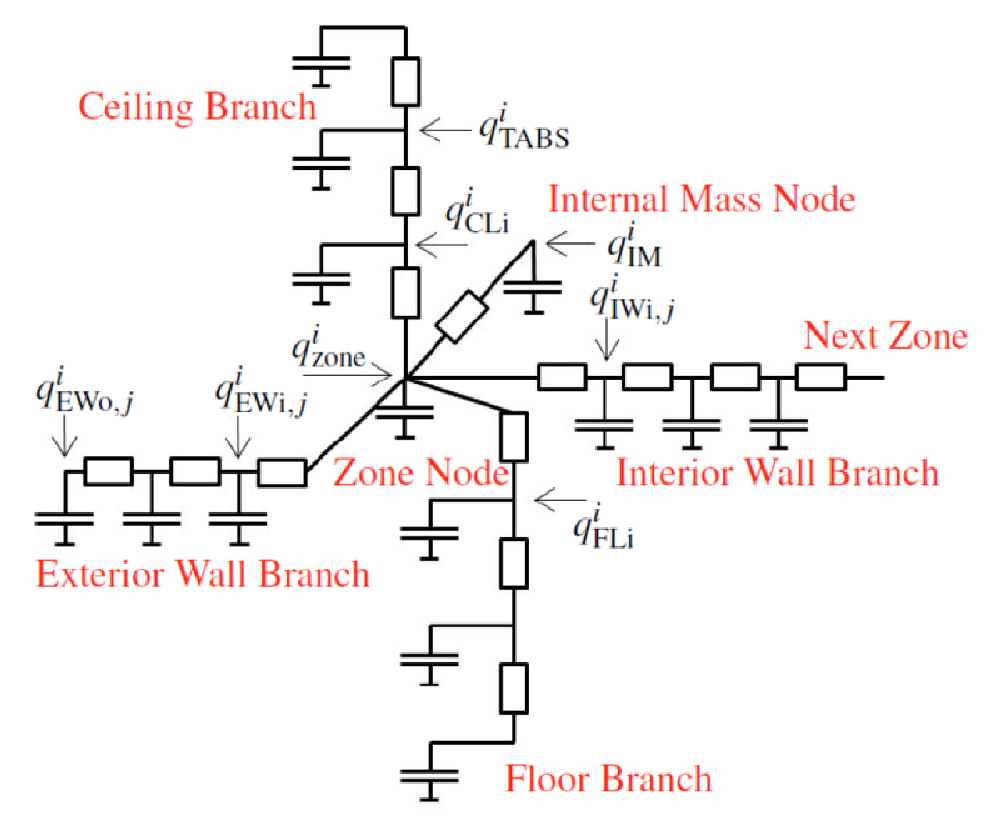
\includegraphics[width=0.6\textwidth]{figures/RC_net.eps}
%				\caption{RC model of a zone. $q$ represents the external heat fluxes}\label{F:RCnet}
%			\end{center}
%		\end{figure}
		The heat exchange between two adjacent layers, i.e. layer "a" and layer "b", was modeled to be proportional to the temperature difference of the two layers and the corresponding thermal resistance $R$, as follows
		\begin{equation}\label{E:RCHeatExchange}
			\begin{aligned}
				&C_a\dot x_a = \left(x_b(t) - x_a(t)\right)/R\\
				&C_b\dot x_b = \left(x_a(t) - x_b(t)\right)/R,
			\end{aligned}
		\end{equation}
		where $C_a$ and $C_b$ are the heat capacitances of the layers. This is done for each layer of each zone, obtaining the compact model \eqref{E:RCZoneEq}. The thermal parameters were derived from zones geometry and materials data.
	\item External heat fluxes were modeled with a bilinear model of the fluxes which are both direct into the building and indirect through elements and zones:
		\begin{equation}\label{E:RCfluxes}
			q(t) = A_q x(t) + B_{q,u}u(t) + B_{q,d}d(t) + \sum_{i=1}^{n_u}{[\left(B_{q,du,i}d(t) + D_{q,xu,i}x(t)\right)u_i(t)]},
		\end{equation}
		with $u$ the inputs and $d$ the disturbances of the system.
		Equation \eqref{E:RCfluxes} comes from a series of 20 equations analyzed in Section 3.3.1.3 of the Technical Report \cite{SturzeneggerTR}, that we do not report here for the sake of simplicity of the treatise. To model the fluxes several information have been considered in the modeling process:
	\begin{itemize}
		\item heat exchange associated with the building hull (except for windows) was modeled considering a conductive and a radiative part;
		\item  heat flux to each Thermally Activated Building System (TABS, i.e. pipes buried in the concrete slabs of the floors carrying hot/cold water) layer was modeled as a fraction of the total supplied TABS heating and cooling heat fluxes;
		\item heat flux through the windows was considered in three different parts: a radiation that directly acts with the elements in contact with the zone's air; a heat flux due to the conduction through the window; a heat flux due to the absorption of the solar radiation from the window;
		\item internal gains due to occupants, appliances and lighting were modeled as a convecting heat acting in each zone;
		\item effects due to the AHU were considered.
	\end{itemize}
	\item The system was discretized.
	\item The resulting model had approximately 300 states for the only second floor, i.e. temperature of the zones, walls and floors. The output of the system were the zone temperatures.
	Since the performance of the state estimation, that is needed to compute the optimal control inputs using MPC, heavily depends on the number of states, an approximated model with fewer states was needed.
	To this aim, different averaged temperatures of the building facades and the zones was considered, obtaining an approximated model with 35 states. The obtained approximated model was then "suitable for use in MPC" (Section 3.3.1.4 of the Technical Report \cite{SturzeneggerTR}). In particular, after the approximation, the resulting model had the following states, inputs and disturbance variables:
	\begin{itemize}
		\item 5 outputs: averaged room temperature for each group of zones (North, South, West, East, Center). The rooms are equipped with temperature sensors.
		\item 18 inputs: TABS heating heat flux; TABS cooling heat flux; averaged transmitted solar heat flux for each group of zones (North, South, West, East), that was estimated using blinds position measurements; air massflow through the energy recovering mode; air massflow bypassing the energy recovering mode; air massflow through the air cooler; AHU heat coil heat flux; lighting power for the offices for each group of zones (North, South, West, East); radiator heat flux in the corner offices (North, South, West, East).
		\item 7 disturbances: internal gains in the offices and internal gains in non-office zones, which were predicted using standard schedule; ambient temperature and solar radiation on facade (North, South, West, East), whose values were obtained through Kalman filtering, using measurements from the weather station placed on the roof of the building. This filtering is needed to take into account the shadowing of the neighboring buildings.
	\end{itemize}
\end{enumerate}
An EnergyPlus model was built for this system, and model parameters of matrices $A_x$, $B_q$, $A_q$, $B_{q,u}$, $B_{q,d}$, $B_{q,du,i}$, $D_{q,xu,i}$ were derived using geometry and materials data from such EnergyPlus model.
This was a choice of the authors, although in a previous work they used real geometry and materials data from the building. 24 parameters needed to be estimated/taken form a datasheet/computed for the considered zone model.
Although some of the parameters are in common between different zones, the others had to be found independently for each zone.
To derive the EnergyPlus model using the available measurements and to use the same control implemented in the building, the EnergyPlus model was coupled with MATLAB using BCVTB software (see \cite{SturzeneggerTR} for more details). To identify the model a total of 294 MATLAB signals were sent to the EnergyPlus model and a total of 1081 EnergyPlus signals were sent back to Matlab.}

\textcolor[rgb]{0,0,1}{This approach suffers of several drawbacks:
\begin{itemize}
	\item in order to keep the model simple, the heat exchange between layers is modeled with a linear behavior as in \eqref{E:RCHeatExchange}. Hence all the nonlinearities are neglected;
	\item in particular cases, as for example the ventilation energy, a linear model is not good enough to provide a good approximation: for this reason a bilinear model was considered.
	However, also in this case, more complex nonlinearities have been neglected due to the already high complexity of the model.
	For example, in \cite{Sturzenegger2016}, the author says "ideally one would want to formulate the optimization problem in terms of set points and operating modes that can be communicated directly to the BAS.
	However, by limiting the model to a bilinear form, this was not possible";
	\item due to the high modeling complexity, different geometries and different materials of the floors have been neglected supposing they are the same for each floor, although this is almost never true in real cases;  
	\item the resulting model was too complex, so it was further approximated to be "suitable for use in MPC" \cite{SturzeneggerTR};
	\item differently from the building geometry, that could be rebuilt by hand, materials data of the building can be unavailable for different reasons (not provided, lost, changed in time).
	Therefore they need to be estimated, hence further increasing the modeling complexity;
	\item due to the high number of states and variables involved in the modeling framework, a lot of measurements are needed to use the model to predict system's behavior.
	This can be cost expensive due to the amount of sensors needed.
	Furthermore, when some measurements are not directly available from the sensors, observers are needed to provide variables estimations.
	However, observability problems could limit the construction of the observers \cite{Dorf2011MCS}. 
\end{itemize}
}

\subsubsection{data-driven modeling example}
\textcolor[rgb]{0,0,1}{Data-driven modeling helps eliminating all the aforementioned problems...}
TO BE DONE $\rightarrow$ \textcolor[rgb]{0,0,1}{Achin}
\begin{itemize}
	\item show procedure
	\item quantify complexity
\end{itemize}


\textcolor[rgb]{0,0,1}{\textbf{Important to add this remark wrt the last bullet point (to answer the reviewer) saying that:} while in the previous case we need to measure all the variables because they are needed to compute model evolution using equations, using machine learning we don't need all the variables (so if we cannot measure everything it is not a problem). This is because the machine learning algorithm creates his internal relation between variables, so also if a variable is missing, the information of the missing variable is present in the behavior of another one. For example: if you don't have the measurement of the energy produced by a photovoltaic panel, the information of the weather conditions will take care of it.}

\textcolor[rgb]{0,0,1}{\textbf{Say also that:} since we don't need to model the state of the walls and floor layers, we don't have that many states as they are, so we don't need to approximate our model and we can consider the temperature of each room as output, without the need of considering an averaged temperature}

\textcolor[rgb]{0,0,1}{\textbf{Advantages:}
\begin{itemize}
	\item we don't need to consider averaged temperatures
	\item we don't need to filter weather data since all the noises are took into account by the machine learning algorithms
	\item we don't need to estimate any parameter
\end{itemize}}

\paragraph{physics-based vs data-driven modeling example}
TO BE DONE $\rightarrow$ \textcolor[rgb]{0,0,1}{Achin}
\begin{itemize}
	\item compare results
\end{itemize}

\paragraph{Objective} The question now is, can we employ data-driven techniques to reduce the cost of modeling and still exploit the benefits that MPC has to offer? Can we build automatic and data-driven approaches for control purposes that are also adaptive, scalable and interpretable? In this paper we address this problem introducing \textit{Data Predictive Control (DPC)} to bridge the gap between Machine Learning and Predictive Control.
\textcolor[rgb]{0,0,1}{
\subsection{Related work}
This section is divided in 3 parts:
\begin{enumerate}
	\item In Section \ref{SSS:ModelBasedWork} we provide a literature review of the approaches that make use of model-based techniques for energy optimization.
	\item In Section \ref{SSS:DataDrivenWork} we report the main works that use of data-driven methodologies for energy optimization and point out the difference with respect to our contribution.
	\item In Section \ref{SSS:PreviousWork} we underline the differences between the results presented in this work and the ones of our previous papers.
\end{enumerate}
\subsubsection{Model-based related work}\label{SSS:ModelBasedWork}
\subsubsection{Data-driven related work}\label{SSS:DataDrivenWork}}
In the literature, several studies deal with the data-driven control techniques using machine learning algorithms \cite{Hou2013}. For example, Artificial Neural Networks are exploited to create data-driven models to be used as plant simulator in closed-loop with a Supervisory Model Predictive Control in \cite{Afram2017}. In \cite{Macarulla2017} the authors proposed a predictive control strategy based on Neural Networks, for boilers control in buildings, to decide the optimal time to switch-on the plan to guarantee energy saving and thermal comfort. However, the strategy is not easily scalable to different types of plants and does not use optimization theory in the closed-loop scheme. In \cite{Costanzo2016} a reinforcement learning control strategy, called Model-Assisted Batch Reinforcement Learning, is considered to provide data-driven control for the demand response problem in HVAC systems. Reinforcement Learning is a model-free methodology and for this reason it can not be used for on-line optimization in a closed-loop predictive control scheme. In \cite{Ferreira2012} the authors considered a data-driven predictive control based on Neural Networks to guarantee energy saving and  thermal comfort in public buildings. Neural Networks are used in the closed-loop control scheme to determine a thermal comfort index based on parameters that can be measured or estimated, but no  system dynamics with internal state are included into the optimization problem. More papers related to this topic can be found in the literature, but to the best of the authors' knowledge none of them address the problem of including data-driven state models in the optimal predictive control loop, and hence allow to set up a MPC-like optimal control problem, as we do in DPC.

\textcolor[rgb]{0,0,1}{
\subsubsection{Previous work}\label{SSS:PreviousWork}
In the following, the differences with respect to our previous papers are illustrated.
\begin{itemize}
	\item In \cite{Behl2016} we	proposed an MPC-like control problem considering regression trees and ensemble methods algorithms for the Demand-Response problem. However, the proposed models allowed to optimally control the system considering only one-step lookahead prediction.
	Hence, it was not possible to use such approach to control the system considering a prediction over an horizon of arbitrary length.
	\item This problem was addressed in \cite{Jain2016}, where the regression trees algorithm was modified to allow the tree to provide multiple-output.
	Each output of the tree was then setup to provide the prediction of the system's behavior over different steps of the predictive horizon.
	This allowed us to setup an MPC-like control problem considering an arbitrary horizon.
	However, in this paper only single regression trees were considered, while ensemble methods were not took into account.
	Modeling accuracy using single trees is strongly subject to the problems of data overfitting and high variance.
	Such approach has the advantage to be extremely simple from the complexity point of view, but its application range is limited to specific kind of systems.
	\item In this work, we extend preliminary results gave in the conference paper \cite{JainCDC2017}.
	An alternative approach is proposed to improve the system's identification accuracy and robustness of the previous approach.
	More precisely, instead of considering a single tree with multiple output, we consider multiple trees with single output.
	Each tree is used to provide the prediction of the system's behavior over different steps of the horizon. With a small increase in complexity, we setup an MPC-like control problem with arbitrary horizon, that provides better results with respect to our previous work. In this paper we further extend this approach to one of the ensemble methods: the random forests.
\end{itemize}
}

\subsection{Main contribution and paper organization}
TO CLARIFY $\rightarrow$ \textcolor[rgb]{0,0,1}{Achin and Francesco}
\begin{itemize}
	\item Add more details
	\item Emphasize difference between Section 4 and Section 5
	\item Cite appendix
\end{itemize}
TO ADD $\rightarrow$ \textcolor[rgb]{1,0,0}{Tullio}
\begin{itemize}
	\item Add references for weather forecast accuracy
	\item Quantify accuracy for short-term prediction for weather forcast to justify the assumption of perfect knowledge for the disturbance
\end{itemize}
TO ADD $\rightarrow$ \textcolor[rgb]{0,0,1}{Achin and Francesco}
\begin{itemize}
	\item Add subsection in Section 5 with simulation of DPC considering disturbance with added noise and show that we still have good performance
\end{itemize}
%In our previous work \cite{Behl2016,Jain2016,JainACC2017,JainCDC2017}, we introduced the concept of DPC for receding horizon control. In this paper, we extend these results providing the following contributions.
%\begin{enumerate}
%	\item In Section \ref{S:dpc}, we formally present the two following control techniques:
%	\begin{enumerate}
%		\item DPC with regression trees, and
%		\item DPC with random forests.
%	\end{enumerate}
%	\item In Section \ref{S:proof}, we demonstrate the strength of DPC for receding horizon control via one-to-one comparison against a benchmark MPC controller using a bilinear building model whose parameters were identified using experiments on a building in Switzerland. We show that DPC captures 70\% variance in MPC and offers a comparable performance.
%	\item Section \ref{S:casestudy} describes a practical application of DPC for Demand Response, where we apply DPC to a 6 story 22 zone building model in EnergyPlus \cite{Crawley2001} for which model-based control is not economical and practical due to extreme complexity. We show scalability and efficiency of DPC in providing financial incentives to the end-customers bypassing the need for high fidelity models. We observe that DPC provides the desired power reduction with an average error of 3\%.
%	\item In Section \ref{S:realCaseStudy}, we implement DPC on the real data from an off-grid house located in L'Aquila (Italy), to find the optimal ON/OFF scheduling for the heating system in order to save energy while guaranteeing thermal comfort for the occupants. We quantify the total amount of energy saved, with respect to the classical bang-bang controller widely used in houses for temperature control, using an EnergyPlus model built specifically for the house. We show we can perform an energy saving that goes from $25.4\%$, if we guarantee thermal comfort, to $49.2\%$, if we allow very little discomfort in terms of rooms' temperature.
%\end{enumerate}

\section{DATA PREDICTIVE CONTROL}
\label{S:dpc}

\textcolor[rgb]{0,0,1}{The central idea behind DPC is to obtain control-oriented models using machine learning methodologies, and formulate the control problem in a way that Receding Horizon Control (RHC) can still be applied and the optimization problem can be solved efficiently. In this paper Regression Trees and Random Forests are considered (see Appendix ??? for details).}

\textcolor[rgb]{0,0,1}{To this aim, let an historical dataset $(\X,\Y)$, created using building measurements, be given to be used in the Regression Trees and Random Forests training process.
Let $|(\X,\Y)| = n$, be the number of samples in the dataset.
$\X = \{(x(k),u(k),d(k))\}$, $\forall k = 1,\ldots,n$, is the set of samples $(x(k),u(k),d(k))$, measured at each time instant $k$, where $x(k)\in\mathbb{R}^{n_x}$ is the vector of the state variables, $u(k)\in\mathbb{R}^{n_u}$ is the vector of the input variables and $d(k)\in\mathbb{R}^{n_d}$ is the vector of the disturbance variables.
$\Y = \{y(k)\},\ \forall k = 1,\ldots,n$, is the set of samples $y(k)$, measured at each time instant $k$, where $y(k)\in\mathbb{R}^{n_y}$ is the vector of the output variables.
We consider $\X$ as the set of predictor variables (or features) and $\Y$ as the set of response variables.
As an example, the response variables can be represented by the power consumption or the room temperatures evolution, while the predictors can be represented by the weather forecast, as the disturbance, the set-points information and building schedules, as the inputs, and room temperatures, as the states. 
Our goal is to learn a data-driven models, using Regression Trees and Random Forests, that relate the value of the response variables with the value of the predictor variables, and that can be used to set up an MPC problem.
}

\textcolor[rgb]{0,0,1}{To do this, we want to derive a model with a closed-form expression of the following form:
\begin{equation}\label{E:GenericModel}
	y(k)=f(x(k),u(k),d(k)),
\end{equation}
where $f$ is an analytical expression that describes the system's dynamics.
\textbf{We want to remark that $y$ can be considered as both a state variable evolution, i.e. $y(k) = x(k+1)$, and a variable that is function of $x$, $u$ and $d$ but is not one of them, as for example is the case of the power. We consider this aspect in Sections \ref{S:proof}, \ref{S:casestudy} and \ref{S:realCaseStudy}. IMPROVE!!!!!!!!!!!!!!!}.
The issue that arises, when using Regression Trees and Random Forests, is that $f$ does not have a closed-form expression, hence \eqref{E:GenericModel} is not suitable for control and optimization.
One possibility could be to look for sub-optimal solutions using evolutionary algorithms \cite{Kusiak2009}, i.e. using heuristics.
In this section we provide a new methodology to determine a closed-form expression for $f$ by manipulating the dataset, as shown starting from Section \ref{SS:sepvar}.}


\subsection{Dataset splitting}
\label{SS:sepvar}

\textcolor[rgb]{0,0,1}{The dataset splitting consists of partitioning the features set $\X$ into the sets $\X^c = \{u(k)\}\subset\X,\ \forall k=1,\ldots,n$, containing the control (or manipulated) variables, and $\X^d = \{(x(k),d(k))\}\subset\X,\ \forall k=1,\ldots,n$, containing the disturbance and state (or non-manipulated) variables.
The union of the two sets forms the full feature set oftraining, i.e. $\X \equiv \X^c \cup \X^d$.
%Our goal is to replace a model-based controller with a data-driven controller, where the latter depends only on the historical sensor data. 
%These measurements could directly represent one or more states in the model-based control framework. We denote these as outputs $\Y \in \R$ for training, i.e. a $\Y$ represents a particular output and we can have separate models for multiple outputs. We define the number of training samples by $|(\X,\Y)| = n$.
Using this splitting methodology, the training process is divided into two steps:
	\begin{enumerate}
		\item the trees and the forests are trained only using $\X^d$, which also eases the computational complexity.
			  It is important to note that besides external disturbance and the state measurements, $\X^d$ can also contains autoregressive terms of the output variables in $\Y$;
		\item in each leaf of the tree (or in each leaf of each the tree of the forest), a linear regression model is trained as a function of the inputs variables in $\X^c$.
		As we shall see in Section~\ref{SS:dpcrt} and \ref{SS:dpcrf}, the second step reduces the run-time control problem into a convex program.
	\end{enumerate}
This process is illustrated in Figure~\ref{F:dpc-sepvars} (left). For the sake of simplicity only trees are considered, but the same holds for the forests. The meaning of the variable $j$ in the linear model in the figure will be clear in the next section.
In Figure~\ref{F:dpc-sepvars} (right), the step 1 of the training process uses also the input variables, i.e. the classical training process without the dataset splitting.
The reason why this latter approach is not suitable for control will be discussed at the end of Section \ref{SS:dpcrt}.
}

\subsection{DPC-RT: DPC with Regression Trees}
\label{SS:dpcrt}
When the data has lots of features, which interact in complicated, nonlinear ways, assembling a single global model such as linear or polynomial regression can be difficult, and can lead to poor response predictions.
\textcolor[rgb]{0,0,1}{As discussed before, an approach to non-linear regression is to partition the data space into smaller regions, where the interactions are more manageable. }
This partition is repeated recursively until we finally get to small chunks of the data space where we can fit simple (eg. linear parametric) models. 
%Therefore, in \eqref{E:sepvars}, the global model $f$ has two parts: the recursive partition $g$, and a linear (and convex) model $h$ for each cell of the partition.

\begin{figure}[t!]
	\centering
	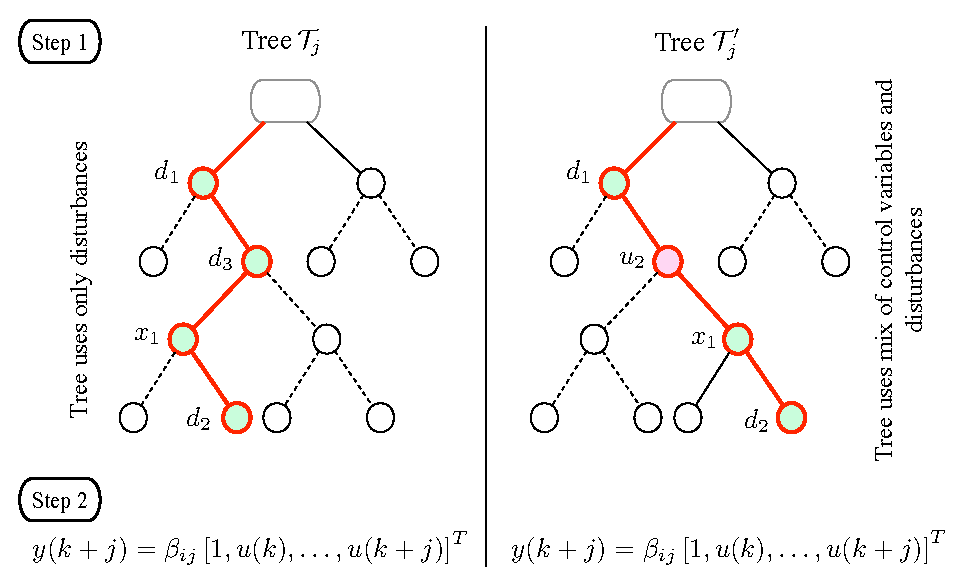
\includegraphics[width=20pc]{figures/dpc-sepvars.eps}
	\caption{Dataset splitting. \textit{Step 1:} Tree $\mathcal{T}_1$ is trained only with variables in $\X^d$ as the features. Tree $\mathcal{T}_2$ uses both the disturbances and states in $\X^d$, and the control variables in $\X_c$ for splitting. It is thus not computationally suitable for control. \textit{Step 2:} In the leaf $\ell_i$ of the trees, a linear regression model parametrized by $\beta_i$ is defined as a function only of the control variables.}
	\captionsetup{justification=centering}
	\label{F:dpc-sepvars}
\end{figure}

\textcolor[rgb]{0,0,1}{Now, in order to have a model that can be used for prediction over an arbitrary long horizon in an MPC problem, our goal is to predict, at time $k$, the output $y$ for next $N$ time steps, i.e. $y(k),\ldots,y(k+N)$, where $N$ is the control horizon, given the state measurements, i.e. $x(k)$, and the disturbance forecast, i.e. $\tilde d(k),\ldots,\tilde d(k+N)$, at time $k$.
For the sake of simplicity and without any loss of generality, in the following, we consider only a single output, i.e. $y(k)\in\mathbb{R}$ (or $n_y = 1$).
However, as we will see in Sections \ref{S:casestudy} and \ref{S:realCaseStudy}, multiple trees (or forests) can be built for multiple outputs.
Applying the dataset splitting, we build $N$ regression trees using CART procedure \cite{Breiman1984} (see also Appendix for more details), such that the output $y(k+j)$ of the $j^{th}$ tree depends upon the previous $\delta_d$ disturbances, and on the state at instant $k$ and its $\delta_x$ regressive terms:
\begin{equation}\label{E:model_tree}
\T_j = \mathit{f}_{\mathrm{tree}} \left( d(k+j-\delta_d),\ldots,d(k+j),x(k-\delta_x),\ldots,x(k)  \right),\ j=1,\ldots,N,
\end{equation}
with $\left( d(k+j-\delta_d),\ldots,d(k+j),x(k-\delta_x),\ldots,x(k)  \right)\in\X^d,\ k=1,\ldots,n$, and $\mathit{f}_{\mathrm{tree}}$ representing the tree structure.
Then, the linear models, as functions of the inputs variables $u\in\X^c$, in each leaf of the trees $\T_j,\ j=1,\ldots,N$, are defined as
\begin{equation}\label{E:model_leaf}
y(k+j) =  \beta_j [1,u(k),\ldots,u(k+j) ]^T,\ j=1,\ldots,N.
\end{equation}}
Note that the coefficients $\beta_j$ are different for each leaf.
Equation~\eqref{E:model_leaf} implies that the prediction of output $y(k+j)$ at time $k$ is an affine combination of control inputs from time $k$ to $k+j$.
Thus, we have managed to linearize the original model dynamics via black-box modeling.
\textcolor[rgb]{0,0,1}{One of the advantages of this approach is that this two-step training is done off-line, so the time required to create the models does not affect the control execution in run-time.}

\textcolor[rgb]{0,0,1}{The problem now is: \emph{how to use this modeling framework to set up an MPC problem?} In run-time, given the disturbance forecast and the state measurements at time $k$, i.e. $\tilde d(k+j-\delta_d),\ldots,\tilde d(k+j),x(k-\delta_x),\ldots,x(k)$ given $k$, we can narrow down to a leaf of each tree in \eqref{E:model_tree} to retrieve the linear models in \eqref{E:model_leaf} for each step $j=1,\ldots,N$ of the horizon (see first part of the pseudo code given in Algorithm \ref{A:dpcrt}), as depicted in Figure \ref{F:dpc-sepvars} (left). These models are used to setup the MPC Problem \ref{P:dpcrt}.
In particular, }when a new control action has to be determined, each tree (prediction step) contributes to a linear constraint in the optimization as a replacement for the state dynamics in the case of MPC. Thus, the MPC optimization problem, considering a quadratic cost ($Q \succeq 0, R \succeq 0$) function and the general case of multiple outputs, i.e. $y(k)\in\mathbb{R}^{n_y},\ n_y\geq 1$, can be formulated as:
%\begin{problem}\label{P:dpcrt}
%	\begin{equation}
%		\begin{aligned}
%		\text{min } & \sum_{j=1}^{N} ({\Y}_{\mathrm{k+j|k}})^2 \mathcal{Q} + {\X^c}^T_{\mathrm{k+j-1|k}} \mathcal{R} {\X^c}_{\mathrm{k+j-1|k}} + \lambda\epsilon_j\\
%		\text{s.~t. } & \ \ \ \ \ \Y_{\mathrm{k+j|k}} =  \beta^T [1,\X^c_{\mathrm{k|k}},\dots,\X^c_{\mathrm{k+j-1|k}} ]^T \\
%		& \ \ \ \ \ \ \ \ \ \ \ \ \ \ \ \underline{\X}^c \leq \X^c_{\mathrm{k+j-1|k}} \leq \bar{\X}^c\\ 
%		& \ \ \ \ \ \ \ \ \ \ \ \ \underline{\Y}-\epsilon_j \leq \Y_{\mathrm{k+j|k}} \leq \bar{\Y} + \epsilon_j\\\
%		& \ \ \ \ \ \ \ \ \ \ \ \ \ \ \epsilon_j \geq 0, \ j = 1,\dots,N.
%		\end{aligned}
%		\label{E:dpcrt}
%	\end{equation}
%\end{problem}
\begin{problem}\label{P:dpcrt}
	\begin{equation}
	\begin{aligned}
	& \underset{u_{k+j}}{\text{minimize}} & & \sum_{j=1}^{N} y^\top_{k+j} Q y_{k+j} + u^\top_{k+j} R u_{k+j} + \lambda\epsilon_j \\
	& \text{subject to }                  & & y_{k+j}     =   \beta_j [1,u_{k},\ldots,u_{k+j} ]^\top                             \\
	&                                     & & u_{k+j}    \in  \mathcal{U}                                                        \\
	&                                     & & |y_{k+j}|  \leq \bar{y}_{k+j} + \epsilon_j 										 \\
	&                                     & & \epsilon_j \geq  0							                                     \\
	&                                     & & j           =    1,\ldots,N.            									         \\
	\end{aligned}
	\label{E:dpcrt}
	\end{equation}
\end{problem}

\textcolor[rgb]{0,0,1}{Here, $Q \in \mathbb{R}^{n_y\times n_y}$ and $R \in \mathbb{R}^{n_u\times n_u}$ are weight matrices used to give more importance in the minimization to either $y$ or $u$.
This problem is solved as in the classical MPC formulation, i.e. at each time step $k=1,2,\ldots$ the optimal control sequence $u^*_k,\ldots,u^*_{k+N}$ is computed, and only the first input of the sequence is applied as control input to the system: $u(k) = u^*_k$.
The slack variables $\epsilon_j$ are added to ensure recursive feasibility (since the equality constraint on $y$ is relaxed), i.e. to guarantee that Problem \ref{P:dpcrt} can provide a solution at each step $k=1,2,\ldots$.
$\lambda$ is a weight used to give more importance to bounds violation with respect to $y$, than to the cost function optimization, and viceversa. 
Of course, a different cost function can be chosen depending upon the application, i.e. it can be linear, nonlinear, etc., obviously changing the complexity of the problem.
In the current formulation, the data-driven control problem is reduced to a convex program which is very easy and efficient to solve.}
The pseudo code for DPC-RT is given in Algorithm~\ref{A:dpcrt}.
\textcolor[rgb]{0,0,1}{DPC algorithm is also graphically shown in Figure \ref{F:dpc-algo-rf} for the random forest case, but the same holds for single regression trees.}

\textcolor[rgb]{0,0,1}{\begin{remark}
	 If we did not consider the splitting procedure	of the dataset, and we also used input variables to learn the trees, as in the right side of Figure 1, the resulting
	 model would not have been suitable for control. This is because, since u is the variable we want to optimize, we do not know its value a priori to go through the trees and determine the correct leaves to find the models to use in the RHC problem.
\end{remark}}

\begin{algorithm}[t!]
	\caption{Data Predictive Control with Regression Trees}
	\label{A:dpcrt}
	\begin{algorithmic}[1]
		\State \textsc{Design Time (Off-Line)}
		\Procedure{Model Training using Dataset Splitting}{}
		\State Set $\X^c$ $\gets$ manipulated features
		\State Set $\X^d$ $\gets$ non-manipulated features
		\State Build $N$ predictive trees with $(\X^d,\Y)$ as defined in \eqref{E:model_tree}
		\ForAll{trees $\mathcal{T}_j$}
		\ForAll{the leaves $\ell_i$ of $\mathcal{T}_j$}
		\State Fit $ y(k+j) =  \beta_j \left[1,u(k),\ldots,u(k+j) \right]^T$ as in \eqref{E:model_leaf}
		\EndFor
		\EndFor
		\EndProcedure
		\State \textsc{Run Time}
		\Procedure{Predictive Control}{}
		\While{$k< k_{\mathrm{stop}}$}
		\ForAll{trees $\mathcal{T}_j$}
		\State Determine the leaf $\ell_i$ using $\X^d$ as in \eqref{E:model_tree}
		\State Obtain the linear model at $\ell_i$ trained in \eqref{E:model_leaf}
		\EndFor
		\State Solve optimization problem \ref{P:dpcrt} to determine optimal
		\State control actions $u^*_k,\ldots,u^*_{k+j}$
		\State Apply the first input $u(k)=u^*_k$
		\EndWhile
		\EndProcedure
	\end{algorithmic}
\end{algorithm}

\subsection{DPC-En: DPC with Ensemble Methods}
\label{SS:dpcrf}
Regression trees obtain good predictive accuracy in many domains. However, the models used in their leaves have some limitations regarding the kind of functions they are able to approximate.
The problem with trees is their high variance and that they can overfit the data easily.
A small change $\delta$ in the data can result in a different series of splits and thus violate the acceptable accuracy.
This is the price to be paid for estimating a tree-based structure from the data.


We use ensemble methods \cite{Friedman2001}, in particular Random Forests, to combine the predictions of several independent regression trees in order to improve generalizability and robustness over a single estimator. 
The essential idea is to average many noisy trees to reduce the overall variance in prediction.
We inject randomness into the tree construction in two ways. First, we randomize the features used to define splitting in each tree.
Second, we build each tree using a bootstrapped or sub-sampled data set.
In this way, each tree in the forest is trained on different data, which introduces differences between the trees.
\textcolor[rgb]{0,0,1}{More explicitly, training features $\bar{\X}^d_i\subset\X^d$, $i=1,2,...$ and the in-bag samples (in-bag samples correspond to the data samples which each tree was trained on) are different for each tree in the forest, i.e $|(\bar \X^d_i,\bar\Y_i)|<n$, with $\bar\Y_i\subset\Y$.}

\textcolor[rgb]{0,0,1}{The goal with DPC-En is to replace each tree in Algorithm~\ref{A:dpcrt} by a forest.
This can be done replacing Equations \eqref{E:model_tree} and \eqref{E:model_leaf} with the Equations \eqref{E:model_forest} and \eqref{E:model_leaf_forest} provided in the following:
\begin{equation}\label{E:model_forest}
\F_j = \mathit{f}_{\mathrm{forest}} \left( d(k+j-\delta_d),\ldots,d(k+j),x(k-\delta_x),\ldots,x(k)  \right),\ j=1,\ldots,N,
\end{equation}
with $\left( d(k+j-\delta_d),\ldots,d(k+j),x(k-\delta_x),\ldots,x(k)  \right)\in\X^d,\ k=1,\ldots,n$, and $\mathit{f}_{\mathrm{forest}}$ representing the forest structure.
In particular, as mentioned above, each tree $\T_i$ of each forest $\F_j$ is trained using $(\bar \X^d_i,\bar\Y_i)$.
Then the linear models, as functions of the inputs variables $u\in\bar\X^c_i\subset\X_c$, in each leaf of each tree of the forests $\F_j,\ j=1,\ldots,N$, are defined as
\begin{equation}\label{E:model_leaf_forest}
y(k+j) =  \Theta_{ij} [1,u(k),\ldots,u(k+j) ]^T,\ j=1,\ldots,N.
\end{equation}
Here $(\bar\X^c_i,\bar\Y_i)$ correspond to the in-bag samples for the trees.}

While the off-line training burden in DPC-En is slightly increased compared to DPC-RT, in the control step we exploit the better accuracy, and lower variance properties of the random forests. 
If a forest has $t$ number of trees, given the forecast of disturbances, we have $t$ sets of linear coefficients. We simply average out all the coefficients from all the trees to get one linear model represented by $\hat{\Theta}_j$ for each forest. Note that the averaging step can only be done in run-time, because the leaf of each tree can be narrowed down only when the $\X^d$ is known. Thus, for $N$ forests, we again have exactly $N$ linear equality constraints as in the optimization problem below:

\begin{problem}\label{P:dpcrf}
	\begin{equation}
	\begin{aligned}
	& \underset{u_{k+j}}{\text{minimize}} & & \sum_{j=1}^{N} y^\top_{k+j} Q y_{k+j} + u^\top_{k+j} R u_{k+j} + \lambda\epsilon_j \\
	& \text{subject to }                  & & y_{k+j}      =  \hat{\Theta}_j [1,u_{k},\ldots,u_{k+j} ]^\top                      \\
	&                                     & & u_{k+j}    \in  \mathcal{U}                                                        \\
	&                                     & & |y_{k+j}|  \leq \bar{y}_{k+j} + \epsilon_j 										 \\
	&                                     & & \epsilon_j \geq  0							                                     \\
	&                                     & & j           =    1,\ldots,N.            									         \\
	\end{aligned}
	\label{E:dpcrf}
	\end{equation}
\end{problem}
DPC-En is graphically described in Figure~\ref{F:dpc-algo-rf}.

The ensemble data predictive control (DPC-En) is the first such method to bridge the gap between ensemble predictive models (such as random forests) and receding horizon control. In the next section, we compare DPC-RT and DPC-En to MPC for a building model.

\begin{figure}[t!]
	\centering
	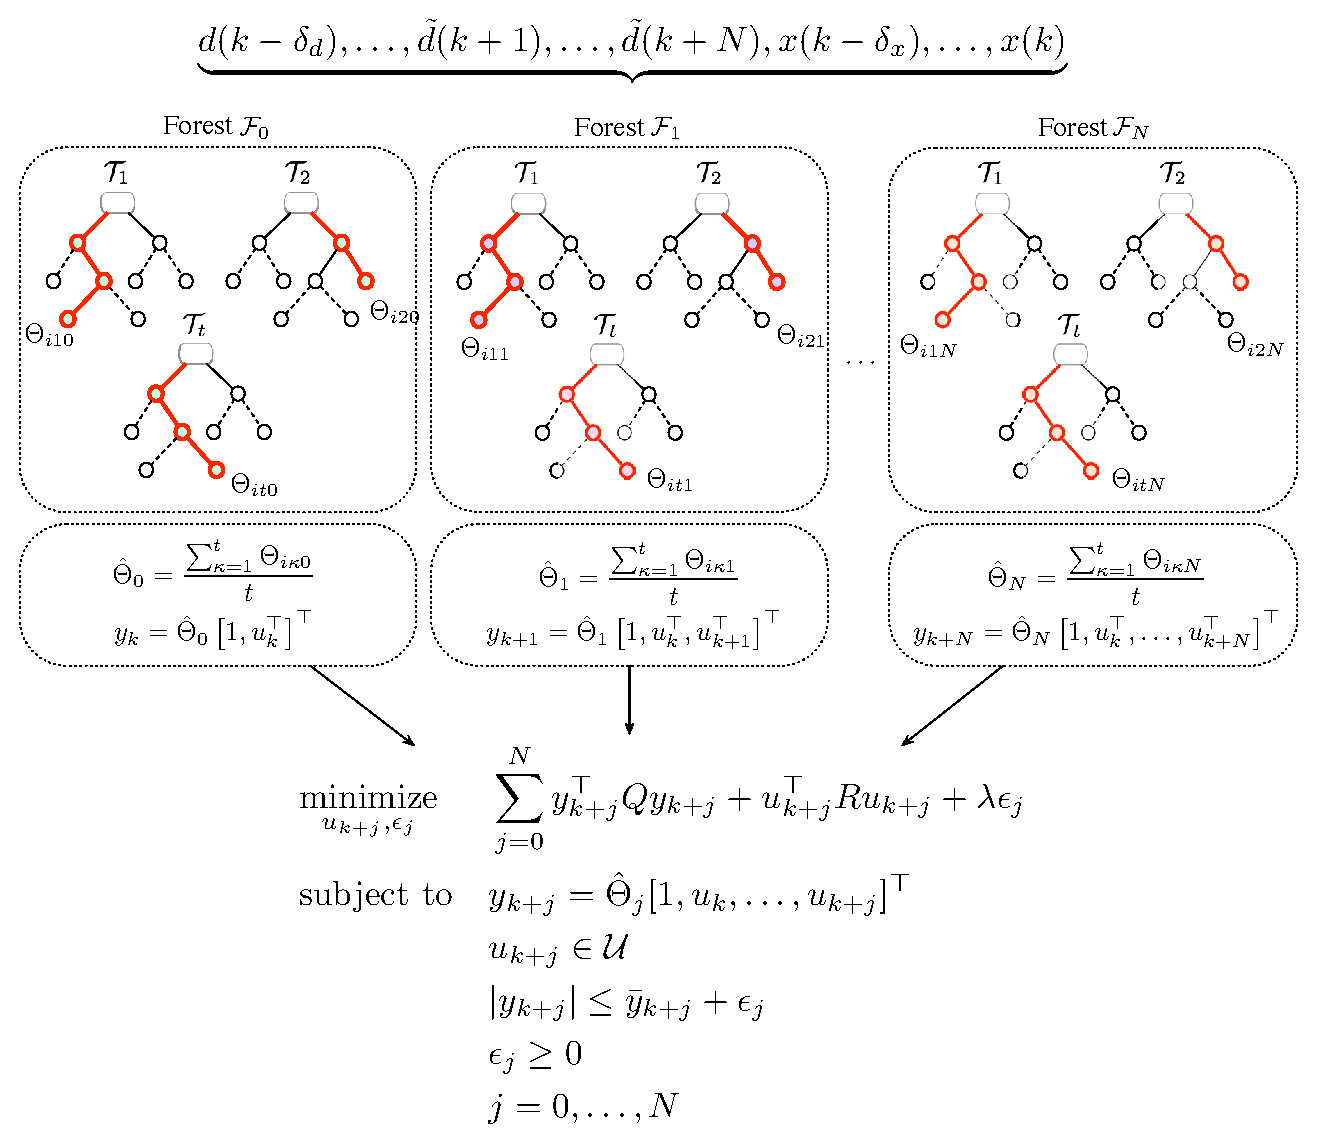
\includegraphics[width=26pc]{figures/dpc-algo-rf.eps}
	\caption{\textcolor[rgb]{0,0,1}{DPC-En: At time $k$, the algorithm uses the forecast of disturbances and the state measurements in $\X^d$ at time $k$ to select linear models $\Theta_1$ to $\Theta_t$ in the leaves of each forest. The linear models in each forest are averaged to calculate a single model represented by $\hat{\Theta}_j$, and act as constraints in the optimization problem. The optimal sequence $u^*_k,\ldots,u^*_{k+N}$, of which only the first element is applied, i.e. $u(k)=u^*_k$, and variables in $\X^d$ at time $k+1$ are calculated to proceed to next step at $k+1$.}}
	\label{F:dpc-algo-rf}
\end{figure}

\section{COMPARISON WITH MPC}
\label{S:proof}

We consider a bilinear building model developed at Automatic Control Laboratory, ETH Zurich.
It captures the essential dynamics governing the zone-level operation while considering the external and the internal thermal disturbances. 
By Swiss standards, the model used for this study is of a heavyweight construction with a high window area fraction on one facade and high internal gains due to occupancy and equipments \cite{Gyalistras2010a}. 

The bilinear model is a standard building model used for practical considerations \cite{Ma2015,Oldewurtel2011,Oldewurtel2012} as it is detailed enough and suitable for model-based control unlike the ones obtained from simulation software like EnergyPlus. We specifically consider this model to show a comparison against MPC. 
MPC of EnergyPlus models can be cost and time prohibitive, making them unsuitable for control. In Sec.~\ref{S:casestudy}, we show how DPC scales easily to such large scale models.

\subsection{Bilinear Model}
\label{SS:model}
%The building is treated as a lumped-parameter system, which assumes nodes in the room as well as in the walls, floor, and ceiling describing the respective temperatures.
%Considering the heat transfer rate between the nodes, an equivalent thermal RC network is identified. 
%The influence of the actuators is modeled according to their heat transfer properties, e.g. the heating input from the radiator goes directly into the room node, whereas floor heating affects the room with some delay and therefore the control input from floor heating goes into the node in the floor.

The bilinear model has 12 internal states including the inside zone temperature $\mathsf{T}_{\mathrm{in}}$, the slab temperatures $\mathsf{T}_{\mathrm{sb}}$, the inner wall $\mathsf{T}_{\mathrm{iw}}$ and the outside wall temperature $\mathsf{T}_{\mathrm{ow}}$. The state vector is defined as $x:=[\mathsf{T}_{\mathrm{in}}, \mathsf{T}_{\mathrm{sb}}^{(1:5)}, \mathsf{T}_{\mathrm{ef}}^{(1:3)}, \mathsf{T}_{\mathrm{in}}^{(1:3)}]^T$.

There are 4 control inputs including the blind position $\mathsf{B}$, the gains due to electric lighting $\mathsf{L}$, the evaporative cooling usage factor $\mathsf{C}$, and the heat from the radiator $\mathsf{H}$ such that $u:=[\mathsf{B},\mathsf{L},\mathsf{H},\mathsf{C}]^T$. $\mathsf{B}$ and $\mathsf{L}$ affect both room illuminance and temperature due to heat transfer whereas $\mathsf{C}$ and $\mathsf{H}$ affect only temperature.

The model is subject to 5 weather disturbances: solar gains with fully closed blinds $\mathsf{Q}_{\mathrm{sc}}$ and with open blinds $\mathsf{Q}_{\mathrm{so}}$, daylight illuminance with open blinds $\mathsf{I}_{\mathrm{o}}$, external dry-bulb temperature $\mathsf{T}_{\mathrm{db}}$ and external wet-bulb temperature $\mathsf{T}_{\mathrm{wb}}$. 
The hourly weather forecast, provided by MeteoSwiss, was updated every 12 hrs. Therefore, to improve the forecast,  an autoregressive model of the uncertainty was considered.
Other disturbances come from the internal gains due to occupancy $\mathsf{Q}_{\mathrm{io}}$ and due to equipments $\mathsf{Q}_{\mathrm{ie}}$ which were assumed as per the Swiss standards \cite{Merkblatt2006}. We define $d:=[\mathsf{Q}_{\mathrm{sc}},\mathsf{Q}_{\mathrm{so}},\mathsf{I}_{\mathrm{o}},\mathsf{Q}_{\mathrm{io}},\mathsf{Q}_{\mathrm{ie}},\mathsf{T}_{\mathrm{db}},\mathsf{T}_{\mathrm{wb}}]^T$. For further details, we refer the reader to \cite{Oldewurtel2011}.

The model dynamics is given below. The bilinearity is present in both input-state, and input-disturbance.
\begin{gather}
\label{E:bilinear1}
x_{k+1} = Ax_{k}+(B_u +B_{xu}[x_k] + B_{du}[d_k]) u_k+B_dd_k \\
x_{k} \in \mathbb{R}^{12}, u_{k} \in \mathbb{R}^{4}, d_{k} \in \mathbb{R}^{8} \ \forall k = 0,\dots,T, \nonumber
\end{gather}
where, the matrices $B_{xu}$ and $B_{du}$ are defined as
\begin{gather}
\label{E:bilinear2}
B_{xu}[x_k] = [ B_{xu,1}[x_k],B_{xu,2}[x_k], \dots, B_{xu,4}[x_k] ] \in \mathbb{R}^{12\times4}, \nonumber\\
B_{du}[d_k] = [ B_{du,1}[d_k],B_{du,2}[d_k], \dots, B_{du,4}[d_k] ] \in \mathbb{R}^{12\times4}\nonumber, \\
B_{xu,i} \in \R^{12\times12}, B_{du,i} \in \R^{12\times8} \ \forall i=1,2,3,4.\nonumber
\end{gather}
For this study, we assume that the disturbances are precisely known to MPC as well as DPC controller. In our future work, we will account for the uncertainties in the disturbances with an extension to Scenario approach \cite{Bernardini2009} for DPC.

\begin{figure}[t!]
	\centering
	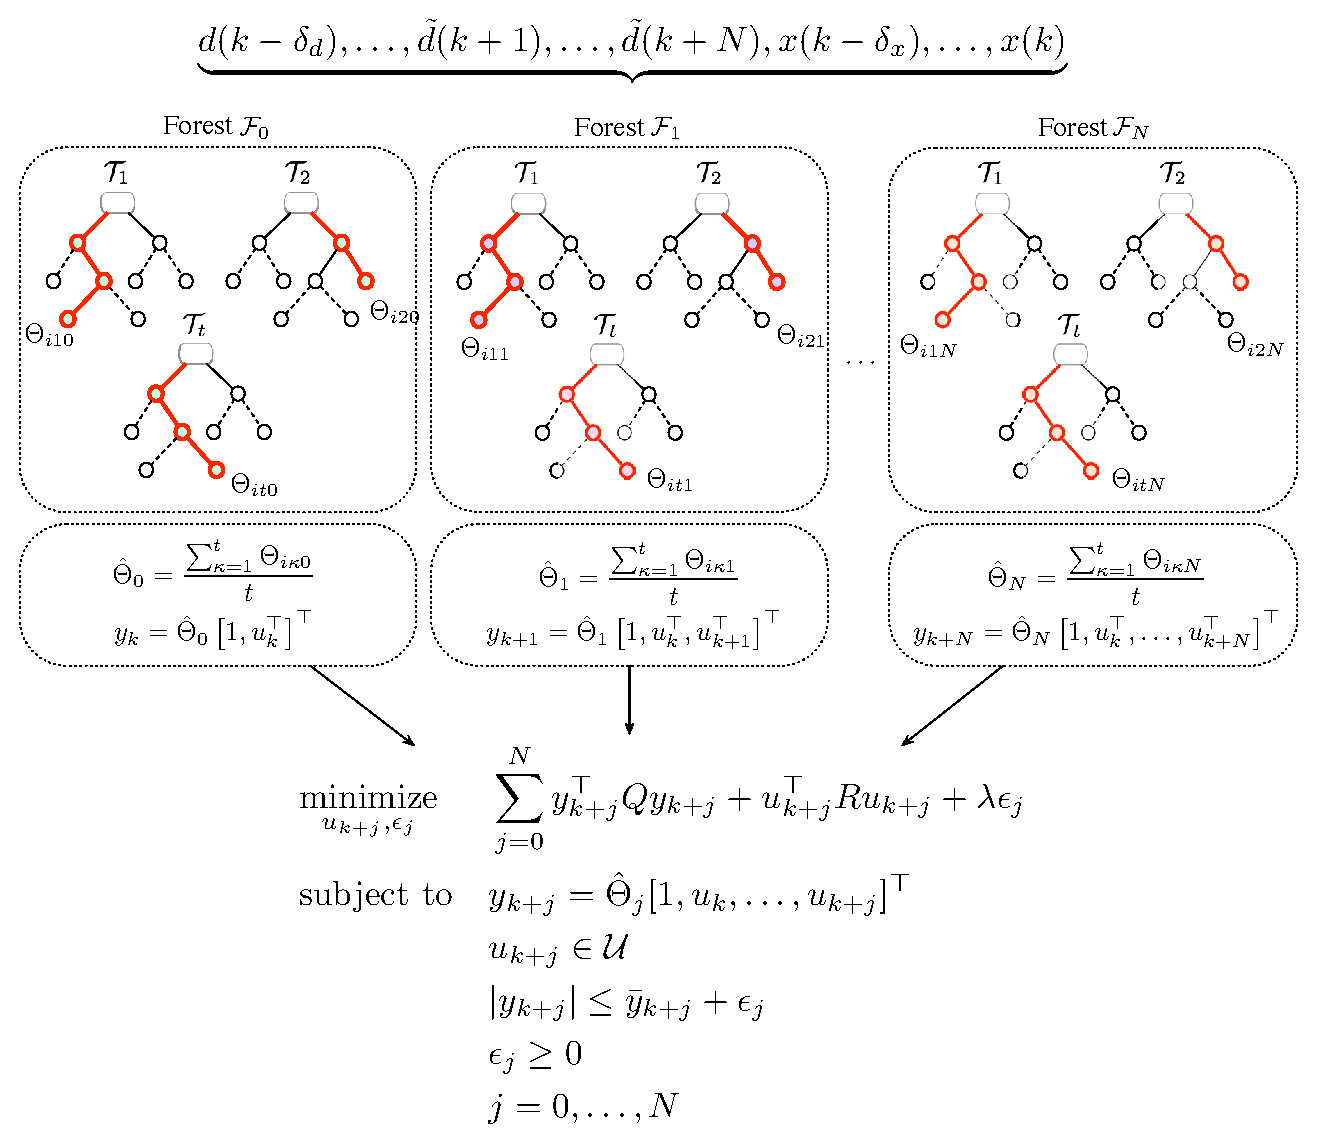
\includegraphics[width=21pc]{figures/dpc-algo-rf.eps}
	\caption{DPC-En: At time $k$, the algorithm uses the forecast of disturbances $\tX^d_{\mathrm{k|k}}$ to select linear models $\Theta_1$ to $\Theta_t$ in the leaves of each ensemble. The linear models in each ensemble are averaged to calculate a single model represented by $\hat{\Theta}_j$ which act as constraints in the optimization problem. The optimal sequence $[\tX^c_{\mathrm{k|k}},\dots,\tX^c_{\mathrm{k+N-1|k}}]$, of which the first one is applied, and $\tX^d_{\mathrm{k+1|k+1}}$ is calculated to proceed to $k+1$.}
	\label{F:dpc-algo-rf}
\end{figure}

\subsection{Model Predictive Control}
\label{SS:mpc}
We use an MPC controller with a quadratic and a linear cost for comparison.
The finite RHC approach involves optimizing a cost function subject to the dynamics of the system and the constraints, over a finite horizon of time \cite{Mayne2000}. After an optimal sequence of control inputs are computed, the first input is applied, then at the next step the optimization is solved again.

%\begin{figure}
%\centering
%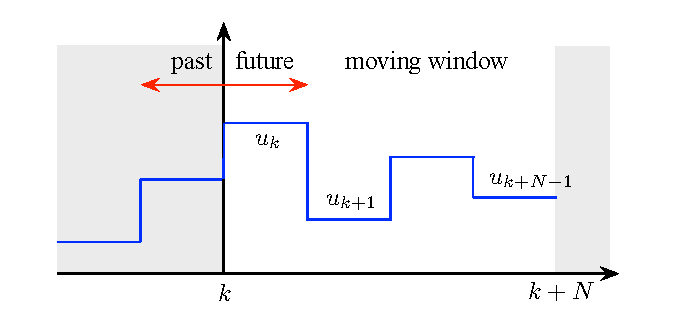
\includegraphics[scale=0.8]{figures/mpc_horizon.eps}
%\caption{Finite-horizon moving window of MPC: at time $k$, the MPC optimization problem is solved for a finite length window of $N$ steps and the first control input $u_k$ is applied; the window then recedes one step forward and the process is repeated at time $k+1$.}
%\captionsetup{justification=centering}
%\label{F:mpc}
%\end{figure}

The objective of the controller is to minimize the energy usage $c^Tu$ while maintaining a desired level of thermal comfort.
Therefore, at time step $k$, we solve a continuously linearized MPC problem to determine the optimal sequence of inputs $[u_{\mathrm{k|k}},\dots,u_{\mathrm{k+N-1|k}}]$:
\begin{subequations}
\begin{align}
\text{min } & \ \ \ \ \sum_{j=1}^{N} {x}^T_{\mathrm{k+j|k}} \mathcal{Q} {x}_{\mathrm{k+j|k}} + c^Tu_{\mathrm{k+j-1}} +  \lambda\epsilon_j\\
\text{s.~t. } & \ \ x_{\mathrm{k+j|k}} =  Ax_{\mathrm{k|k}} + B u_{\mathrm{k+j-1|k}} + B_d d_{\mathrm{k+j-1|k}} \label{SE:mpc1} \\
& \ \ \ \ \ B = B_u + B_{xu}[x_{\mathrm{k|k}}] + B_{du}[d_{\mathrm{k+j-1|k}}] \label{SE:mpc2}\\
& \ \ \ \ \ \ \ \ \ \ \ \ \ \ \ \underline{u} \leq u_{\mathrm{k+j-1|k}} \leq \bar{u}\\ 
& \ \ \ \ \ \ \ \ \ \ \ \ \underline{x}-\epsilon_j \leq x_{\mathrm{k+j|k}} \leq \bar{x} + \epsilon_j\\\
& \ \ \ \ \ \ \ \ \ \ \ \ \ \ \epsilon_j \geq 0, \ j = 1,\dots,N,
\end{align}\label{E:mpc}
\end{subequations} 
\noindent where $\mathcal{Q} \in \R^{12 \times 12}$ has all zeros except at $\mathcal{Q}^{(1,1)}$ corresponding to the zone temperature, $c \in \R^{4}$ is proportional to cost of using each actuator and $\lambda$ penalizes the slack variables.

\subsection{Data Predictive Control}
\label{SS:dpc}
In this section, we explain how DPC can be applied to this case study. We begin with a description of features $\tX$ and output $\tY$ used for training.

\subsubsection{Training Data} 
\label{SSS:dpc_data}

The fundamental reason why DPC  is suitable for such a problem is that when the complexity rises, there is a huge cost to model all the states given by the dynamical system \eqref{E:bilinear1}. For example, states in the bilinear model also include slab temperatures which require modeling of structural and material properties in detail and often we also need to install new sensors to capture additional states. Thus, DPC is based solely on one state of the model i.e. the zone temperature that can be easily measured with a thermostat. This serves as the output variable $\tY$ of interest for which we build $N$ trees and $N$ forests as described in Sec.~\ref{SS:dpcrt} and \ref{SS:dpcrf}, respectively. Therefore, $\tY_{\mathrm{k+j|k}}:=x_{\mathrm{k+j|k}}^1$, where $x^1$ is the first component of $x$.
Next, we define the non-manipulated features $\tX^d_{\mathrm{k|k}}$. At time $k$, for the tree $\mathcal{T}_j$ and the forest $\mathcal{R}_j$, we base these features to include weather disturbances, external disturbances due to occupancy and equipments, and autoregressive terms of the room temperature, i.e.
$\tX^d_{\mathrm{k|k}}:=[ d_{\mathrm{k+j-N|k}} ,\dots,d_{\mathrm{k+j-1|k}}, x_{\mathrm{k|k}}^1,\dots, x_{\mathrm{k-\delta|k}}^1 ]$, where $\delta$ is the order of autoregression.
Finally, the inputs in DPC are exactly same as in MPC. i.e. $\tX^c_{\mathrm{k+j-1|k}}:=u_{\mathrm{k+j-1|k}}$.

The training data in the above format was generated by simulating the bilinear model with rule-based strategies for 10 months in 2007. January and May were deliberately excluded for testing the DPC implementation.

\subsubsection{Optimization} 
\label{SSS:dpc_opt}
For a fair comparison with MPC, we cast DPC optimization problem as follows:
\begin{subequations}
\begin{align}
\text{min } & \sum_{j=1}^{N} {\tY}_{\mathrm{k+j|k}} \mathcal{Q}^{(1,1)} {\tY}_{\mathrm{k+j|k}} + c^T \tX^c_{\mathrm{k+j-1|k}}+  \lambda\epsilon_j\\
\text{s.~t. } & \ \ \ \ \ \tY_{\mathrm{k+j|k}} =  \alpha_j^T \left[1,\tX^c_{\mathrm{k|k}},\dots,\tX^c_{\mathrm{k+j-1|k}} \right]^T \label{SE:dpc}\\
& \ \ \ \ \ \ \ \ \ \ \ \ \ \ \ \underline{\tX}^c \leq \tX^c_{\mathrm{k+j-1|k}} \leq \bar{\tX}^c\\ 
& \ \ \ \ \ \ \ \ \ \ \ \ \underline{\tY}-\epsilon_j \leq \tY_{\mathrm{k+j|k}} \leq \bar{\tY} + \epsilon_j\\\
& \ \ \ \ \ \ \ \ \ \ \ \ \ \ \epsilon_j \geq 0, \ j = 1,\dots,N.
\end{align} \label{E:dpc}
\end{subequations}
\noindent Here $\alpha = \beta$ for DPC-RT and $\alpha = \hat{\Theta}$ for DPC-En.
Note that, \eqref{E:dpc} is DPC analog of \eqref{E:mpc}. The only difference is the state dynamics \eqref{SE:mpc1} and \eqref{SE:mpc2} are now replaced with \eqref{SE:dpc}.

\subsubsection{Validation} 
\label{SSS:dpc_val}

We compare the prediction for the first time step $\tY_{\mathrm{k+1|k}}$ and the 6-hour ahead prediction $\tY_{\mathrm{k+6|k}}$ for a week in the month of May in Fig.~\ref{F:validation}. It is visible how trees have a high variance, and the forests are more accurate. Note that data from January and May was not used for training. The quantitative summary of the accuracy is given in Tab.~\ref{T:validation}. We can see that the random forests are better in all respects.
\begin{table}[h!]
	\centering
	\caption{Quantitative comparison of root mean square error (RMSE), $R^2$ score, and explained variance (EV) for trees and forests for different predictions steps.}
	\captionsetup{justification=centering}
	\begin{tabular}{c|c|c|c}
		\toprule
		& RMSE & $R^2$ score & EV  \\ 
		\midrule
		tree-$\tY_{\mathrm{k+1|k}}$    &  0.42 &  0.75 & 0.76    \\
		tree-$\tY_{\mathrm{k+6|k}}$  & 0.64 &  0.41  & 0.42 \\
		forest-$\tY_{\mathrm{k+1|k}}$  & 0.29 & 0.87  & 0.88 \\
		forest-$\tY_{\mathrm{k+6|k}}$  & 0.38 & 0.78 & 0.80 \\
		\bottomrule
	\end{tabular}
	\label{T:validation}
\end{table}

\begin{figure}[h!]
	\centering
	\includegraphics[width=20pc]{figures/validation-s1.eps}
	\includegraphics[width=20pc]{figures/validation-s6.eps}
	\caption{Temperature predictions from a tree and a forest for first step prediction (top) and the 6-hour ahead prediction (bottom). Ensemble method shows a relatively higher accuracy.}
	\captionsetup{justification=centering}
	\label{F:validation}
\end{figure}

%\begin{figure}[t!]
%	\centering
%	\includegraphics[width=20pc]{figures/validation-s6.eps}
%	\caption{Temperature predictions from a tree and a forest for 6 hour ahead prediction.}
%	\captionsetup{justification=centering}
%	\label{F:validation-s6}
%\end{figure}

\subsection{Comparison}
\label{SS:comp}
We compare the performance of DPC \eqref{E:dpc} against an equivalent MPC formulation \eqref{E:mpc}. The solution obtained from MPC sets the benchmark that we compare to. Note that the MPC implementation uses the exact knowledge of the plant dynamics. Therefore, the associated control strategy is indeed the optimal strategy for the plant.

The performance is compared for 3 days in winter, i.e. January 28-31 and 3 days in summer, i.e. May 1-3. These are shown on the same plots in Figure~\ref{F:comparison}.
The sampling time in the simulations is 1 hr. The control horizon $N$ and the order of autoregression are both 6 hrs. The training procedure required a few minutes in the case of trees and 2 hrs for forests on a Win 10 machine with an i7 processor and 8GB memory.
The cooling usage factor $\mathsf{C}$ is constrained in $[0,1]$, the heat input in $[0,23]\ \mathrm{W/m^2}$, and the room temperature in $[19,25]\ \mathrm{^oC}$ during the winters and $[20,26]\ \mathrm{^oC}$ during the summers.
The optimization is solved using CPLEX \cite{IBM}.

The external disturbances - solar gain, internal gain due to equipment and dry-bulb temperature during the chosen periods are shown in Figure~\ref{F:dist}. The internal gain due to occupancy was proportional to the gain due to equipment. 
The reference temperature is chosen to be 22 $\mathrm{^oC}$. Due to cold weather, which is evident from the dry-bulb temperature, the heating system is switched on during the night to maintain the thermal comfort requirements. When the building is occupied during the day, due to excessive internal gain, the building requires cooling. The lighting in the building is adjusted to meet the minimum light requirements.
The optimal cooling usage factor and the radiator power for MPC, DPC-En and DPC-RT are shown in Figure~\ref{F:control1} and Figure~\ref{F:control2}, respectively. The control strategy with DPC-En shows a remarkable similarity to MPC, switching on/off the equipments at the same time with similar usage. However, the performance with DPC-RT is much different and worse. DPC-RT inherently suffers from high variance which is also evident in the control strategy, thus making it unsuitable for practical purposes. 
Although it seems like that adding the rate constraints to DPC-En would smoothen its behavior, this was avoided because the sampling time of the system is 1 hr which is already too high. The room temperature profile in Figure~\ref{F:state} is close to the reference in the case of DPC-En as well as MPC. 
Figure~\ref{F:obj} shows that the cumulative cost of the objective function is, as expected, minimum for MPC, and a bit higher for DPC-En. The cost for DPC-RT blows up around 12 noon on 30$^{th}$ January as one of the slack variables is non-zero, which happens due to high model inaccuracy.

The quantitative performance comparison is shown in Table~\ref{T:comparison}. MPC tracks the reference more closely at the expense of higher input costs in comparison to DPC-En. The higher cost of the inputs in MPC is also due to lighting. DPC-En explains 70.1\% variation in the optimal control strategies obtained from MPC while DPC-RT explains only 1.8\%. The mean optimal cost of DPC-En is more than MPC, and is maximum for DPC-RT due to a constraint violation.

\begin{table}[h!]
	\centering
	\begin{tabular}{ccccc}
		\toprule
		& explained & mean objective& mean input  & mean  \\
		&  variance$[\mathrm{-}]$ & value $[\mathrm{-}]$ & cost $[-]$ & deviance $[\mathrm{^oC}]$ \\     
		\midrule
		MPC    &  $\mathrm{-}$ &  22.60 & 17.16  &  0.26  \\
		DPC-En   & 70.1\% &  39.26  & 15.12 &  0.48 \\
		DPC-RT  & 1.8\% & 204.55 & 16.84 &  0.57 \\
		\bottomrule
	\end{tabular}
	\vspace{0.2cm}
	\caption{Quantitative comparison of explained variance, mean value of objective function, mean input cost $c^Tu$ and mean deviance from the reference temperature $|\mathsf{T}-\mathsf{T}_{\mathrm{ref}}|$.}
	\captionsetup{justification=centering}
	\label{T:comparison}
\end{table}

\begin{figure}[t!]
	\begin{center}
	\vspace{1.1cm}
	\subfigure[External disturbances: solar gain, internal gain due to equipment and dry-bulb temperature.]{
		\label{F:dist}
		\centering
		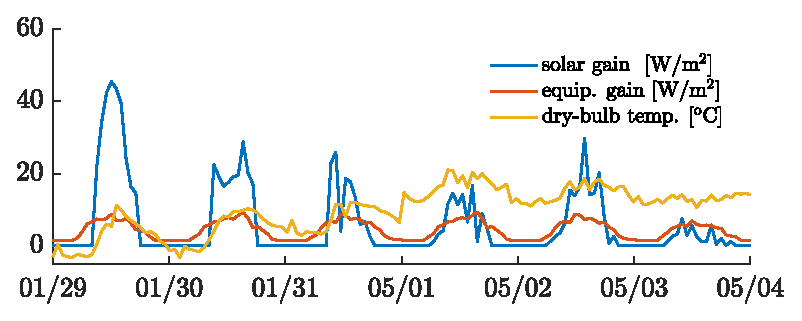
\includegraphics[width=25pc]{figures/disturbances.eps}
	}

	\subfigure[Optimal control input: cooling usage factor $\mathsf{C}$ with  $0 \leq \mathsf{C} \leq 1$. DPC-En generates a control strategy very simular to MPC.]{
		\label{F:control1}
		\centering
		\includegraphics[width=25pc]{figures/input3.eps}
	}

\end{center}
\end{figure}
\begin{figure}[h!]
\begin{center}
	\subfigure[Optimal control input: radiator heat $\mathsf{H}$ with  $0 \leq \mathsf{H} \leq 23 \ \mathrm{W/m^2}$. Again, DPC-En generates a control strategy very simular to MPC.]{
		\label{F:control2}
		\includegraphics[width=25pc]{figures/input4.eps}
	}

	\subfigure[Room temperature has time varying bounds. When the building is occuped the constraints are relaxed, else $19(20) \leq \mathsf{T}_{\mathrm{in}} \leq 25(26) \ \mathrm{^oC}$ in January(May). MPC and DPC-En are able to track the reference temperature ($22 \ \mathrm{^oC}$) closely.]{
		\label{F:state}
		\centering
		\includegraphics[width=25pc]{figures/state.eps}
	}

	\subfigure[Cumulative optimal cost after solving optimization. MPC serves as the benchmark with the minimum cost, followed by DPC-En and then DPC-RT.]{
		\label{F:obj}
		\centering
		\includegraphics[width=25pc]{figures/cumsumcost.eps}
	}
	\end{center}
	%\vspace{-1cm}
	\caption{Comparison of optimal performance obtained with MPC, DPC-En and DPC-RT for 3 days in January and 3 days in May.}
	\label{F:comparison}
	\captionsetup{justification=centering}
\end{figure}
Thus, we have shown that DPC-En provides a comparable performance to MPC without using the physical model.
However, one major limitation of the bilinear model is that the information about the building power consumption is not available. Much nonlinearities in the system are due to equipment efficiencies which are not considered in the bilinear case but are very important for practical purposes. 

Therefore, our next goal is to apply DPC-En on even more complex and realistic EnergyPlus model for which building a model predictive controller is time and cost prohibitive \cite{Sturzenegger2016}. This is because we would need to model intricate details like the geometry and construction layouts, the equipment design and layout plans, material properties, equipment and operational schedules etc.




\section{APPLICATION: DEMAND RESPONSE}
\label{S:casestudy}

In January 2014, the east coast (PJM) electricity grid experienced an 86x increase in the price of electricity from \$31/MWh to \$2,680/MWh in a matter of 10 minutes. Similarly, the price spiked 32x from an average of \$25/MWh to \$800/MWh in July of 2015. This extreme price volatility has become the new norm in our electric grids. Building additional peak generation capacity is not environmentally or economically sustainable. Furthermore, the traditional view of energy efficiency does not address this need for \emph{Energy Flexibility}. The solution lies with Demand Response (DR) from the customer side - curtailing demand during peak capacity for financial incentives. However, this is a very hard problem for commercial, industrial and institutional plants, the largest electricity consumers.
%the cost to model each building is over \$100K and buildings are all unique, they cannot decide which of the 100,000's of control knobs to turn as it is too complex, they must rely on rule-based curtailment approaches which are ad hoc, inefficient and do not provide any guarantees for energy reduction and are consequently exposed to a huge financial risk.

Thus, the problem of energy management during a DR event makes an ideal case for DPC. In the following sections, we apply DPC-En to a large scale EnergyPlus model to show how effectively DPC can provide a desired power curtailment as well as a desired thermal comfort. DPC builds predictive models of a building based on historical weather, schedule, set-points and electricity consumption data, while also learning from the actions of the building operator. These models are then used for synthesizing recommendations about the control actions that the operator needs to take, during a DR event, to obtain a given load curtailment while providing guarantees on occupant comfort and operations.

\subsection{EnergyPlus Model}
We use the DoE Commercial Reference Building (DoE CRB) simulated in EnergyPlus \cite{Deru2011} as the virtual test-bed building.
This is a large 6 story hotel building consisting of 22 zones with a total area of 122,120 sq.ft. 
During peak load conditions the building can consume up to 400 kW of power. 
For the simulation of the DoE CRB building we use actual meteorological year data from Chicago for the years 2012 and 2013. 

\subsection{Model training for DPC}

In the following simulations, we consider a long DR event from 7am - 2pm when the end-users are expected to follow/track the reference power signal sent by the utility. This is indeed common in Demand Tracking Control. 
During offline training, we sample data every 15 min to learn 2 kinds of forests. (1) Power forests are built using output as the total building power consumption, and (2) Temperature forests with output as temperature of one of the 22 zones. 

The training data set contains the following types of features. (1) The \textit{weather data} which includes measurements of the outside air temperature and relative humidity. Since we are interested in predicting the power consumption or the zone temperature for a finite horizon, we include the weather forecast of the complete horizon in the training features. (2) The \textit{schedule data} includes the proxy variables which correlate with repeated patterns of electricity consumption e.g., due to occupancy or equipment schedules. Day of Week is a categorical predictor which takes values from 1-7 depending on the day of the week. This variable can capture any power consumption patterns which occur on specific days of the week. Likewise, Time of Day is quite an important predictor of power consumption as it can adequately capture daily patterns of occupancy, lighting and appliance use without directly measuring any one of them. Besides using proxy schedule predictors, actual building equipment schedules can also be used as training data for building the trees. (3) The \textit{building data} include (i) cooling set points for  the guest rooms, kitchen and corridors, (ii) supply air temperature, and (iii) chilled water temperature.

For the following simulations, we use five control variables (i) cooling set point for corridors $\mathsf{ClgSP}$, (ii) cooling set point for guest rooms $\mathsf{GuestSP}$, (iii) cooling set point for kitchen $\mathsf{KitchenSP}$, (iv) chilled water supply temperature $\mathsf{ChwSP}$, and (v) supply air temperature  $\mathsf{SupplyAirSP}$, so $\tX^c = [\mathsf{ClgSP},\mathsf{GuestClgSP},\mathsf{KitchenClgSP},\mathsf{SupplyAirSP}, \mathsf{ChwSP}]$. 
The power forest $\mathcal{R}_p$ is built using the total building power consumption $\tP$. Its features $\tX^d$ include the weather variables, their lag terms and their forecast over the horizon, the schedule variables, and finally the lag terms of the power consumption.
The temperature forest $\mathcal{R}_t$ is built with zone temperature $\tT$ as the output. Except for the lag terms corresponding to the same zone temperature, all other features are same in $\tX^d$.

Fig.~\ref{F:sepvars} shows the prediction accuracy for the power forest, and also explains the two level training approach introduced in Sec.~\ref{SS:sepvar}. During S1, the forests are trained using only disturbances as the features. Then in S2, the local effects of the control variables are accounted for by the linear models in the leaves. We observe how the accuracy is drastically improved after including the linear models in the predictions.

\begin{figure}[h!]
	\centering
	\hspace{-0.3cm}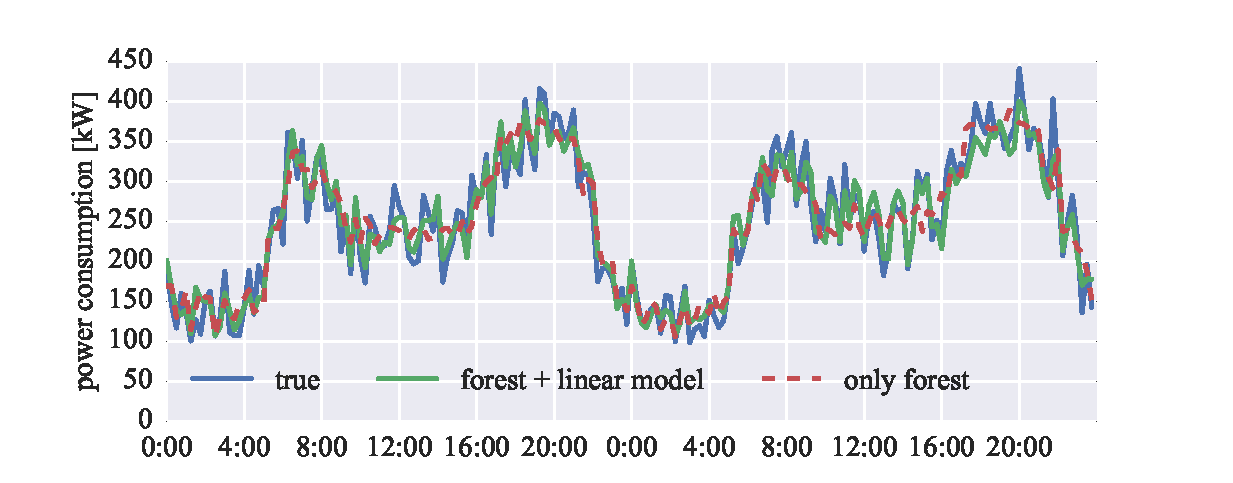
\includegraphics[width=22pc]{figures/eplus_validation.eps}	
	\caption{Model accuracy during training: The prediction made by forest using only $\tX^d$ (red) captures the effect due to disturbances. The linear models in the leaves capture the local effects (green) due to the control inputs $\tX^c$ and improve the model accuracy.}
	\label{F:sepvars}
	\captionsetup{justification=centering}
\end{figure}

\subsection{Power Management}
\label{SS:powermanagement}
Typically, the end customer receives a notification to curtail the power by some fraction. 
In this example on power management, we show how DPC can generate optimal inputs to track a desired power signal within a small allowance while maintaining the zone level thermal comfort. It may not be possible to have the same thermal comfort level in all the zones due to power curtailment, so we choose one zone (for example CEO's office) where the constraints must be met.
This is done by solving the following optimization problem with control variables $\tX^c = [\mathsf{ClgSP},\mathsf{GuestClgSP},\mathsf{KitchenClgSP},\mathsf{SupplyAirSP}, \mathsf{ChwSP}]$ as defined before:
\begin{align}
\begin{aligned}
\text{min } & \ \ \ \ \ \ \ \sum_{j=1}^{N} ({\tP}_{\mathrm{k+j|k}} - \tP_{\mathrm{ref}})^2 +  \lambda\epsilon_j + \nu \delta_j \\
\text{s.~t. } & \ \ \ \ \ \tP_{\mathrm{k+j|k}} =  \hat{\Theta}^T_{\tP_j} [ 1,\tX^c_{\mathrm{k|k}},\dots,\tX^c_{\mathrm{k+j-1|k}} ]^T \\
& \ \ \ \ \ \tT_{\mathrm{k+j|k}} =  \hat{\Theta}^T_{\tT_j} [ 1,\tX^c_{\mathrm{k|k}},\dots,\tX^c_{\mathrm{k+j-1|k}} ]^T \\
& \ \ \ \ \ \ \ \ \ \ \ \ \underline{\tP}-\epsilon_j \leq \tP_{\mathrm{k+j|k}} \leq \bar{\tP} + \epsilon_j\\
& \ \ \ \ \ \ \ \ \ \ \ \ \underline{\tT}-\delta_j \leq \tT_{\mathrm{k+j|k}} \leq \bar{\tT} + \delta_j\\
& \ \ \ \ \ \ \ \ \ \ \ \ \ \ \ \underline{\tX}^c \leq \tX^c_{\mathrm{k+j-1|k}} \leq \bar{\tX}^c\\ 
& \ \ \ \ \ \ \ \ \ \ \ \epsilon_j \geq 0,\delta_j \geq 0, \ j = 1,\dots,N.
\end{aligned}
\label{E:ptrack}
\end{align}

\begin{figure}[h]
	\subfigure[Optimal inputs calculated by DPC-En. At first, the inputs are changed rapidly because of a significant difference between the desired and the actual power consumption. Then gradual adjustments are made to follow the desired reference.]{
		\label{F:eplus_inputs}
		\centering
		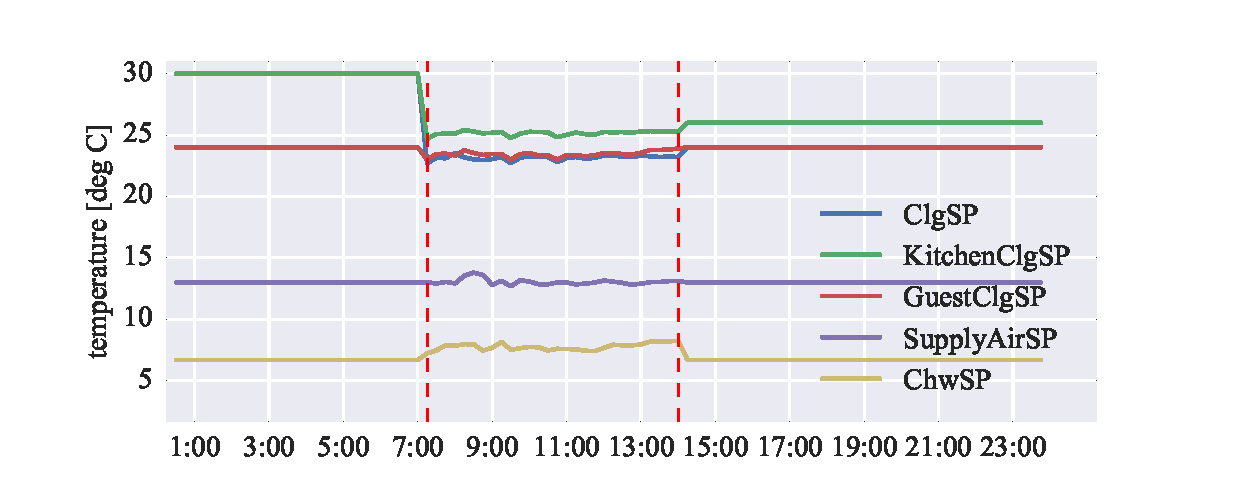
\includegraphics[width=22pc]{figures/eplus_control.eps}
	}
	\subfigure[Power tracking by DPC-En at 1.1 MW: The difference in closed-loop simulation and prediction is due to model mismatch.]{
		\label{F:eplus_power}
		\centering
		\includegraphics[width=22pc]{figures/eplus_closedloop.eps}
	}
	\caption{Power management using DPC. The controller is active between 7am - 2pm. This region is marked in dashed red lines.}
	\captionsetup{justification=centering}
	\label{F:eplus_track}
\end{figure}

Here, the temperature forests are used to enforce thermal constraints in the zone of interest. The setup of optimization problem is flexible to include even other variables in the cost or the constraints. For example, we are currently looking at including the dynamic pricing of electricity in the cost since the customers can more directly relate to the financial incentives.

The results are shown in Fig.~\ref{F:eplus_track}. 
The DPC controller is active between 7am - 2pm. Before 7am and after 2pm, the building is using a predefined rule-based control strategy.
The optimal control inputs from DPC-En are shown in Fig.~\ref{F:eplus_inputs}. It is observed that, with the optimal inputs generated by DPC, we can track the reference power consumption signal closely. In fact, the average tracking error between 7am - 2pm is 3\%. The difference between the predicted power consumption and that in the closed-loop simulation in Fig.~\ref{F:eplus_power} is due to model mismatch between the EnergyPlus model and the power forest used in the optimization \eqref{E:ptrack}. Due to this inaccuracy, the actual power consumption is on an average 7 kW higher.

Thus, DPC-En successfully tracks a given power reference signal with an average $\sim$ 3\% error for such a complex building which would require several years of efforts to develop a physics based model.




\subsection{Practical Challenges and Future Work}
\label{SS:challenges}
\begin{enumerate}
\item \emph{\textbf{Data Availability:}} The main practical challenge for DPC lies in the availability of data for training, and we require answers to questions like \emph{how much data (functional testing) is required, and how should the sampling be done?} Therefore, the procedure for optimal experiment design, and model improvement with estimation of variance in predictions is one of the main focus of our ongoing work.
\item \emph{\textbf{Stability:}} While the buildings are inherently stable, many other applications require stability guarantees. In our ongoing work, we are working towards proving asymptotic stability to origin with DPC-RT and DPC-En by using concept of switched LTI systems. This will make DPC useful for systems with faster dynamics.
\end{enumerate}


\section{CASE STUDY: OPTIMAL HEATING SYSTEM SCHEDULING}
\label{S:realCaseStudy}

In this section, we show an application of DPC to a real house located in L'Aquila, Italy. Random forest models for DPC built using historical data from this house are described in Section \ref{SS:randomForestsModels}. 
In Section \ref{SS:energyPlusmodel}, we present the thermal energy model of the building in EnergyPlus, built using historical data, construction layout and materials after spending $\sim3$ months of efforts.
In Section \ref{SS:controllersDPCandBangbang}, we set up the DPC optimization problem and describe the bang-bang control strategy.
Finally, in Section \ref{SS:simulationResults}, the performance of the two controllers are compared in terms of energy saving using the EnergyPlus model.
\textcolor[rgb]{0,0,1}{In particular, in Section \ref{SSS:DisturbancePerfect}, we show that DPC allows an energy saving up to $49.2\%$ with respect to the bang-bang controller while guaranteeing thermal comfort for occupants, considering the perfect knowledge of the weather forecast. 
In Section \ref{SSS:DisturbanceUncertain}, we show that DPC is robust with respect to imperfect weather forecast.}
The section organization is graphically shown in Figure \ref{F:overview}.
\begin{figure}[h!]
	\begin{center}
		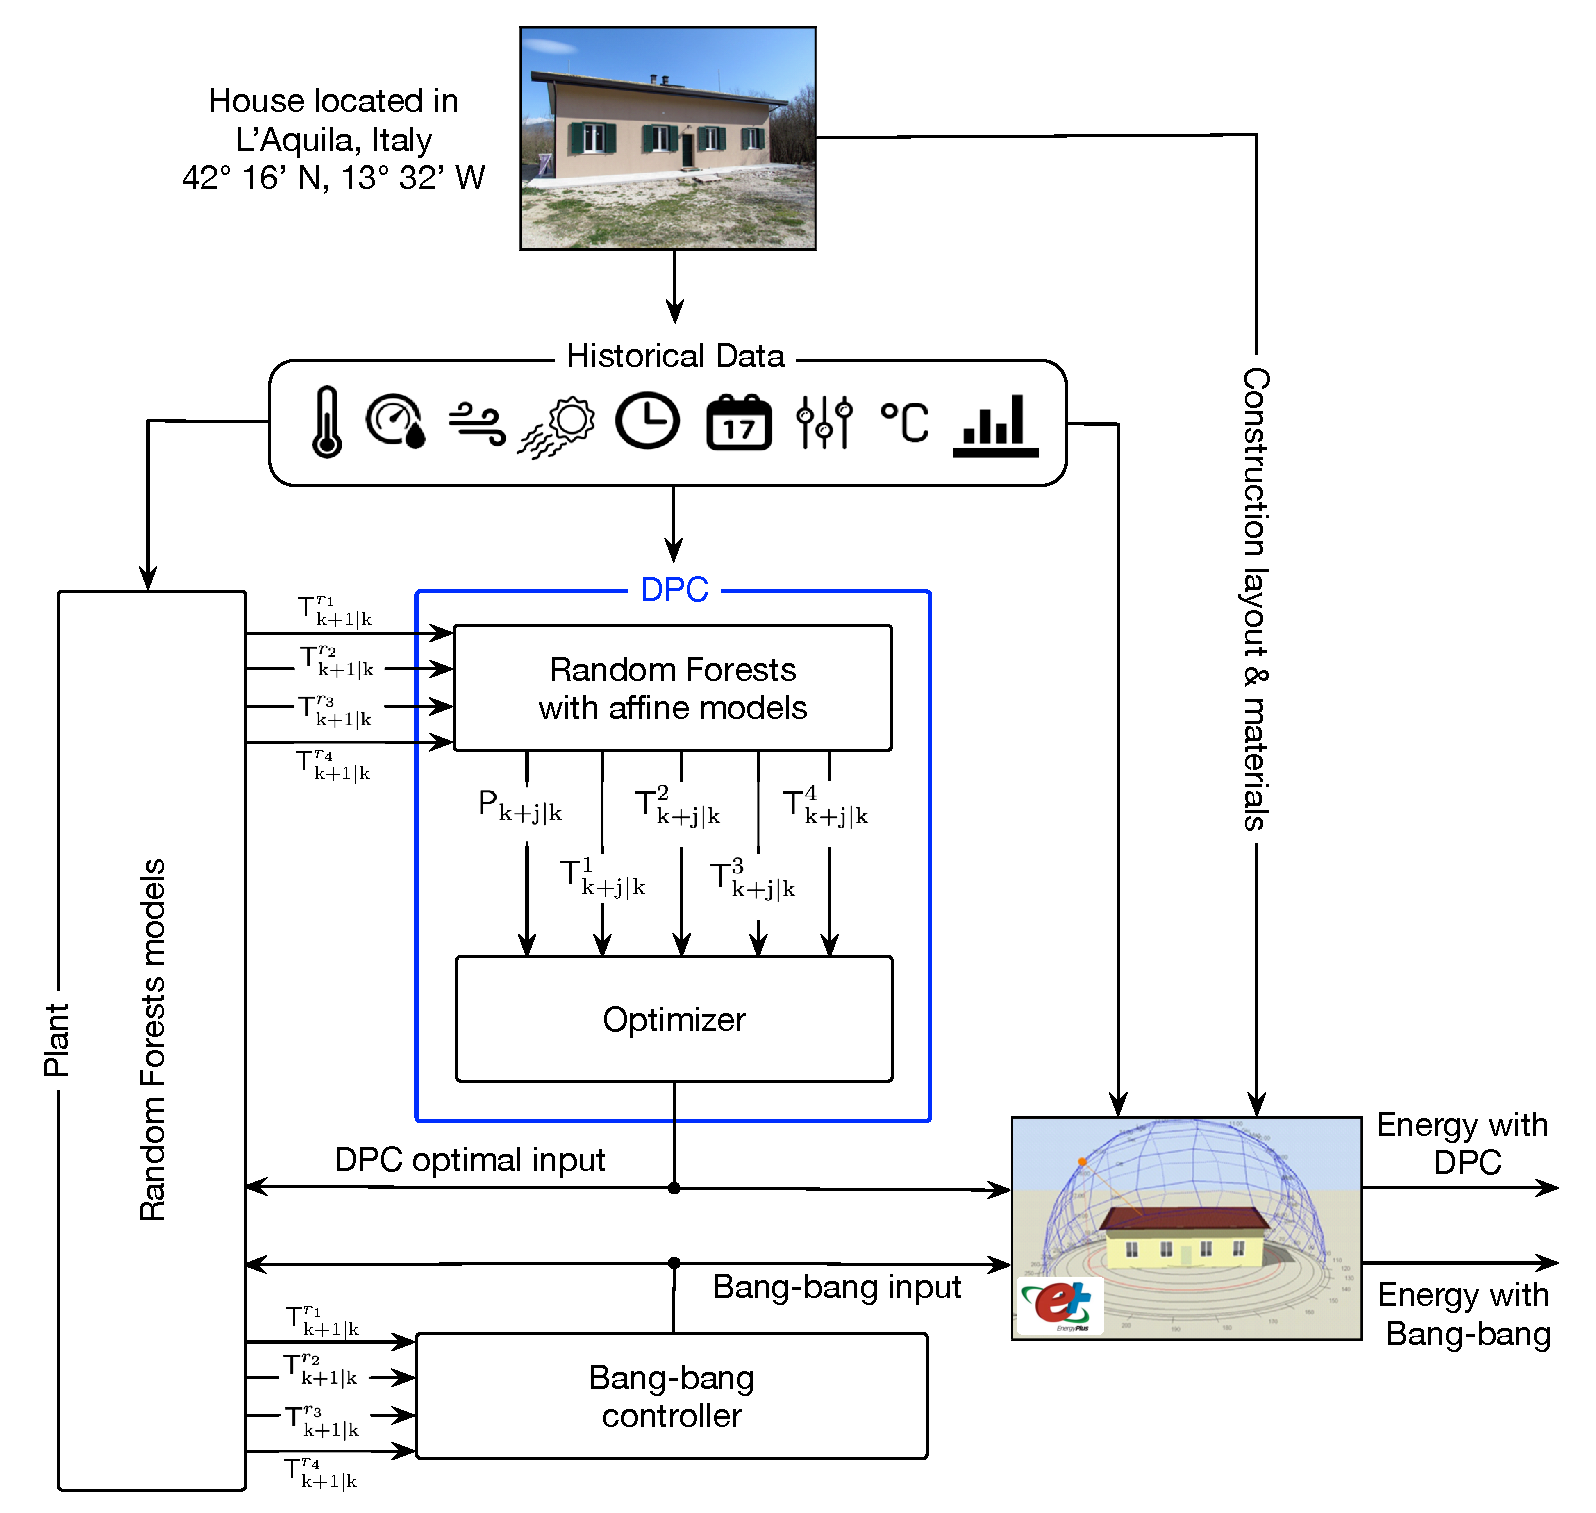
\includegraphics[width=1\linewidth]{figures/overview.eps}
		\caption{Random Forest trained on all features including the control variable are used as the plant in the closed-loop simulations with DPC and bang-bang controller. DPC optimzation uses Random Forests with affine functions as predictive models. Controllers' strategies are evaluated using the EnergyPlus model to compare the actual energy consumption.}
		\captionsetup{justification=centering}
		\label{F:overview}
	\end{center}
\end{figure}

\textcolor[rgb]{0,0,1}{The contribution of this section with respect to Sections \ref{S:casestudy} is threefold:
\begin{enumerate}
	\item we consider experimental data from a lived house, hence subject to real world imperfections, such as random (non predictable) occupancy schedules, open/close windows, random (non predictable) light on/off switch, etc..
	On the other hand, the EnergyPlus model considered in Section \ref{S:casestudy}, although provides an accurate model of a building, is still a simulated model that does not take into account the aforementioned imperfections;
	\item we modify the DPC algorithm to take into account uncertainties on the weather forecast, so making DPC robust with respect to prediction errors;
	\item in Section \ref{S:casestudy}, we want to cut the peak of the power in a specific time range while keeping the temperature as close as possible to a specific setpoint.
	Differently, in this section, we show the adaptability of DPC to different problems, minimizing the energy consumption required to keep room temperatures within a specified range of comfort for an arbitrary amount of time. In this way we show the potential of DPC for energy saving on a long period. 
\end{enumerate}}
\subsection{Description of the house}\label{SS:descriptionHouse}
The chosen case study is a detached off-grid two-story residential house, located in the outskirt of L'Aquila (coordinates $42\degree$ $16'$ latitude and $13\degree$ $32'$ longitude), Italy and is shown in Figure \ref{F:house}. The building, inhabited by the two owners, has a main north-south orientation and it is composed by a heated ground floor and an attic without heating system. Therefore, although the gross area of the house is equal to $209.5\,m^2$, the heated gross area is equal to $112.4\,m^2$.
Thanks to the off-grid characteristic, the technological plants guarantee the complete energy self-sufficiency of the building. The house is equipped with a biomass boiler, a solar thermal plant, a stand-alone photovoltaic system, black water and rainwater reuse systems and a well for water supply, and has complete independence from the utilities.   
The bearing structure of the house is made of reinforced concrete and EPS (expanded polystyrene) insulation, while the building envelope is composed by prefabricated wood-cement blocks, shown in Figure \ref{F:houseSection}, with EPS and graphite insulation, that allow low thermal fluxes. The thermal performance of a wood-cement block, with similar geometry, was investigated in a previous work \cite{Nardi2016}, both with experimental and numerical approach.
The heating system of the building, that supplies the thermal energy required in winter season, is a hydronic system consisting of a vegetable biomass boiler, with a manual ON/OFF, a constant-flow pump station, and tubular steel radiators as shown in Figure \ref{F:housePlantScheme}. The standard biomass boiler has an efficiency of $83.5\%$ with $16.5\ kW$ of thermal power transferred to the water, without gas-flame modulation. The heat transfer fluid distribution is realized through a manifold circuit, that supplies the radiators placed in the various rooms of the house. The energy needs for the domestic hot water (DHW) are covered by the same boiler, coupled with a solar thermal plant. It is worth noting that, in this work, the thermal energy needed for the domestic hot water production is neglected. 
\begin{figure}[t!]
	\begin{center}
		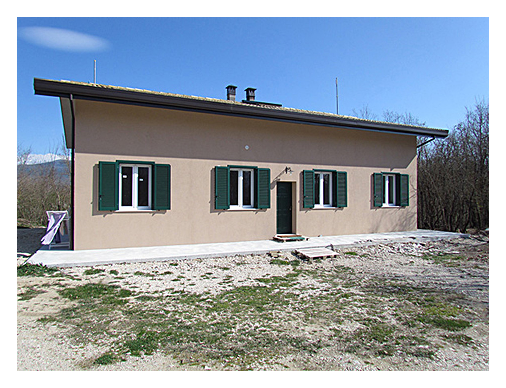
\includegraphics[width=20pc]{figures/Vista_sud.eps}
		\caption{Off-grid residential house.}
		\captionsetup{justification=centering}
		\label{F:house}
	\end{center}
%	\vspace{-0.5cm}
\end{figure}
\begin{figure}[h!]
	\begin{center}
		\subfigure[Walls.]{
			\label{F:houseSection1}
			\centering
			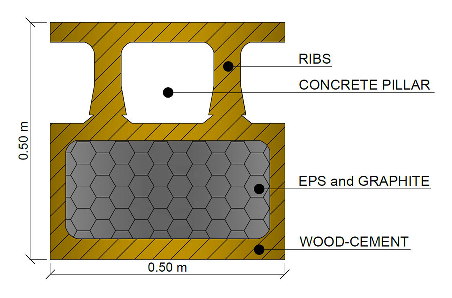
\includegraphics[width=16pc]{figures/blocco_parete_rev01.eps}
		}
		\subfigure[Floor and roof.]{
			\label{F:houseSection2}
			\centering
			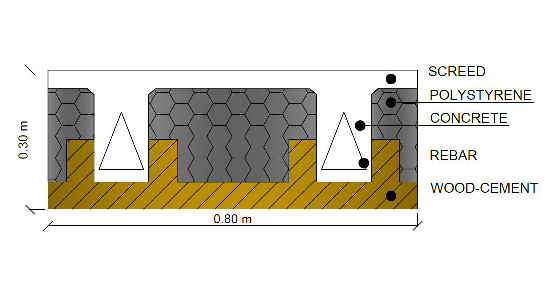
\includegraphics[width=17pc]{figures/blocco_solaio_rev01.eps}
		}
	\end{center}
	\vspace{-0.5cm}
	\caption{Cross-sections of the wood-cement blocks.}
	\captionsetup{justification=centering}
	\label{F:houseSection}
\end{figure}
For a thorough knowledge of the building thermal behavior, an in-situ analysis was carried out. Temperature measuring devices, completely self-produced at the “G. Parolini Lab” of the University of L'Aquila \cite{Pantoli2017}, mainly based on an $ATmega 2560$ microcontroller and $DS18B20$ temperature probes (temperature range from $-55.0\degree C$ to $125.0\degree C$ with an accuracy of $\pm 0.5\degree C$), were employed to acquire the ambient temperatures of $4$ differently oriented rooms of the house as shown in Figure \ref{F:houseFloors} (displayed with red dots $A1$, $A2$, $A3$ and $A4$). The probes positions were chosen to optimize the data acquisition and to minimize the discomfort of the occupants in the house. Furthermore, as can be seen in Figures \ref{F:housePlantScheme} and \ref{F:houseFloors}, a commercial heat meter (temperature range from $10.0\degree C$ to $90.0\degree C$ with an accuracy of $\pm 0.05\degree C$, displayed with orange dot $G1$) was installed downstream of the biomass boiler to measure the produced thermal energy. The turbine flowmeter was installed on the return pipe, while the two thermocouples were placed inside the delivery and return pipes, respectively. All the measuring devices have been set with a data acquisition rate equal to $10$ minutes, from March $11^{th}$ $2016$ to May $15^{th}$ $2016$.

The collected data are used in the following to create both an EnergyPlus and a random forest model for the energy consumption assessment of the house. These models will be used for performance comparison of DPC with respect to a classical bang-bang controller. In particular DPC will be set up to provide an optimal ON/OFF scheduling policy for the heating system in order to save energy while guaranteeing thermal comfort for the occupants. To this aim, we also create random forest models for power consumption and room temperatures to be used in the closed-loop simulations. 

\begin{figure}[t!]
	\begin{center}
		\includegraphics[width=27pc]{figures/Schema_di_impianto.eps}
		\caption{Technological plant scheme of the use case.}
		\captionsetup{justification=centering}
		\label{F:housePlantScheme}
	\end{center}
\end{figure}
\begin{figure}[t!]
	\begin{center}
		\subfigure[Ground floor.]{
			\label{F:houseGroundFloor}
			\centering
			\includegraphics[width=26pc]{figures/Arch_PT_e_sonde.eps}
		}
		\subfigure[Attic.]{
			\label{F:houseAttic}
			\centering
			\hspace{-1.6cm}
			\includegraphics[width=22.8pc]{figures/Arch_P1.eps}
		}
	\end{center}
	\caption{Layout of the house and probes placement. Legend: red circle for ambient temperature; orange circle for heat meter.}
	\captionsetup{justification=centering}
	\label{F:houseFloors}
\end{figure}
\subsection{EnergyPlus model}\label{SS:energyPlusmodel}
In this section we create an EnergyPlus model of the thermal energy consumption of the house that will be used in Section \ref{SS:simulationResults} to compare the quality of the DPC with respect to a classical bang-bang controller.

To assess energy performance of the use case heating system, the EnergyPlus \cite{energyPlus} together with DesignBuilder modeling environment \cite{designBuilder} has been employed. The model has been created based  on L'Aquila weather data, shown in Figure \ref{F:houseExternalWeather}, provided by the CETEMPS – Centre of Excellence \cite{CETEMPS}. According to the K\"{o}ppen-Geiger climate classification, Italy is classified in Csa, Cfa and Csb climate zones, with a warm temperate climate \cite{Peel2007}.

Because of the complex morphology of the blocks shown in Figure \ref{F:houseSection}, some simplified assumptions were made, in order to create the EnergyPlus virtual model. Considering the thermal properties of the wood-cement blocks that compose the walls shown in Figure \ref{F:houseSection1}, the thermal effects of the ribs were neglected. For the block employed for floor and roof shown in Figure \ref{F:houseSection2}, a less complex equivalent block, with only three layers, was evaluated in order to consider only one equivalent thermal transmittance value. The properties of the blocks used for the simulation model are listed in Table \ref{T:houseProperties}.    

Therefore, the dynamic simulation model of the use case, shown in Figure \ref{F:houseVirtualModel}, has been created by analyzing the fundamental characteristics of the building (orientation, geometry, structural members, heating system components, air changes with natural ventilation, activity, internal gains, air leakages) and the weather file specifically created for L'Aquila. The comprehensive method was chosen for modeling the heating system, once checked all the characteristics of the components.
\begin{figure}[t!]
	\begin{center}
		\hspace{-0.7cm}
		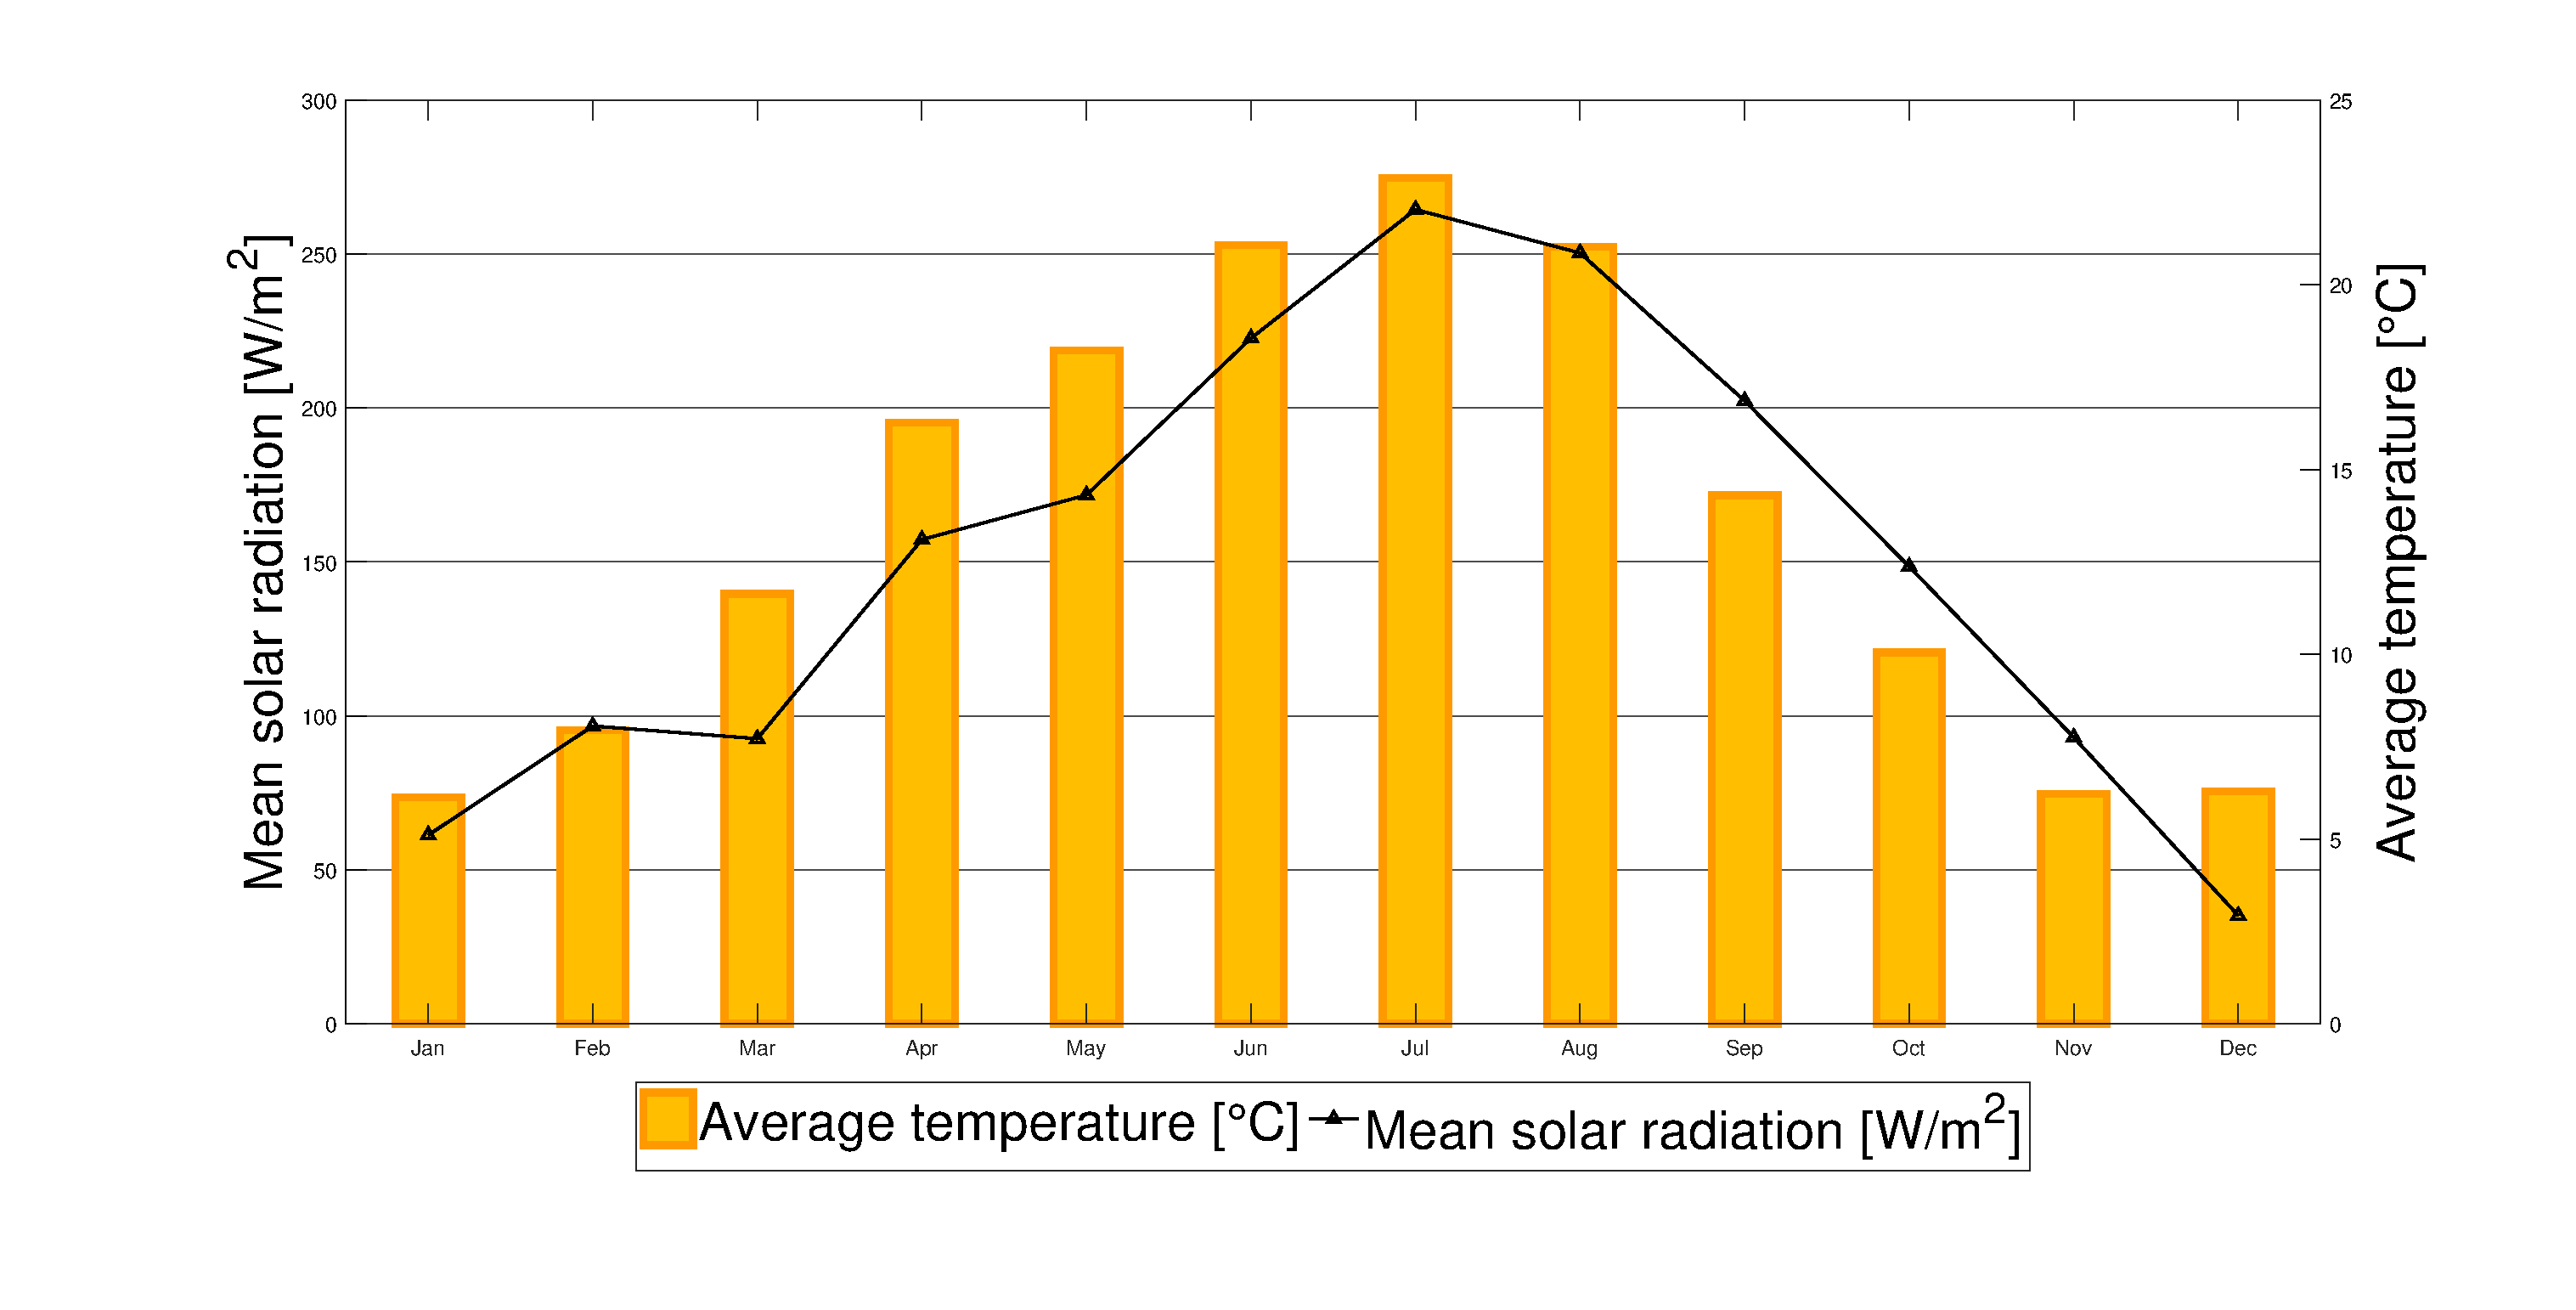
\includegraphics[width=28pc]{figures/dati_climatici_rev01.eps}
		\vspace{-0.5cm}
		\caption{Weather data of L'Aquila, Italy.}
		\captionsetup{justification=centering}
		\label{F:houseExternalWeather}
	\end{center}
\end{figure}
\begin{table}[t!]
	\centering
	\begin{tabular}{ccccc}
		\toprule
		\multirow{3}{1.4cm}{\centering Structural member} & \multirow{3}{3.7cm}{\centering Layer 
			description (from inside to outside)}       & Thermal     		     & Total     & Total        \\
		&                                             & resistance   		     & thickness & U-value      \\
		&                                             & $[(m^2K)/W]$		     & $[m]$     & $[W/(m^2K)]$ \\
		
		
		\midrule
		\multirow{3}*{Wall}                               & Wood-cement                                 & $0.308$     		     &           &              \\ 
		& Concrete                                    & $0.096$    		     & $0.50 $   & $0.12 $      \\ 
		& EPS and graphite                            & $6.774$    		     &           &              \\
		&							                    &						 &		     &			    \\
		
		
		\multirow{3}*{Floor}        					  & Wood-cement                                 & $0.308$     		     &           &              \\ 
		& Polystyrene                                 & $6.000$     		     & $0.23 $   & $0.28 $      \\ 
		& Screed                                      & $0.027$     		     &           &              \\
		&									    	    &					 	 &		     &			    \\
		
		
		\multirow{5}{1.4cm}{\centering Pitched roof} 	  & Wood-cement                                 & $0.308$                &           &              \\ 
		& Polystyrene                                 & $6.000$                &           &              \\
		& Screed                                      & $0.027$                & $0.31 $   & $0.13 $      \\ 
		& \multirow{2}{3.7cm}{\centering Polyurethane 
			resins and polyisocianurate foams}          & \multirow{2}*{$4.000$} &           &              \\
		&                                             &                        &           &              \\
		\bottomrule
	\end{tabular}
	\caption{Wood-cement blocks properties.}
	\captionsetup{justification=centering}
	\label{T:houseProperties}
\end{table}
In order to calibrate the EnergyPlus model, a comparison between simulated and measured thermal energy consumption was performed. Considering the off-grid characteristic of the house, the installation of a heat meter was necessary for acquiring the actual energy consumption. Moreover, the heat meter installation has allowed a detailed knowledge of the actual heating system scheduling, shown in Figure \ref{F:houseActualScheduling}, faithfully reproduced in the simulated model. The heat meter, that consists of two thermocouples for flow and return thermal fluid temperatures, a turbine flowmeter and a controller, employed Equation \eqref{Eq:energyConsumption} to calculate the real thermal energy consumption $\dot Q$ of the house.
\begin{equation}\label{Eq:energyConsumption}
\dot Q = 0.2777698\times10^{-3}\times\rho\times\Delta V\times c_p\times\Delta T
\end{equation}
In \eqref{Eq:energyConsumption} $\dot Q$ is the thermal energy consumption $[Wh]$, $\rho$ is the water density $[kg/m^3]$, $\Delta V$ is the water volume variation $[m^3]$ detected by the turbine flowmeter, $c_p = 4.186\, [kJ/(kgK)]$ is the water specific heat at constant pressure, $\Delta T$ is the difference between flow and return temperatures of the water $[K]$, $0.2777698∙10−3$ is a dimensionless conversion factor. The considered period goes from March $15$, $2016$ to April $15$, $2016$.
\begin{figure}[t!]
	\begin{center}
		\includegraphics[width=20pc]{figures/Render_rev01.eps}
		\caption{Virtual model of the use case.}
		\captionsetup{justification=centering}
		\label{F:houseVirtualModel}
	\end{center}
\end{figure}
\begin{figure}[t!]
	\begin{center}
		\includegraphics[width=28pc]{figures/Scheduling_rev02.eps}
		\caption{Actual scheduling of the heating system, where white color means switched OFF and green color switched ON, and ($T_{ext,ave}$) is the external average temperature. From midnight to $8am$ the heating system is always switched off.}
		\captionsetup{justification=centering}
		\label{F:houseActualScheduling}
	\end{center}
\end{figure}
Following the hourly calibration proposed by the M\&V guidelines of ASHRAE \cite{USDOE}, also applied in \cite{Mustafarai2014,Raftery2011}, a simulated model is calibrated when the mean bias error (MBE) and the coefficient of variation of the root mean square error [CV(RMSE)] are less than acceptable tolerances, respectively equal to $\pm 10.0\%$ and $30.0\%$. MBE and CV(RMSE) have been calculated by using Equations \eqref{Eq:mbe} and \eqref{Eq:cvrmse}.

\begin{equation}\label{Eq:mbe}
MBE(\%) = \frac{\sum_{Period}{(S-M)_{Interval}}}{\sum_{Period}{M_{Interval}}} \times 100
\end{equation}

where $M$ is the measured $kWh$ and $S$ is the simulated $kWh$.

\begin{align}\label{Eq:cvrmse}
\nonumber CV(RMSE_{Period}) &= \frac{RMSE_{Period}}{A_{Period}} \times 100 \\
				            &= \sqrt{\frac{\sum{(S-M)^2_{Interval}}}{N_{Interval}}} \times \frac 1{A_{Period}} \times 100
\end{align}

where $A_{Period}$ is the mean of the measured data for the period, Equation \eqref{Eq:aperiod}, and $N_{Interval} = 4563$ is the number of time intervals in the monitoring period.

\begin{equation}\label{Eq:aperiod}
A_{Period} = \frac{\sum_{Period}{M_{Interval}}}{N_{Interval}}
\end{equation}

The comparison between numerical and experimental data is shown in Figure \ref{F:houseComparisonExperimental} and shows a quite good agreement. Therefore, with a MBE equal to $7.38\%$ and a CV(RMSE) equal to $8.37\%$, the EnergyPlus model of the use case can be considered well calibrated.  
\begin{figure}[t!]
	\begin{center}
		\subfigure[Thermal energy comparison. The accuracy error is $7.38\%$ with MBE definition and $8.37\%$ with CV(RMSE) definition]{
			\label{F:houseComparisonExperimentalEnergy}
			\centering
			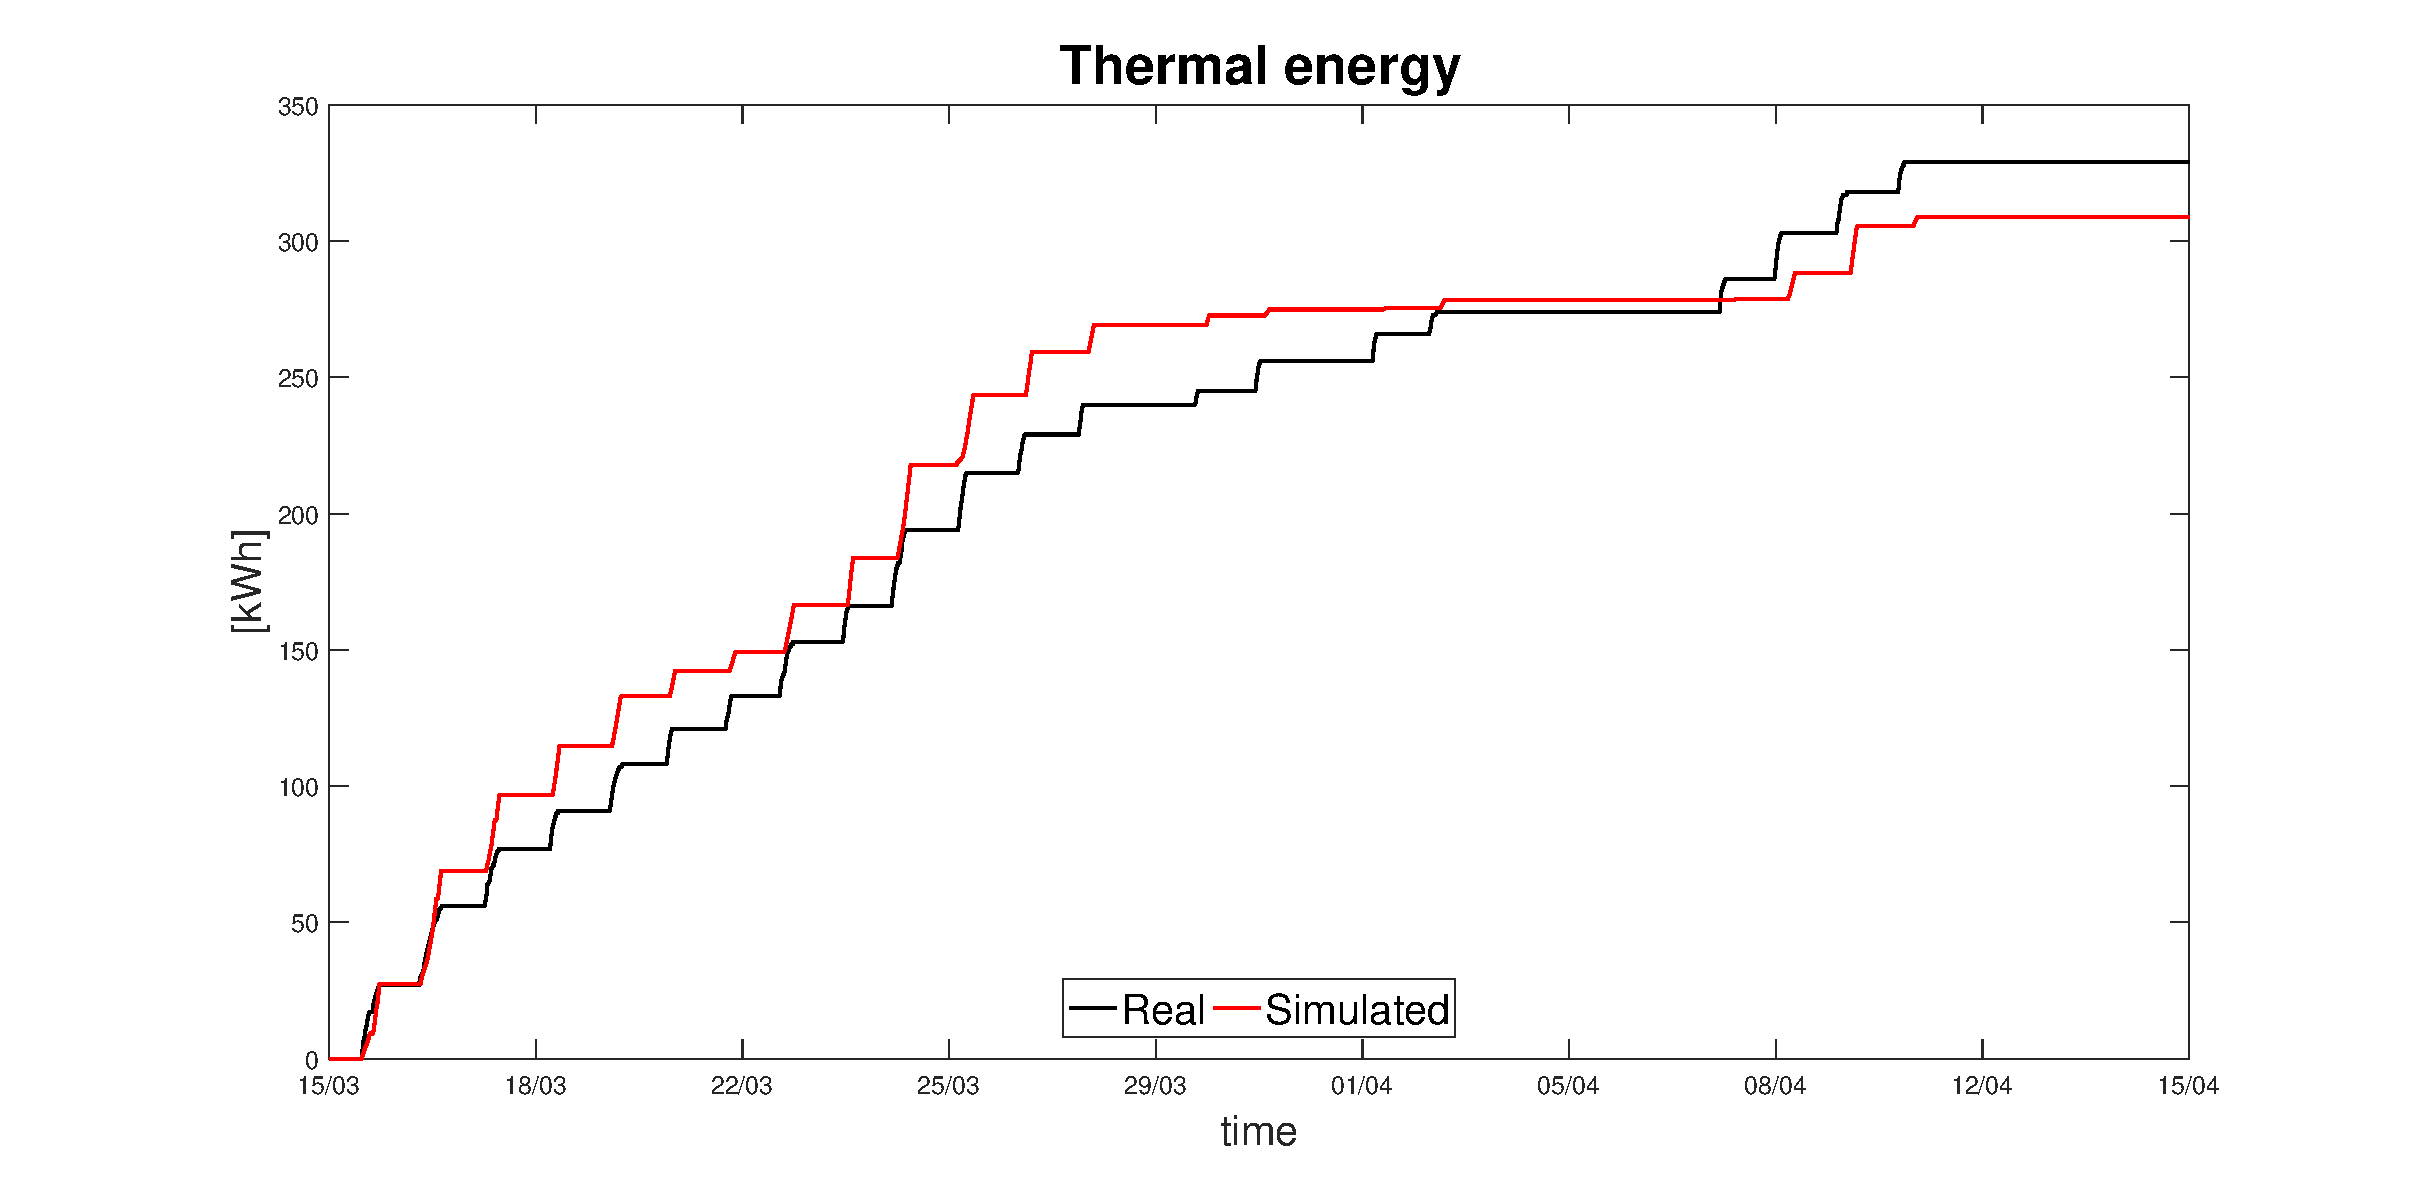
\includegraphics[width=28pc]{figures/Thermal_energy_rev01.eps}
		}
		\subfigure[Thermal power comparison.]{
			\label{F:houseComparisonExperimentalPower}
			\centering
			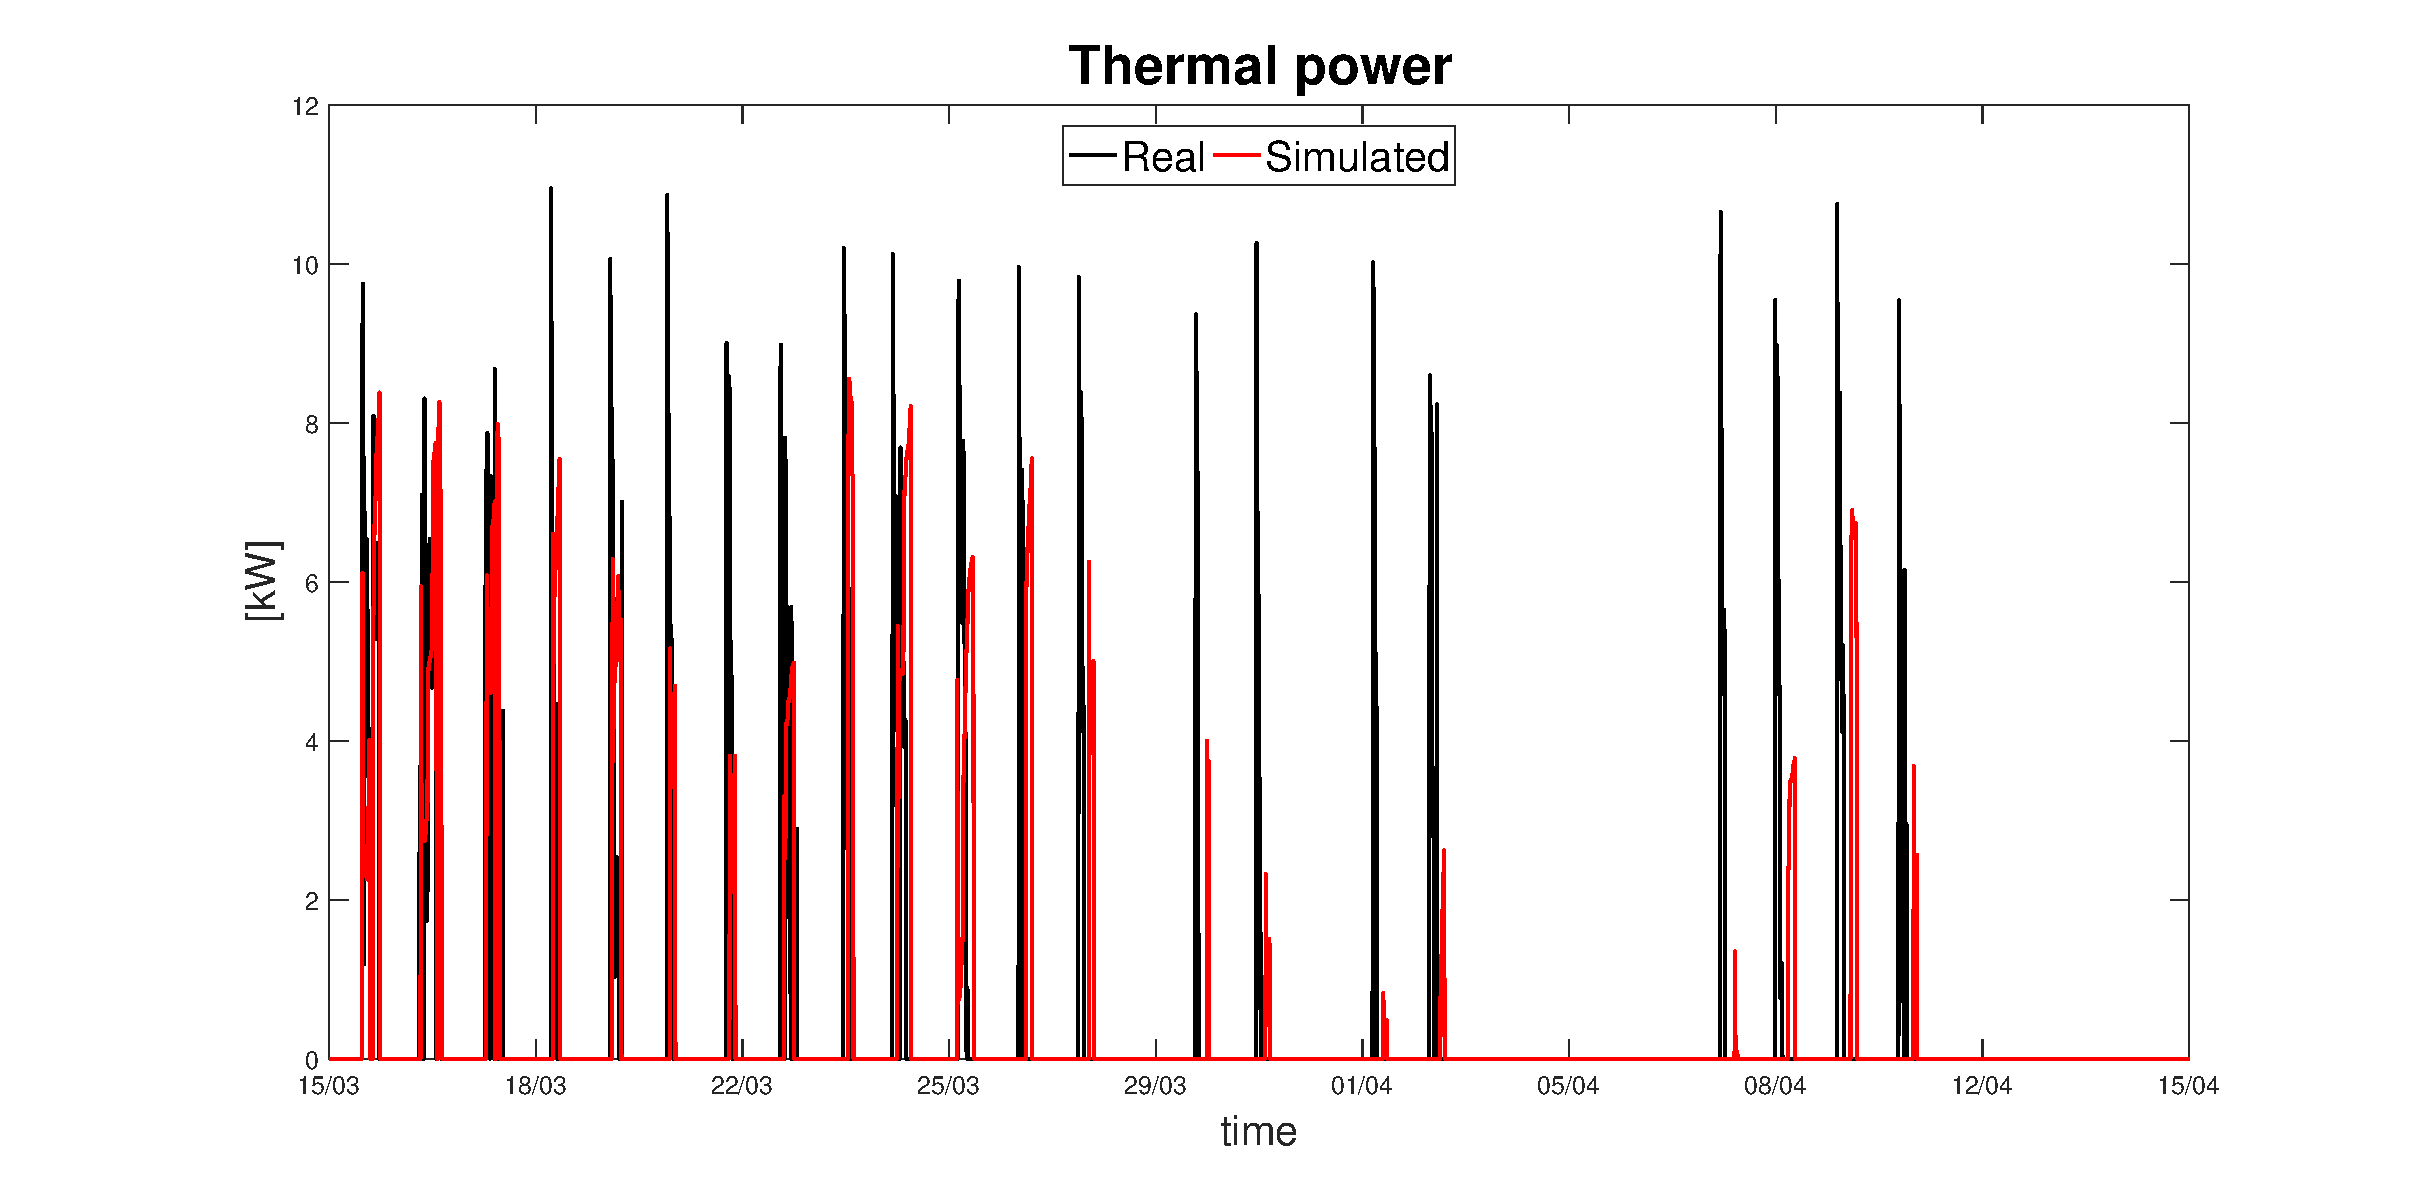
\includegraphics[width=28pc]{figures/Thermal_power.eps}
		}
	\end{center}
	\caption{Comparison between numerical and experimental data.}
	\captionsetup{justification=centering}
	\label{F:houseComparisonExperimental}
\end{figure}
\subsection{Random forest models}
\label{SS:randomForestsModels}
For the closed-loop simulations with DPC we create $2$ different sets of models, $S_1 = \{\tT^{r_1}_{k+j},\tT^{r_2}_{k+j},\tT^{r_3}_{k+j},\tT^{r_4}_{k+j}\}$ and $S_2 = \{\tP_{k+j},\tT^{1}_{k+j},\tT^{2}_{k+j},\tT^{3}_{k+j},\tT^{4}_{k+j},\ j = 1,\ldots,N\}$, using random forests. In each set we have  $4$ models that describe the room temperature evolution ($\tT^{r_i}$ and $\tT^i$, $i=1,2,3,4$) in each of the $4$ rooms equipped with temperature sensors. In $S_2$ we have a model for the power consumption of the house ($\tP$). Models in $S_1$ are created using the classical random forests algorithm with all the features and are used as plant simulator of the house. For this reason, they are computed to give prediction only for time step $k+1$ and not over the whole horizon $N$. Models in $S_2$ are used as predictors over a horizon $N$ in the DPC algorithm and are then created using the methodology provided in Section \ref{SS:dpcrf}. The non-manipulated features in $\X^d$ are the disturbance data (relative humidity, atmospheric pressure, outside air temperature, solar radiation, wind, time of the day and day of the week) and the states (temperature of the $4$ rooms). The manipulated feature in $\X^c$ is the flow rate ($[m^3/h]$). All this features are used to create models in $S_1$ and the power model in $S_2$, while disturbance data, state temperature of room $i$ only and flow rate are used to identify $\hat{\Theta}_{\tT^i_j}$ for temperature models in $S_2$. All the models have been trained on the data from March $11$, $2016$ to April $26$, $2016$ and validated on the data from May $1$, $2016$ to May $15$, $2016$. The accuracy of these models with respect to real data is shown in Table \ref{T:S1accuracy}, based on the definition of Normalized Root Mean Square Error (NRMSE).

A graphical comparison is shown in Figure \ref{F:power_testing} for the power consumption and Figure \ref{F:temperature_testing} for the temperature of room $1$. The plots for the other rooms are omitted since they are very similar.


%We use random forest model $\tP^r$ also to estimate the energy consumption of the house. In particular we estimated it for the same period analyzed in Section \ref{SS:energyPlusmodel} and obtained the results in Figure \ref{F:Energy_testing}, with a MBE equal to $13.0\%$ and a CV(RMSE) equal to $13.7\%$.
%
%\begin{figure}[h!]
%	\begin{center}
%		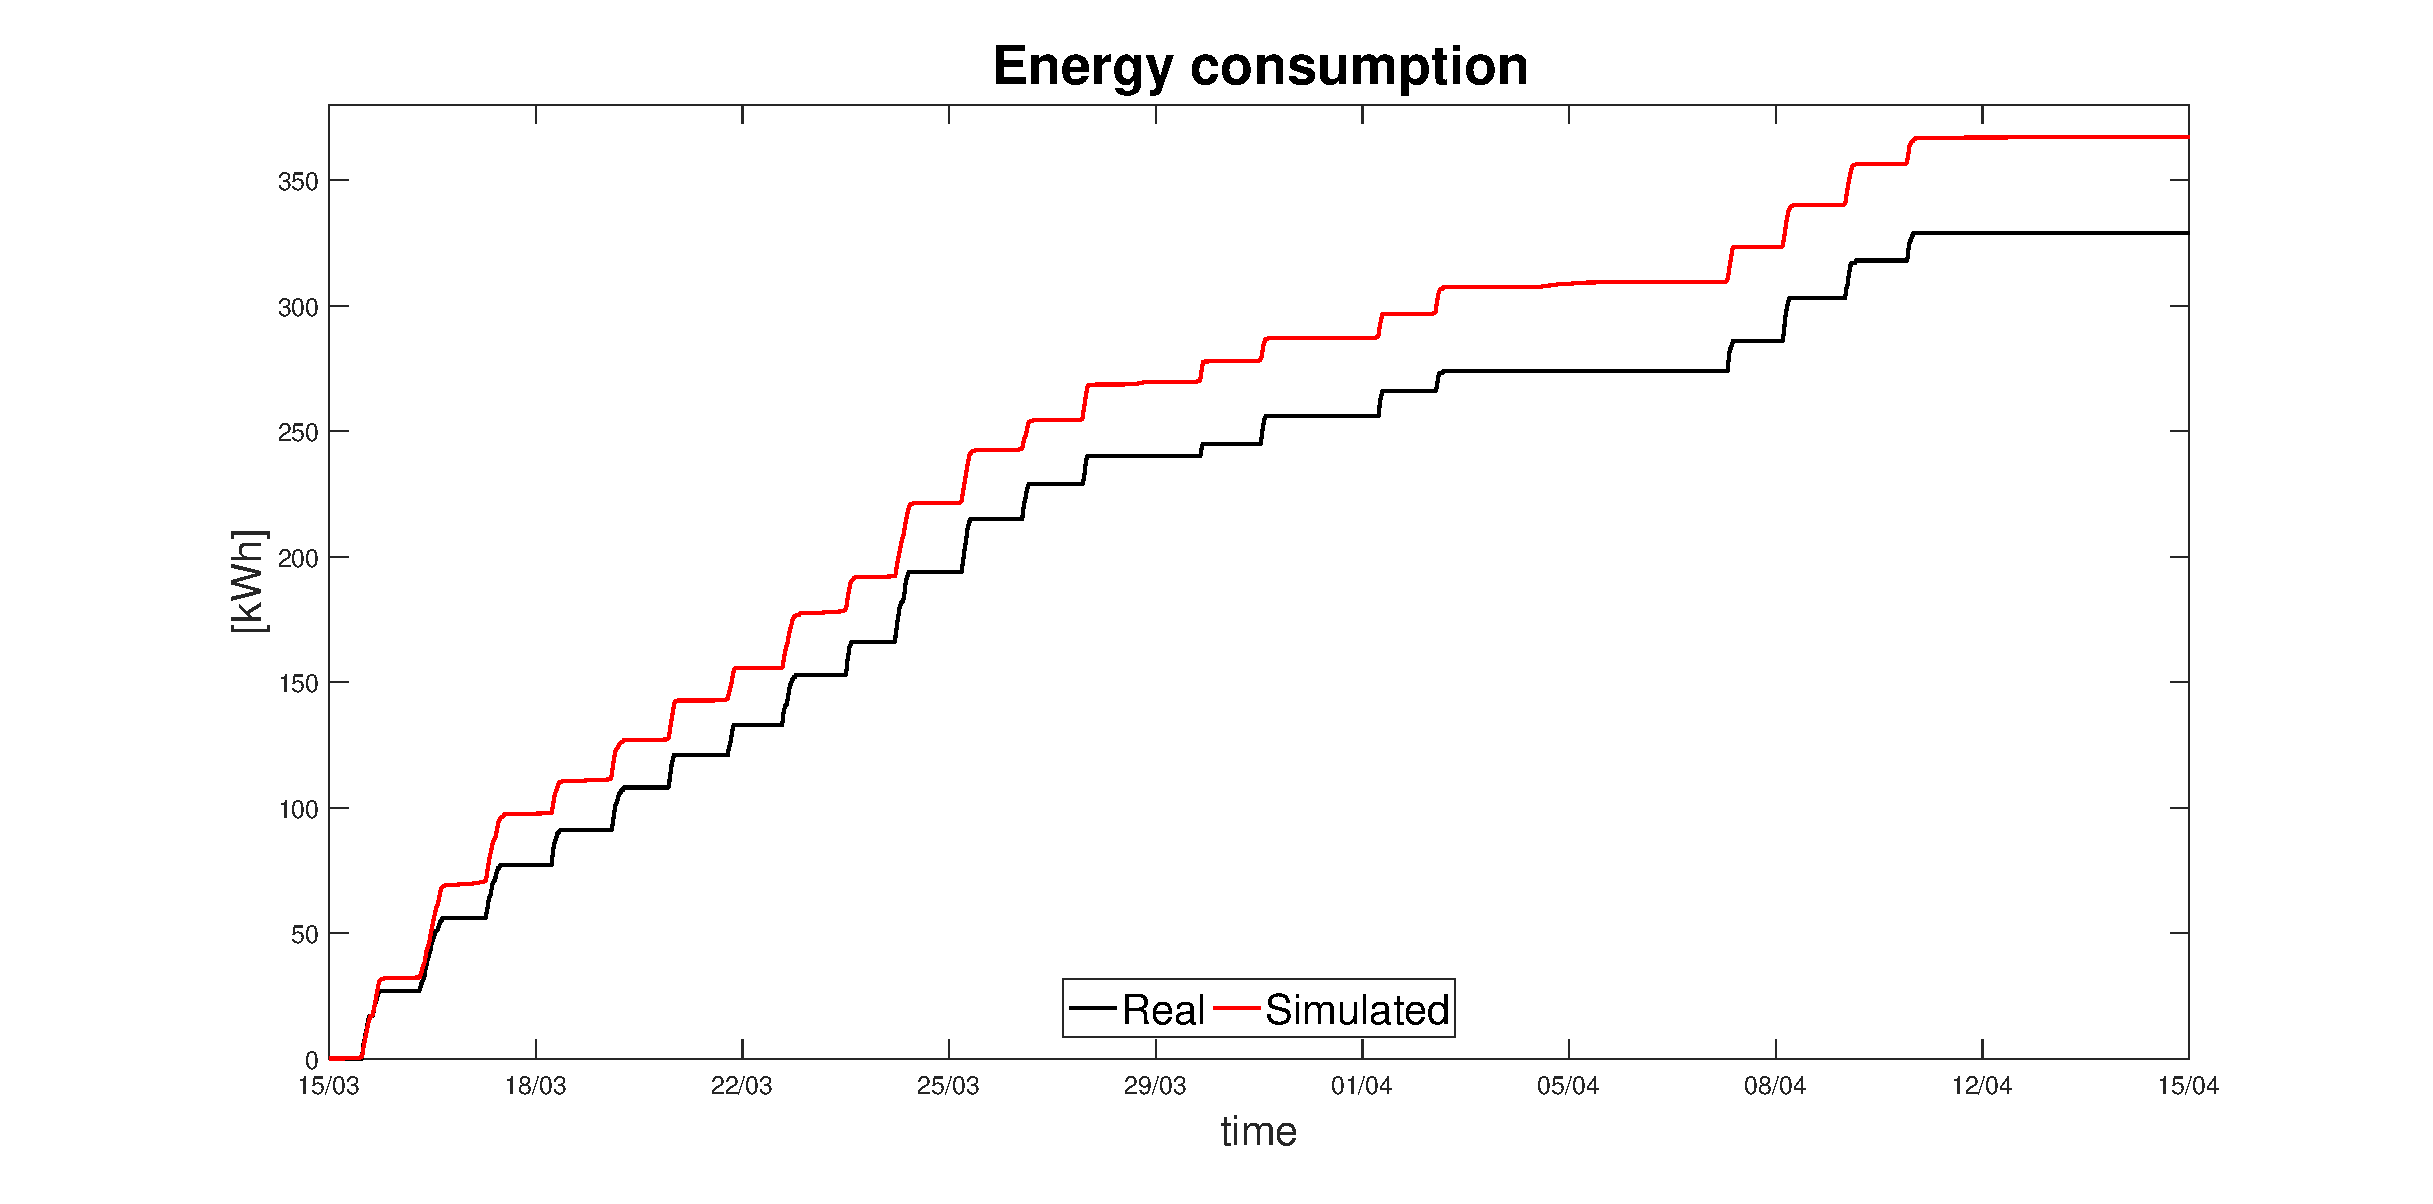
\includegraphics[width=26pc]{figures/Energy_test.eps}
%		\caption{Energy consumption accuracy.}
%		\captionsetup{justification=centering}
%		\label{F:Energy_testing}
%	\end{center}
%\end{figure}
%
%As we can see, with random forest model we get a worse MBE and CV(RMSE) for energy consumption, although the maximum error is very similar. This is because the EnergyPlus model, due to its internal dynamics based on the house structure, is able to compensate the error over time. On the other hand our curve perfectly follows the time behavior of the real case. For this reason, in Section \ref{SS:simulationResults}, we will use both models in order to compare the quality of the DPC with respect to a classical bang-bang controller.

\subsection{DPC and bang-bang controllers}
\label{SS:controllersDPCandBangbang}
We set up $2$ different controllers, DPC and bang-bang controller, to obtain a scheduling policy to switch the radiators ON and OFF in order to keep the temperature of room $3$, i.e. the living room, within a comfort range. Since the heating system serves all of the $4$ rooms simultaneously, without giving the possibility to control the temperature of each room independently, we setup the problem defining the comfort range only for one room. Other rooms temperatures will follow the scheduling policy. Room $3$ has been chosen randomly. In the following we describe the $2$ controllers.

\paragraph{DPC}
We want to optimize the ON/OFF heating system schedule in order to minimize power consumption of the house while keeping temperature of room $3$ within a comfort range. We also allow violations $\epsilon^{min},\epsilon^{max}$  of temperature bounds to guarantee feasibility of the algorithm. We include these violations in the objective function to be minimized.
\begin{table}[t!]
	\centering
	\begin{tabular}{cccccc}
		\toprule
		Set       & Power   & T. room $1$ & T. room $2$ & T. room $3$ & T. room $4$  \\ 
		\midrule
		$S_1$     &         & $96.58$     & $96.99$     & $97.21$     & $96.62$\\
		$S_2$     & $92.21$ & $97.38$     & $97.29$     & $96.93$     & $96.81$\\
		\bottomrule
	\end{tabular}
	\caption{Models accuracy for power and temperatures models in $S_1$ and $S_2$ expressed as $\mathrm{1-NRMSE}\,(\%)$.}
	\captionsetup{justification=centering}
	\label{T:S1accuracy}
	\vspace{-0.5cm}
\end{table}

The problem is set up as follows:

\begin{problem}\label{P:dpcRealCase}
	\begin{align}
		\begin{aligned}
		& \underset{u_{k+j-1},\epsilon_j^{min},\epsilon_j^{max}}{\mathrm{minimize}} & & \sum_{j=1}^{N} Q{\tP}_{k+j}^2 + \lambda_{min}\parallel\epsilon^{min}\parallel_2 + \lambda_{max}\parallel\epsilon^{max}\parallel_2                            \\
		& \mathrm{subject\ to } & & \tP_{k+j}   = \hat{\Theta}_{\tP_j}   [ 1,u_k,\ldots,u_{k+j-1} ]^\top                         \\
		&                    & & \tT^1_{k+j} = \hat{\Theta}_{\tT^1_j} [ 1,u_k,\ldots,u_{k+j-1} ]^\top                            \\
		&                    & & \tT^2_{k+j} = \hat{\Theta}_{\tT^2_j} [ 1,u_k,\ldots,u_{k+j-1} ]^\top                            \\
		&                    & & \tT^3_{k+j} = \hat{\Theta}_{\tT^3_j} [ 1,u_k,\ldots,u_{k+j-1} ]^\top                            \\
		&                    & & \tT^4_{k+j} = \hat{\Theta}_{\tT^4_j} [ 1,u_k,\ldots,u_{k+j-1} ]^\top                            \\
		&                    & & \underline{\tT}_{k+j}-\epsilon^{min}_j\leq\tT^3_{k+j}\leq\overline{\tT}_{k+j}+\epsilon^{max}_j  \\
		&                    & & u_{k+j-1}   = \underline{u} \lor u_{k+j-1} = \overline{u}                                       \\
		&                    & & \epsilon^{min}_j,\epsilon^{max}_j \geq 0, \ j = 1,\dots,N.
		\end{aligned}
	\end{align}\label{E:DPCrealcase}
\end{problem}

\begin{figure}[t!]
	\begin{center}
		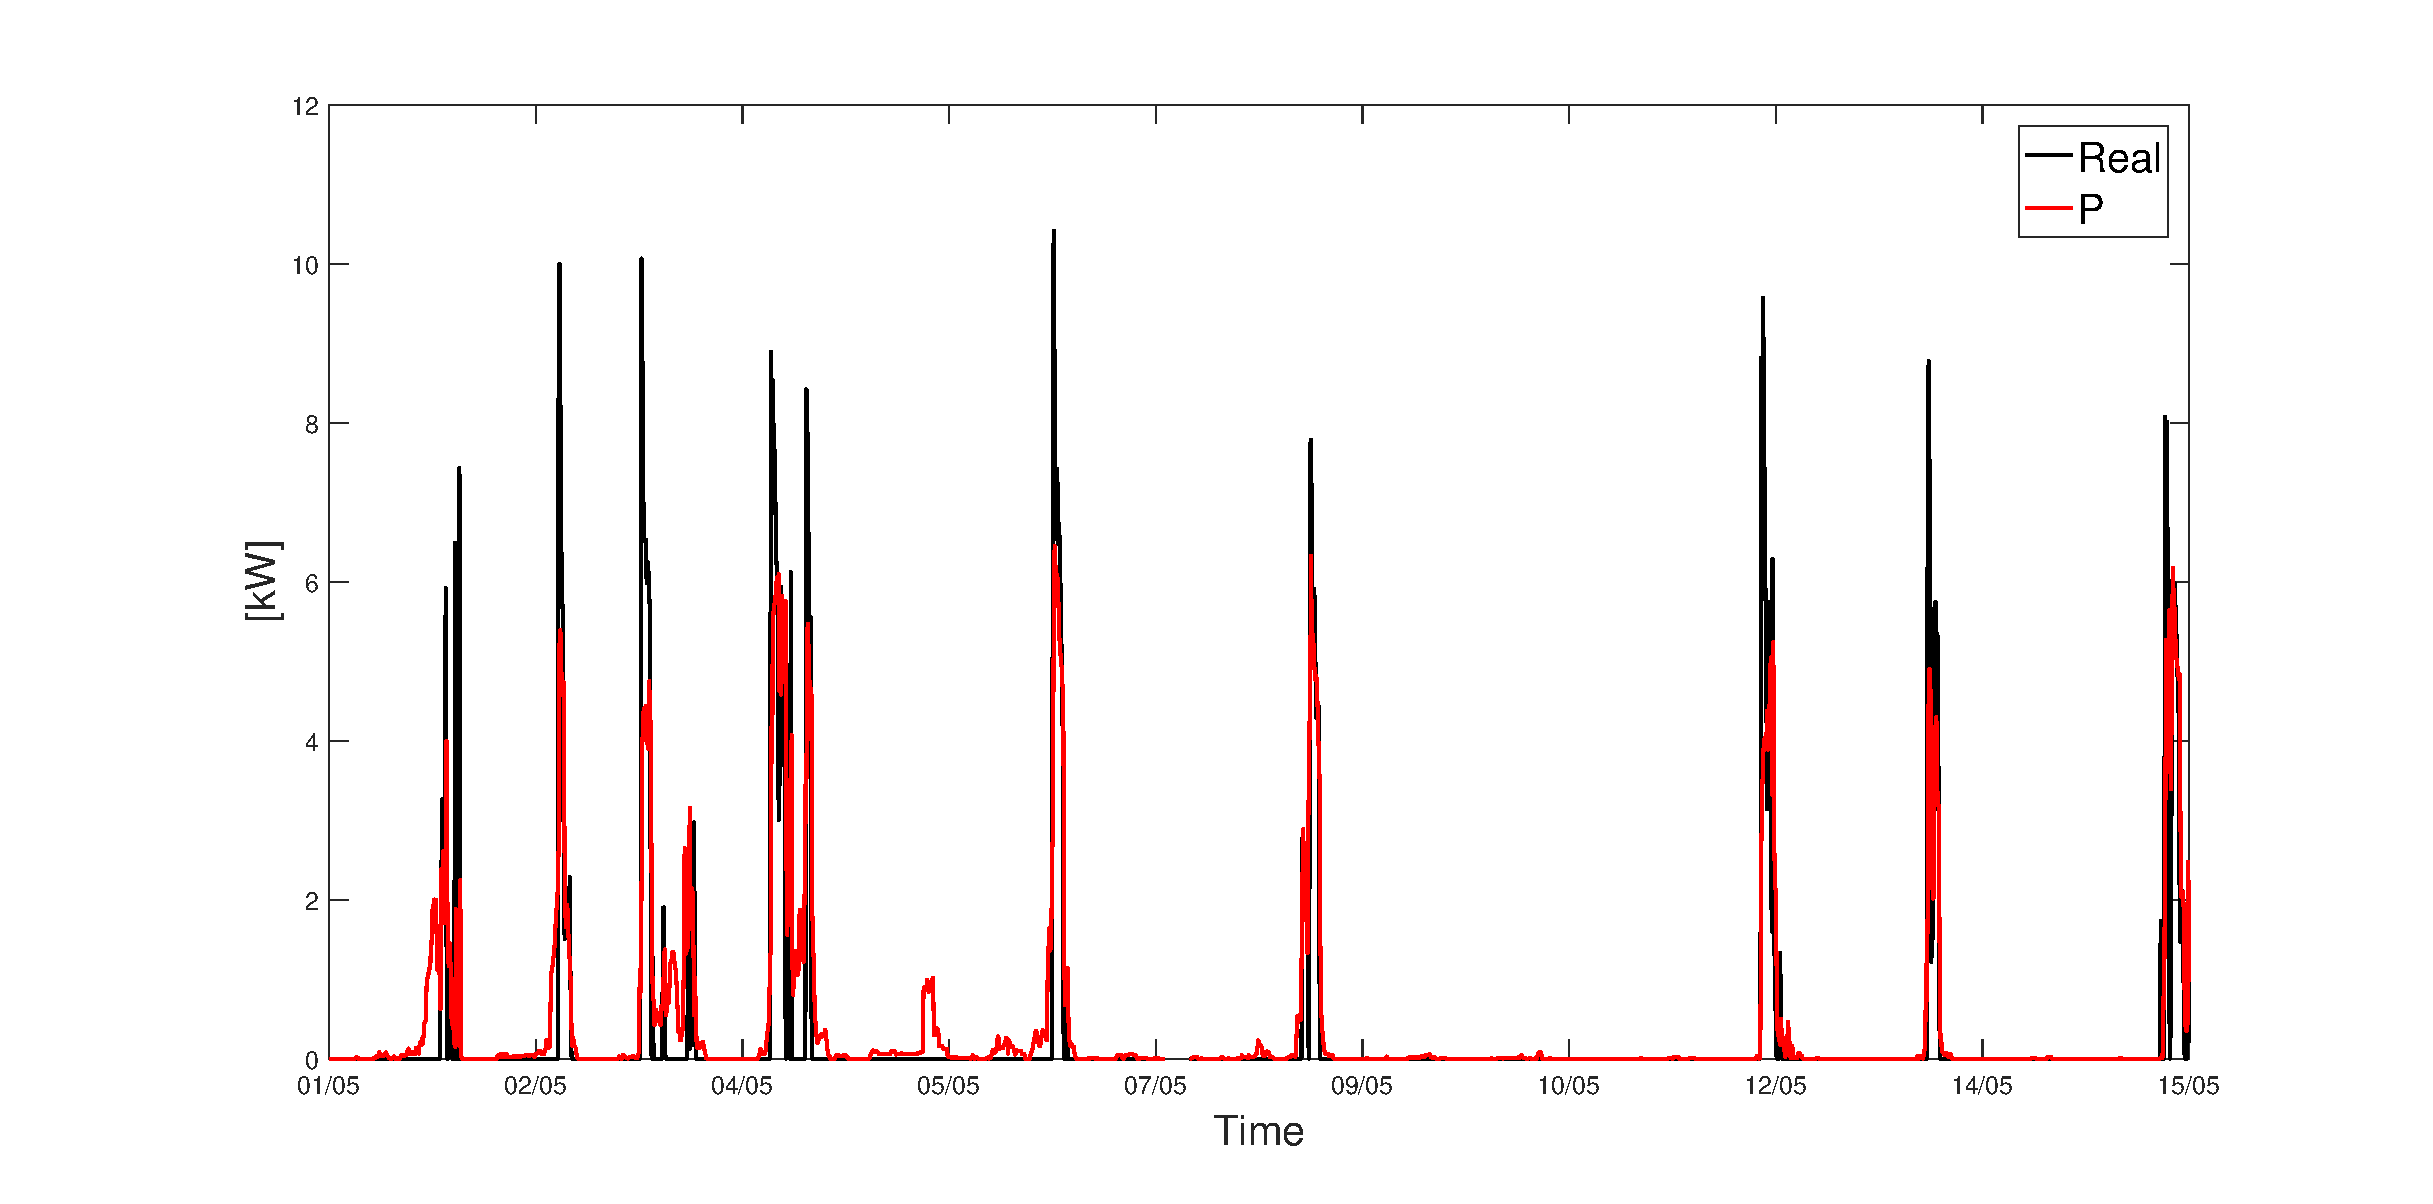
\includegraphics[width=26pc]{figures/power_testing.eps}
		\caption{Power consumption model accuracy validation. The accuracy over the testing period expressed as $\mathrm{1-NRMSE}\,(\%)$ is $92.1\%$.}
		\label{F:power_testing}			
	\end{center}
\end{figure}

\begin{figure}[t!]
	\begin{center}
		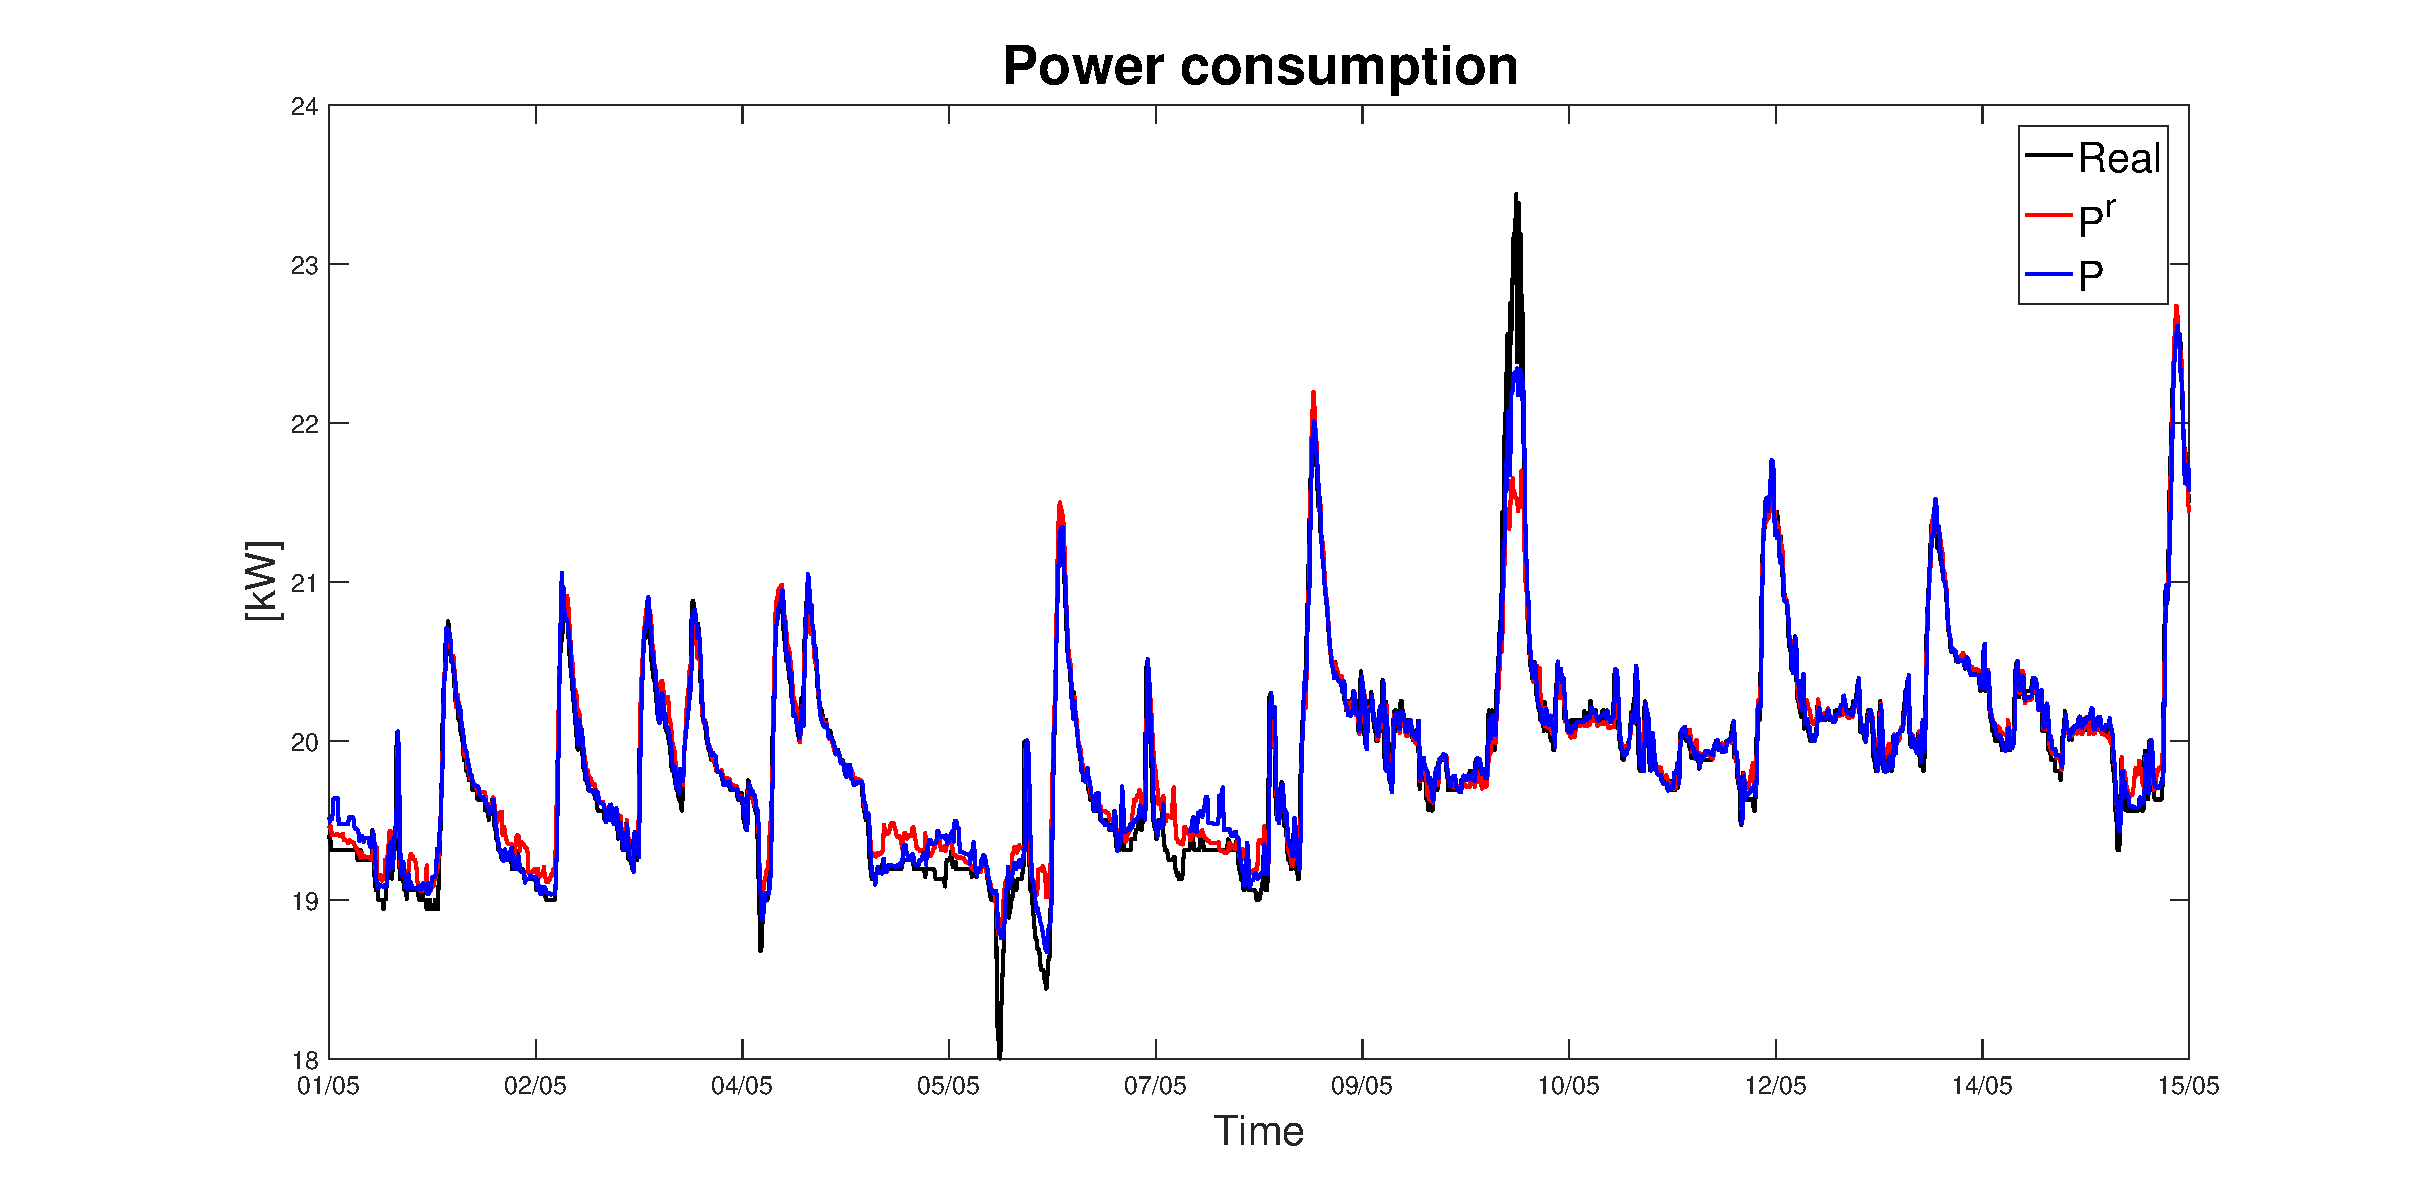
\includegraphics[width=26pc]{figures/temperature_testing.eps}
		\caption{Temperature model accuracy validation for room $1$. The accuracy over the testing period expressed as $\mathrm{1-NRMSE}\,(\%)$ is $96.58\%$, for the temperature model $T^{r_1}$ in $S_1$ and $97.3\%$ for the temperature model $T^1$ in $S_2$. The accuracy for the other rooms is very similar as can be seen in Table \ref{T:S1accuracy}.}
		\label{F:temperature_testing}	
	\end{center}
\end{figure}

The choice of different weights $Q$, $\lambda_{min}$ and $\lambda_{max}$ allows the designer to give more importance to energy consumption rather than temperature comfort and vice versa.
In Section \ref{SS:simulationResults} we will show different performance results considering different weights. Parameters $\underline{u}$ and $\overline{u}$ are respectively minimum and maximum values the heating system can actuate, while $\underline{\tT}_{k+j-1}$ and $\overline{\tT}_{k+j-1}$ are respectively time varying lower and upper bounds to keep the temperature in a desired range of comfort.
Due to the integer variable constraint for input $u$, the problem is a Mixed Integer Quadratic Programming. For the implementation we use in Section \ref{SS:simulationResults} Gurobi solver \cite{Gurobi2015} through CVX \cite{cvx,gb08}.

\paragraph{Bang-bang controller}
This is the classical controller widely used in private houses to keep temperature within a comfort range. It switches the heating system ON when the temperature goes under the temperature lower bound and switches it OFF when the temperature goes over the temperature upper bound. The advantage in using this controller is that it is very simple to set up. On the other hand it uses more energy than actually needed to achieve the task.

\subsection{Simulation Results}\label{SS:simulationResults} We simulated  DPC in \eqref{E:DPCrealcase} and the bang-bang controller, in closed-loop with the house models $\tT^{r_i}_{k+1},\ i=1,\ldots,4$ in $S_1$. We considered a sampling time of $10$ minutes and chose $N=4$ as a predictive horizon, i.e. $40$ minutes. From historical data we got that $\overline{u} = 0.35 \, m^3/h$ when the heating system is ON and obviously $\underline{u} = 0 \, m^3/h$ when the heating system is OFF. For the temperature comfort range we set a constant upper bound $\overline{\tT}_{k} = 22.5 \, \degree C$ and a variable lower bound that is $\underline{\tT}_{k} = 21 \, \degree C$ from $7am$ to $9am$ when people in the house wake up and go out for work, and from $6pm$ to midnight when people come back from work and go to sleep. During other hours when people are either not at home or asleep, we set $\underline{\tT}_{k} = 20 \, \degree C$ 

We explained in Section \ref{SS:descriptionHouse} that the fuel used in the house is vegetable biomass. Therefore, it is not possible to have ON/OFF switching phases too close to each other, differently from a traditional gas boiler, due to the burning process and heat exchange. For this reason we set up both control problems with the constraint that when the heating system is activated it must stay active for at least $20$ minutes. This operating period can be obviously adapted depending on the fuel flow rate.

We ran DPC with $3$ different sets of parameters $Q$, $\lambda_{min}$ and $\lambda_{max}$. Each set allows a different level of temperature bounds violation. In particular, we considered a small ($Q=100$, $\lambda_{min}=3000$ and $\lambda_{max}=100$), a medium ($Q=100$, $\lambda_{min}=1000$ and $\lambda_{max}=100$) and a large ($Q=100$, $\lambda_{min}=100$ and $\lambda_{max}=100$) violation configuration.
\textcolor[rgb]{0,0,1}{The simulation period is of $15$ days, from May $1$, $2016$ at $00am$ to May $15$, $2016$ $00am$.}

\textcolor[rgb]{0,0,1}{We considered 2 different simulative conditions to show the robustness of our approach:
\begin{enumerate}
	\item in Section \ref{SSS:DisturbancePerfect} we provide our simulative results considering perfect knowledge of the weather forecast;
	\item in Section \ref{SSS:DisturbanceUncertain}, we consider weather forecast subject to uncertainty Hence we modify Problem \ref{P:dpcRealCase} by adding a gaussian noise with high variance on the perfect forecast, and show that the results are close to the perfect forecast case, so making our methodology robust with respect to disturbance uncertainties.
\end{enumerate}
\subsubsection{Perfect knowledge of the weather forecast}\label{SSS:DisturbancePerfect}
In this section we ran the simulations considering perfect knowledge of the disturbance over the horizon, obtaining the following results.}
\paragraph{Result 1} The comparison for temperature and input schedule obtained allowing small bound violations in DPC is shown in Figure \ref{F:comparison_small}. For sake of the plot's clarity, the shown period is restricted to $4$ days and a half, from May $1$, $2016$ $00am$ to May $5$, $2016$ $1pm$. \textcolor[rgb]{0,0,1}{The whole period will be used in "Result 2" to provide the bounds violation errors, and in "Result 3" for the energy consumption comparison.}
We can see that the temperature controlled with DPC does not violate the bounds and if it does then the violation is approximately $0.1\,\degree C$. Bang-bang control also presents small bounds violations due to its working principle. We can see how the DPC control law requires the heating system to be ON for less time than the bang-bang one to keep the temperature in the comfort range. 
We will see in Figure \ref{F:comparison_all_energy_E+} that this translates to significant energy saving.

\begin{figure}[t!]
	\begin{center}
	\subfigure[Temperature variation obtained with DPC and bang-bang controller.DPC controller allows almost no violation, so guaranteeing better comfort than bang-bang controller.]{
		\label{F:temperatures_small}
		\centering
		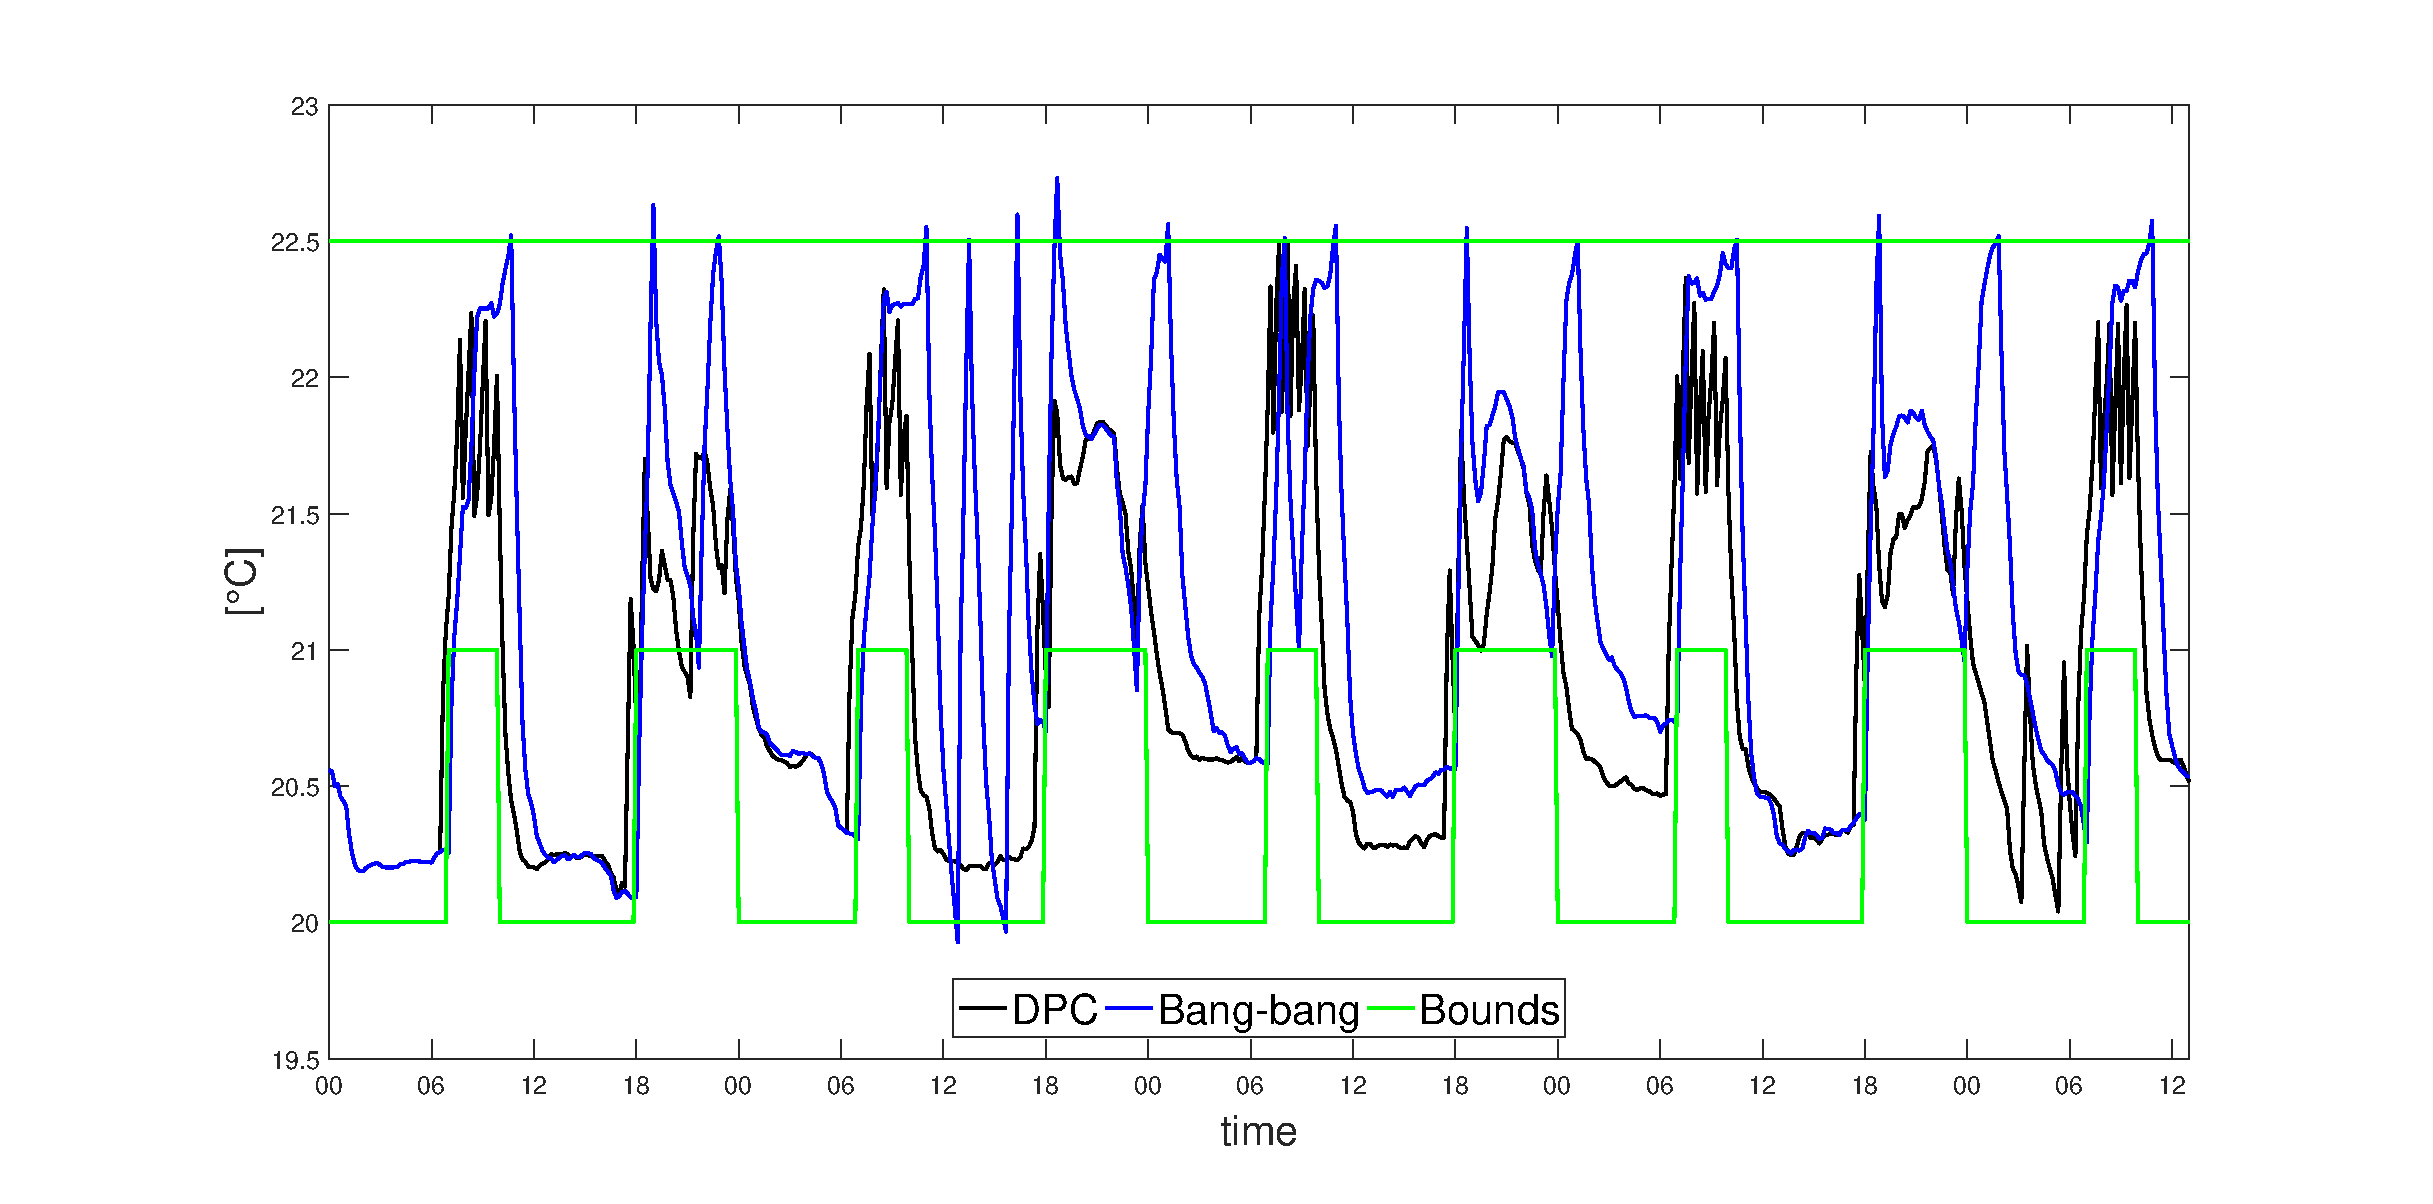
\includegraphics[width=28pc]{figures/Temperatures_small.eps}
	}
	\subfigure[Input schedules obtained from DPC and bang-bang controller. DPC keeps the heating system ON for less time than bang-bang controller, hence saving energy, and guarantees better thermal comfort.]{
		\label{F:inputs_small}
		\centering
		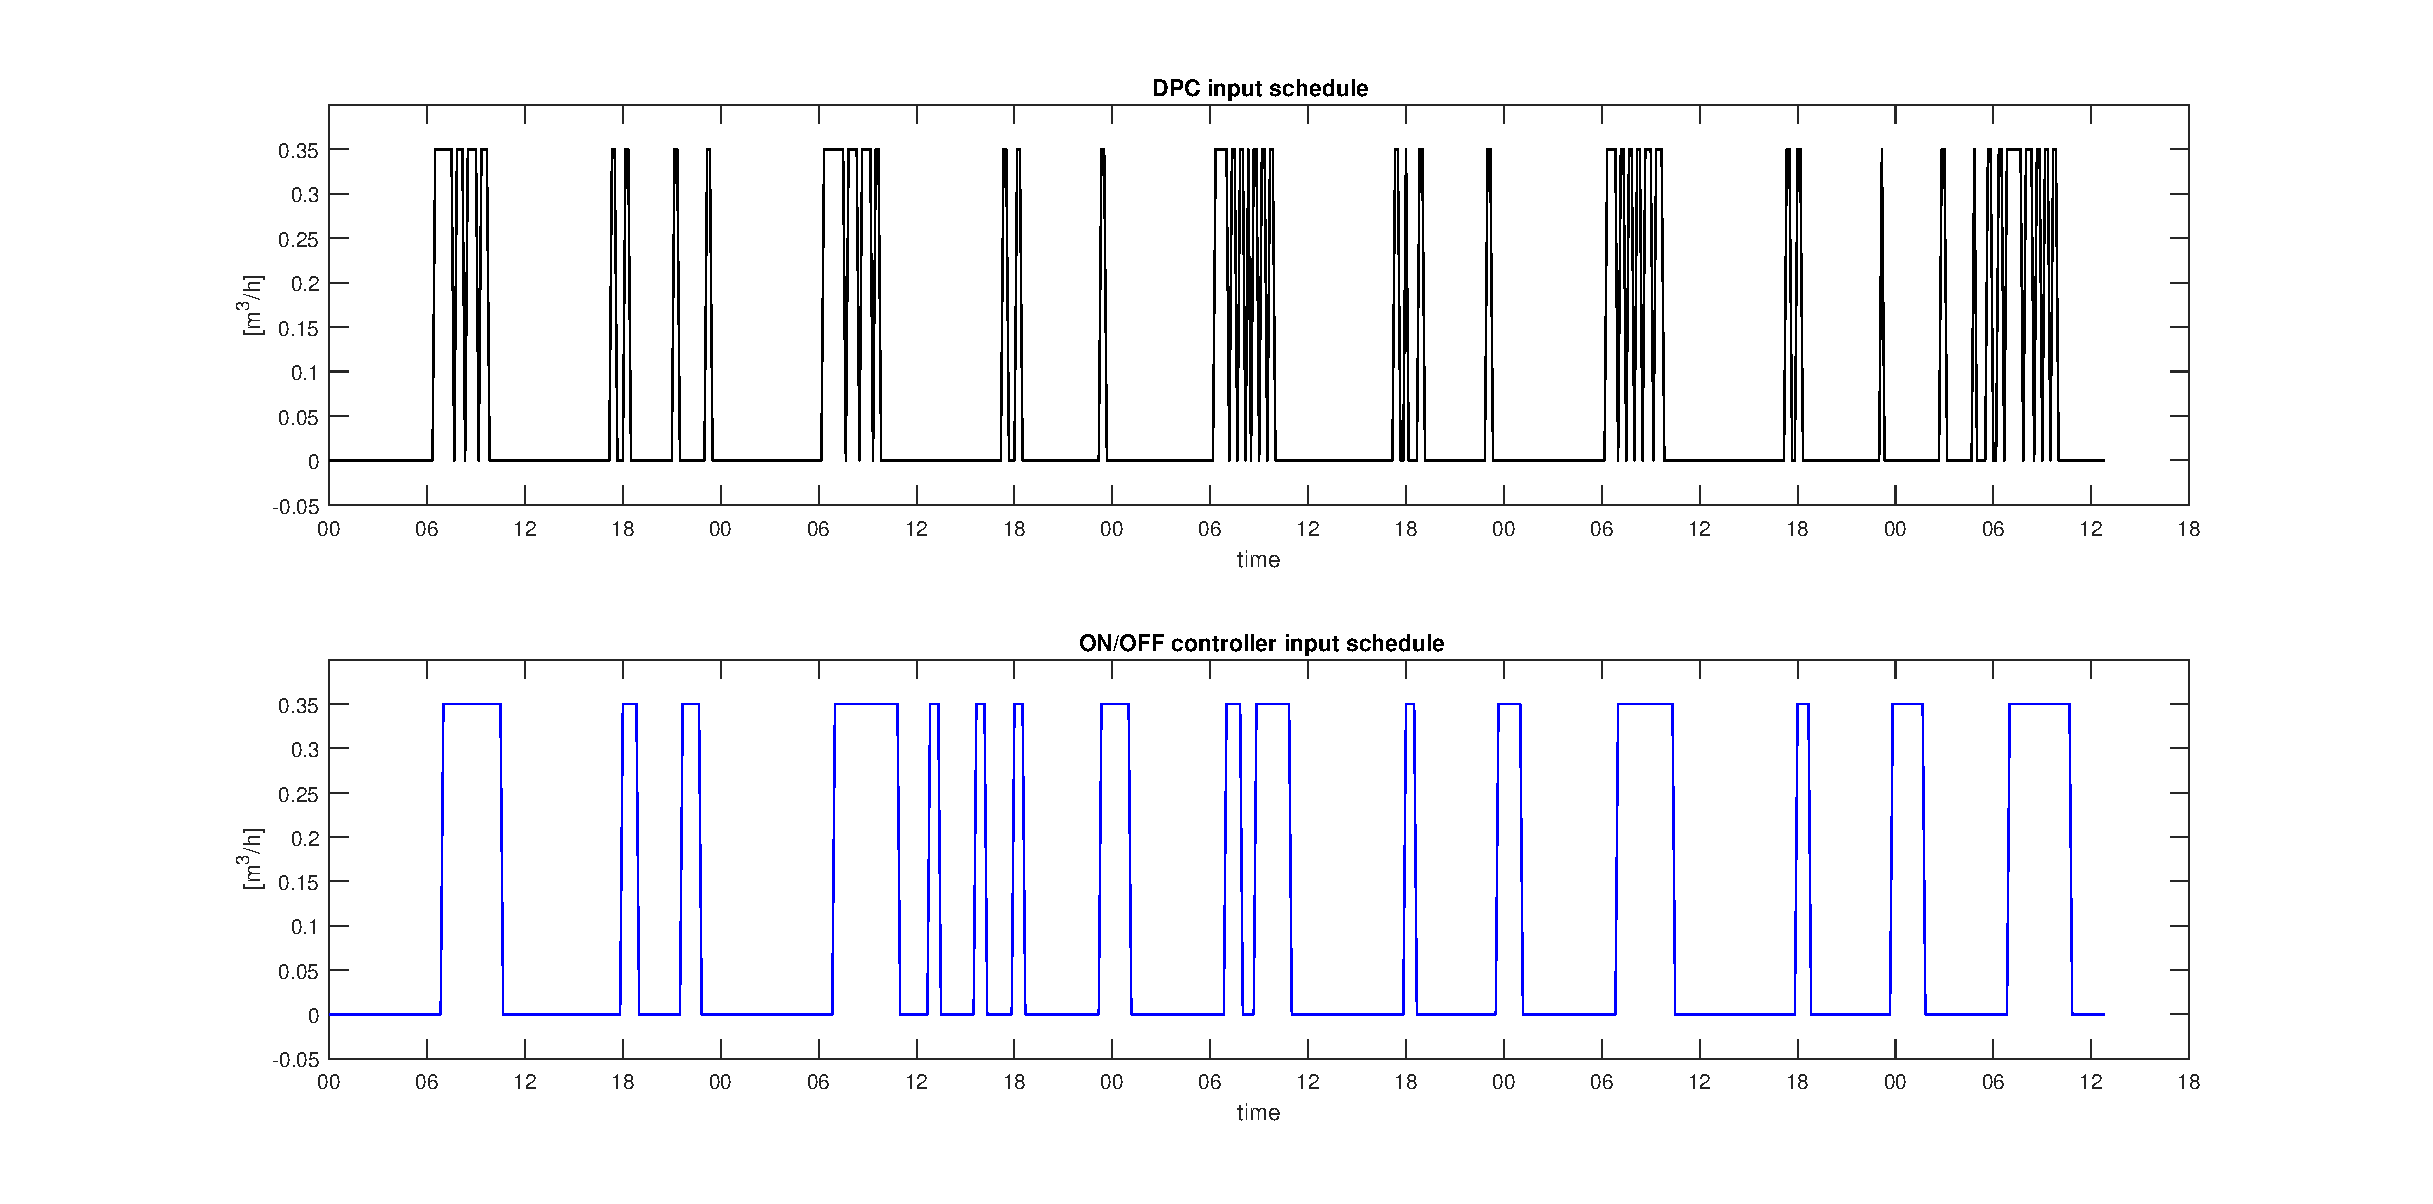
\includegraphics[width=28pc]{figures/Inputs_small.eps}
	}
	\end{center}
\vspace{-0.5cm}
	\caption{Comparison of DPC and bang-bang control performance over $5$ days of the testing period for room $3$.}
	\captionsetup{justification=centering}
	\label{F:comparison_small}
\end{figure}

\paragraph{Result 2} A comparison of temperature regulation obtained running the DPC with small, medium and large violations is shown in Figure \ref{F:comparison_all_temperature}. The results show that with the large violation configuration, that gives more importance to the power consumption minimization than to keep temperature within the bounds, temperature is almost always outside the lower bound during the period when the range is tighter. However the maximum violation is still lower than $1\,\degree C$.
In Table \ref{T:violationErrors}, MBE and CV(RMSE)\textcolor[rgb]{0,0,1}{ (expressed in $\%$, and computed over the whole simulative period, i.e. 15 days) }violation errors are reported to quantify the bounds violation of DPC, in each of the $3$ configurations, and of bang-bang controller. We can see that if we allow very small violations, DPC outperforms bang-bang controller in terms of comfort guarantees.

\paragraph{Result 3} 
%In Figure \ref{F:comparison_all_energy_E+}, using the energy model derived from random forest power model $\tP^r$, we show how DPC outperforms the bang-bang controller also in terms of energy consumption and how the bounds violations allow us to save more energy. We can see that if we want to keep the temperature within a comfort range, only allowing small violations, the use of DPC produce an energy saving of $44\, kWh$, that correspond to the $33.0\%$ over a period of $4$ days and a half. Instead if we allow a large violation over the same period, the energy saving is of $78\, kWh$, that correspond to the $59.0\%$. If we consider these results over a monthly period, i.e. multiplying them for $6$, we get a monthly energy saving that goes from $264\,kWh$ to $468\,kWh$, with different comfort constraint configurations. Considering that the equivalent price of $1\,kWh$ of vegetable biomass is $TOT$\euro{} (TULLIO MAY YOU TELL ME ABOUT THIS PART?), we have a monthly saving of $TOT$\euro{}.

%\begin{figure}[h!]
%	\begin{center}
%		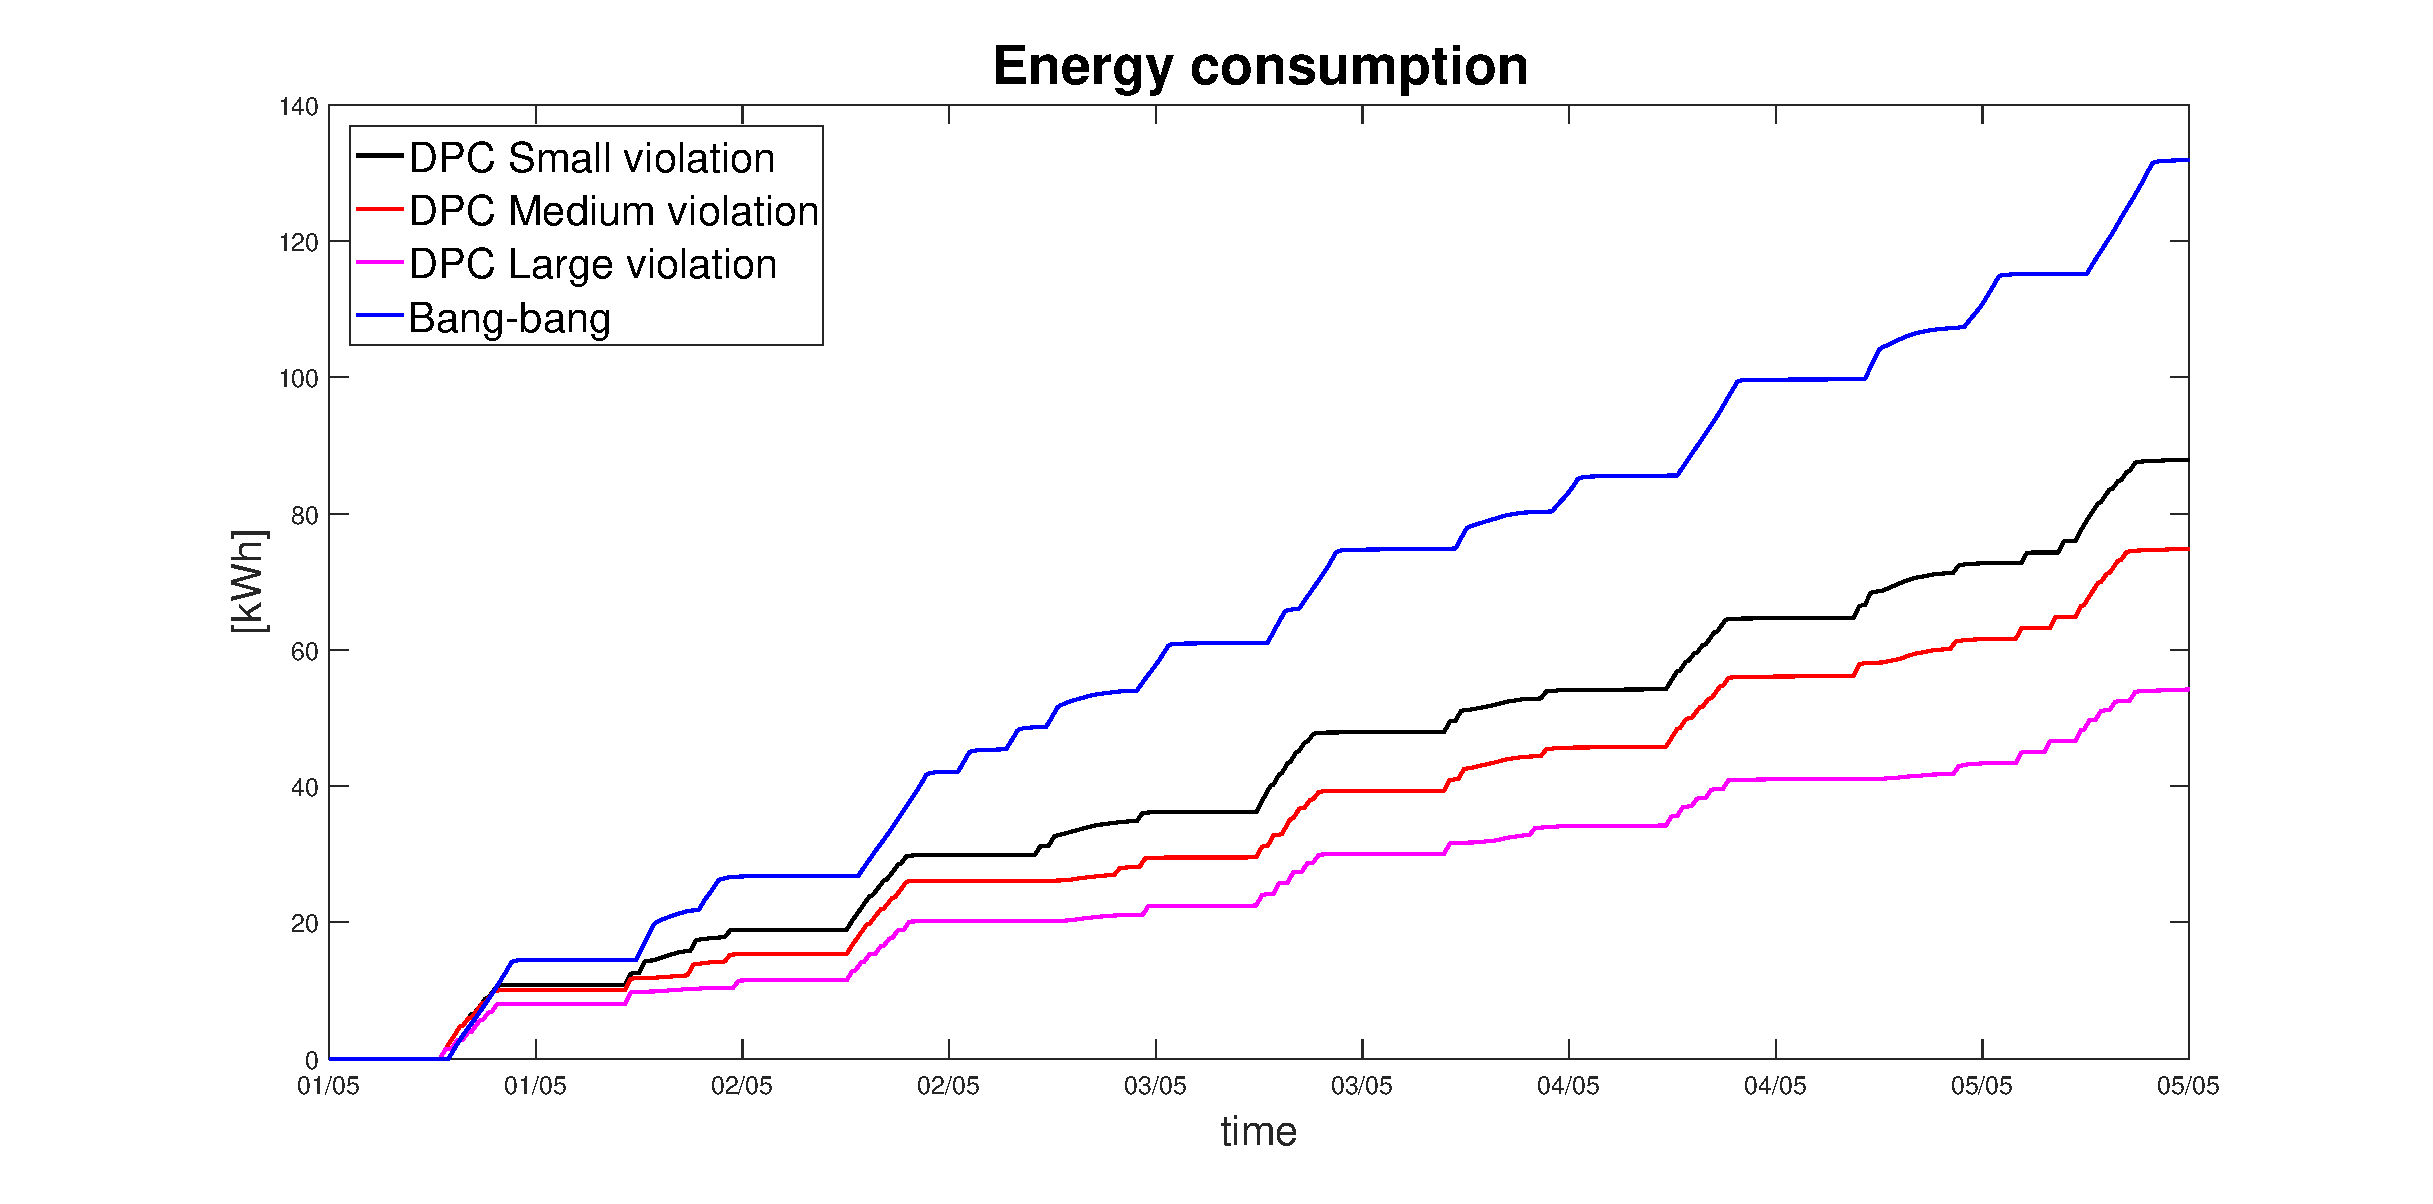
\includegraphics[width=26pc]{figures/Energy_all.eps}
%	\end{center}
%	\caption{Comparison of DPC and bang-bang control performance with different violations using random forest model.}
%	\label{F:comparison_all_energy}
%\end{figure}
%An alternative comparison can be done considering the EnergyPlus model of the house for energy consumption described in Section \ref{SS:energyPlusmodel}. Results are shown in Figure \ref{F:comparison_all_energy_E+}.
In Figure \ref{F:comparison_all_energy_E+}, using the thermal energy consumption model derived in Section \ref{SS:energyPlusmodel} using EnergyPlus, we show how DPC outperforms the bang-bang controller also in terms of energy consumption and how the bounds violations allow us to save more energy. In this case, since the plot is clear and we are interested in showing energy saving on a long period, we ran the simulations over the whole testing period, i.e. $15$ days of May, from May $1$, $2016$ to May $15$, $2016$. We observe that the energy consumption associated to the bang-bang control strategy is approximately equal to $177\,kWh$. If we want to keep the temperature within a comfort range, only allowing small violations, the use of DPC produce an energy saving of $45\, kWh$, that corresponds to the $25.4\%$ over a period of $15$ days. In case of medium violations get an energy saving of $57\, kWh$, that is $32.2\%$. Instead if we allow a large violation over the same period, the energy saving is of $87\, kWh$, that corresponds to the $49.2\%$.
\begin{figure}[t!]
	\begin{center}
		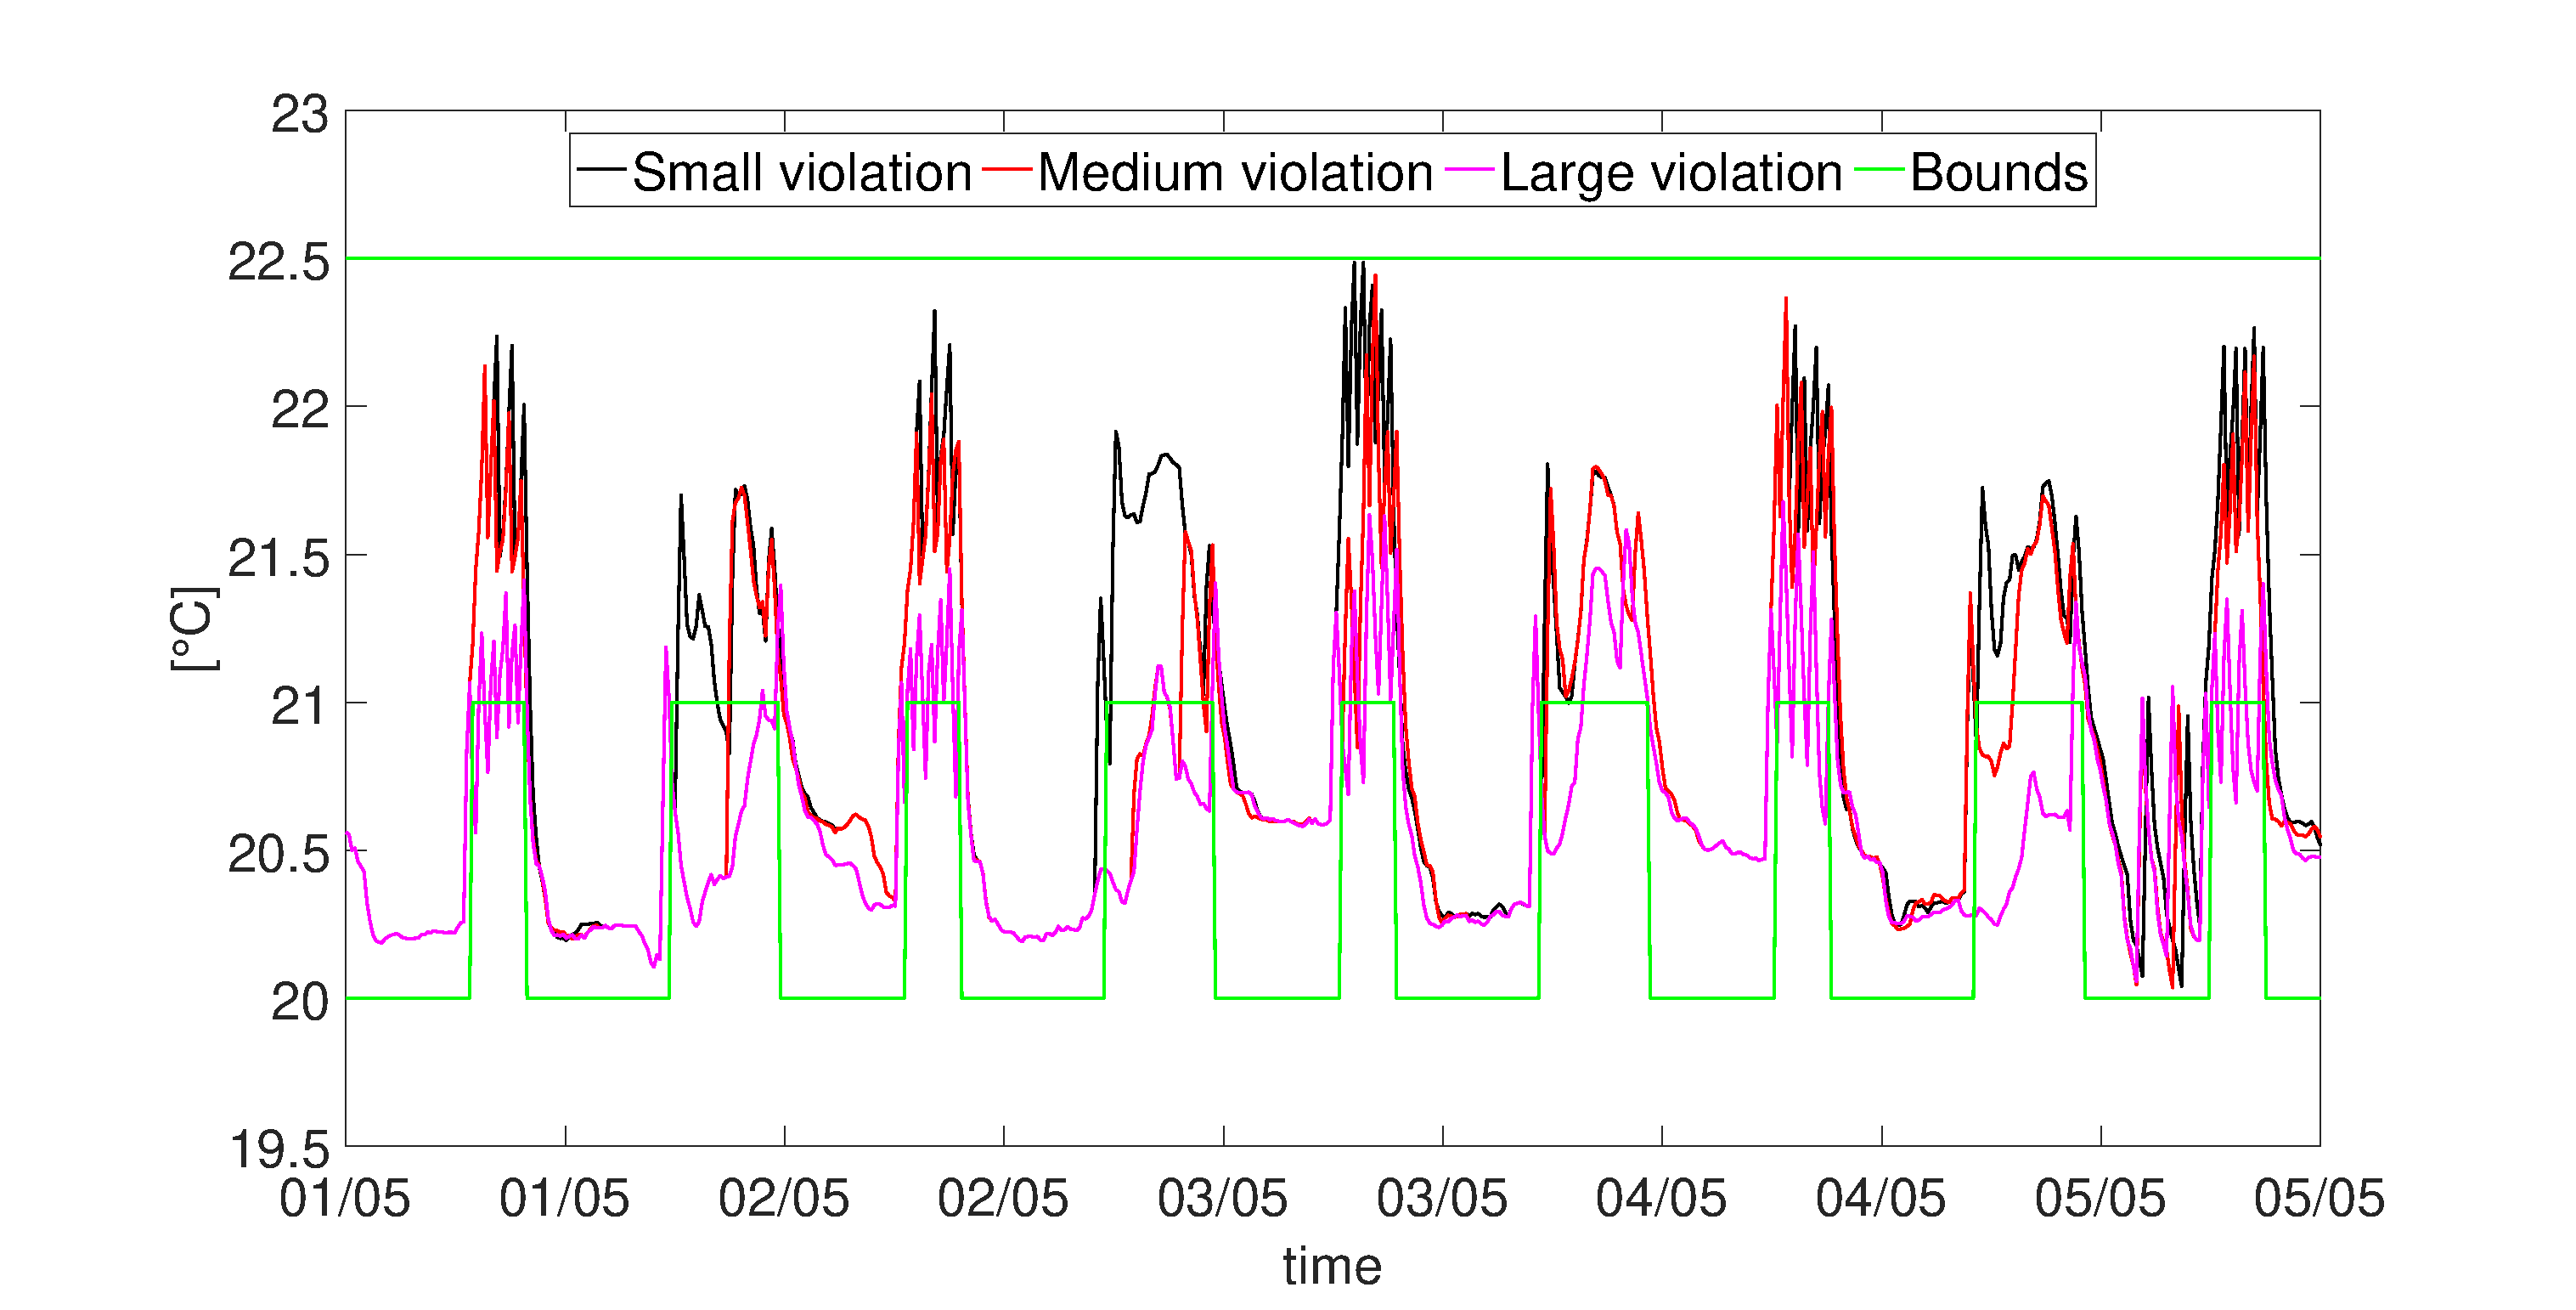
\includegraphics[width=28pc]{figures/Temperatures_all.eps}
	\end{center}
	\caption{Comparison, in terms of comfort, of DPC control performance simulated over $5$ days of the testing period with $3$ different violation configurations: small, medium and large. With the large violation configuration, the temperature is almost always outside of the lower bound when this is tighter. However the maximum bound violation is less than $1\degree C$. With the small violation configuration, the temperature is always within the bound with very few exceptions. However, when it happens, the violation is lower than $0.1\degree C$. The medium violation configuration gives a temperature bound violation that is in the middle with respect to the small and the large ones.}
	\label{F:comparison_all_temperature}
\end{figure}
%\begin{table}[t!]
%	\centering
%	%	\scalebox{0.9}{
%	\begin{tabular}{lccccc}
%		\toprule
%		CONTROLLER  & LBV $\mathrm{MBE}$  & LBV $\mathrm{RMSE}$ & UBV $\mathrm{MBE}$ & UBV $\mathrm{RMSE}$ 	\\ 
%		\midrule
%		$DPC-SV$    & $0.013$             & $0.028$  			      & $0$    				 & $0$     	  	\\
%		$DPC-MV$    & $0.165$ 			  & $0.146$     			  & $0$    				 & $0$		  	\\
%		$DPC-LV$    & $0.410$  			  & $0.224$     			  & $0$    				 & $0$	      	\\
%		$Bang-bang$ & $0.049$ 			  & $0.080$    				  & $0.0063$ 		     & $0.0120$	  	\\
%		\bottomrule
%	\end{tabular}
%	%	}
%	\caption{Lower Bound Violation (LBV) and Upper Bound Violation (UBV) errors expressed as $\mathrm{MBE}\%$ and $\mathrm{CV(RMSE)}\%$ for DPC Small Violation (DPC-SV), DPC Medium Violation (DPC-MV), DPC large Violation (DPC-LV) and bang-bang controller.}
%	\captionsetup{justification=centering}
%	\label{T:violationErrors}
%\end{table}
\begin{table}[t!]
	\centering
	%	\scalebox{0.9}{
	\begin{tabular}{lccccc}
		\toprule
		CONTROLLER  & LBV $\mathrm{MBE}$  & LBV $\mathrm{RMSE}$ & UBV $\mathrm{MBE}$ & UBV $\mathrm{RMSE}$ 	\\ 
		\midrule
		$DPC-SV$    & $0.013$             & $0.092$  			      & $0$    				 & $0$     	  	\\
		$DPC-MV$    & $0.165$ 			  & $0.479$     			  & $0$    				 & $0$		  	\\
		$DPC-LV$    & $0.410$  			  & $0.733$     			  & $0$    				 & $0$	      	\\
		$Bang-bang$ & $0.0485$ 			  & $0.265$    				  & $0.0063$ 		     & $0.040$	  	\\
		\bottomrule
	\end{tabular}
	%	}
	\caption{Lower Bound Violation (LBV) and Upper Bound Violation (UBV) errors expressed as $\mathrm{MBE}\%$ and $\mathrm{CV(RMSE)}\%$ for DPC Small Violation (DPC-SV), DPC Medium Violation (DPC-MV), DPC large Violation (DPC-LV) and bang-bang controller.}
	\captionsetup{justification=centering}
	\label{T:violationErrors}
\end{table}
\begin{figure}[t!]
	\begin{center}
		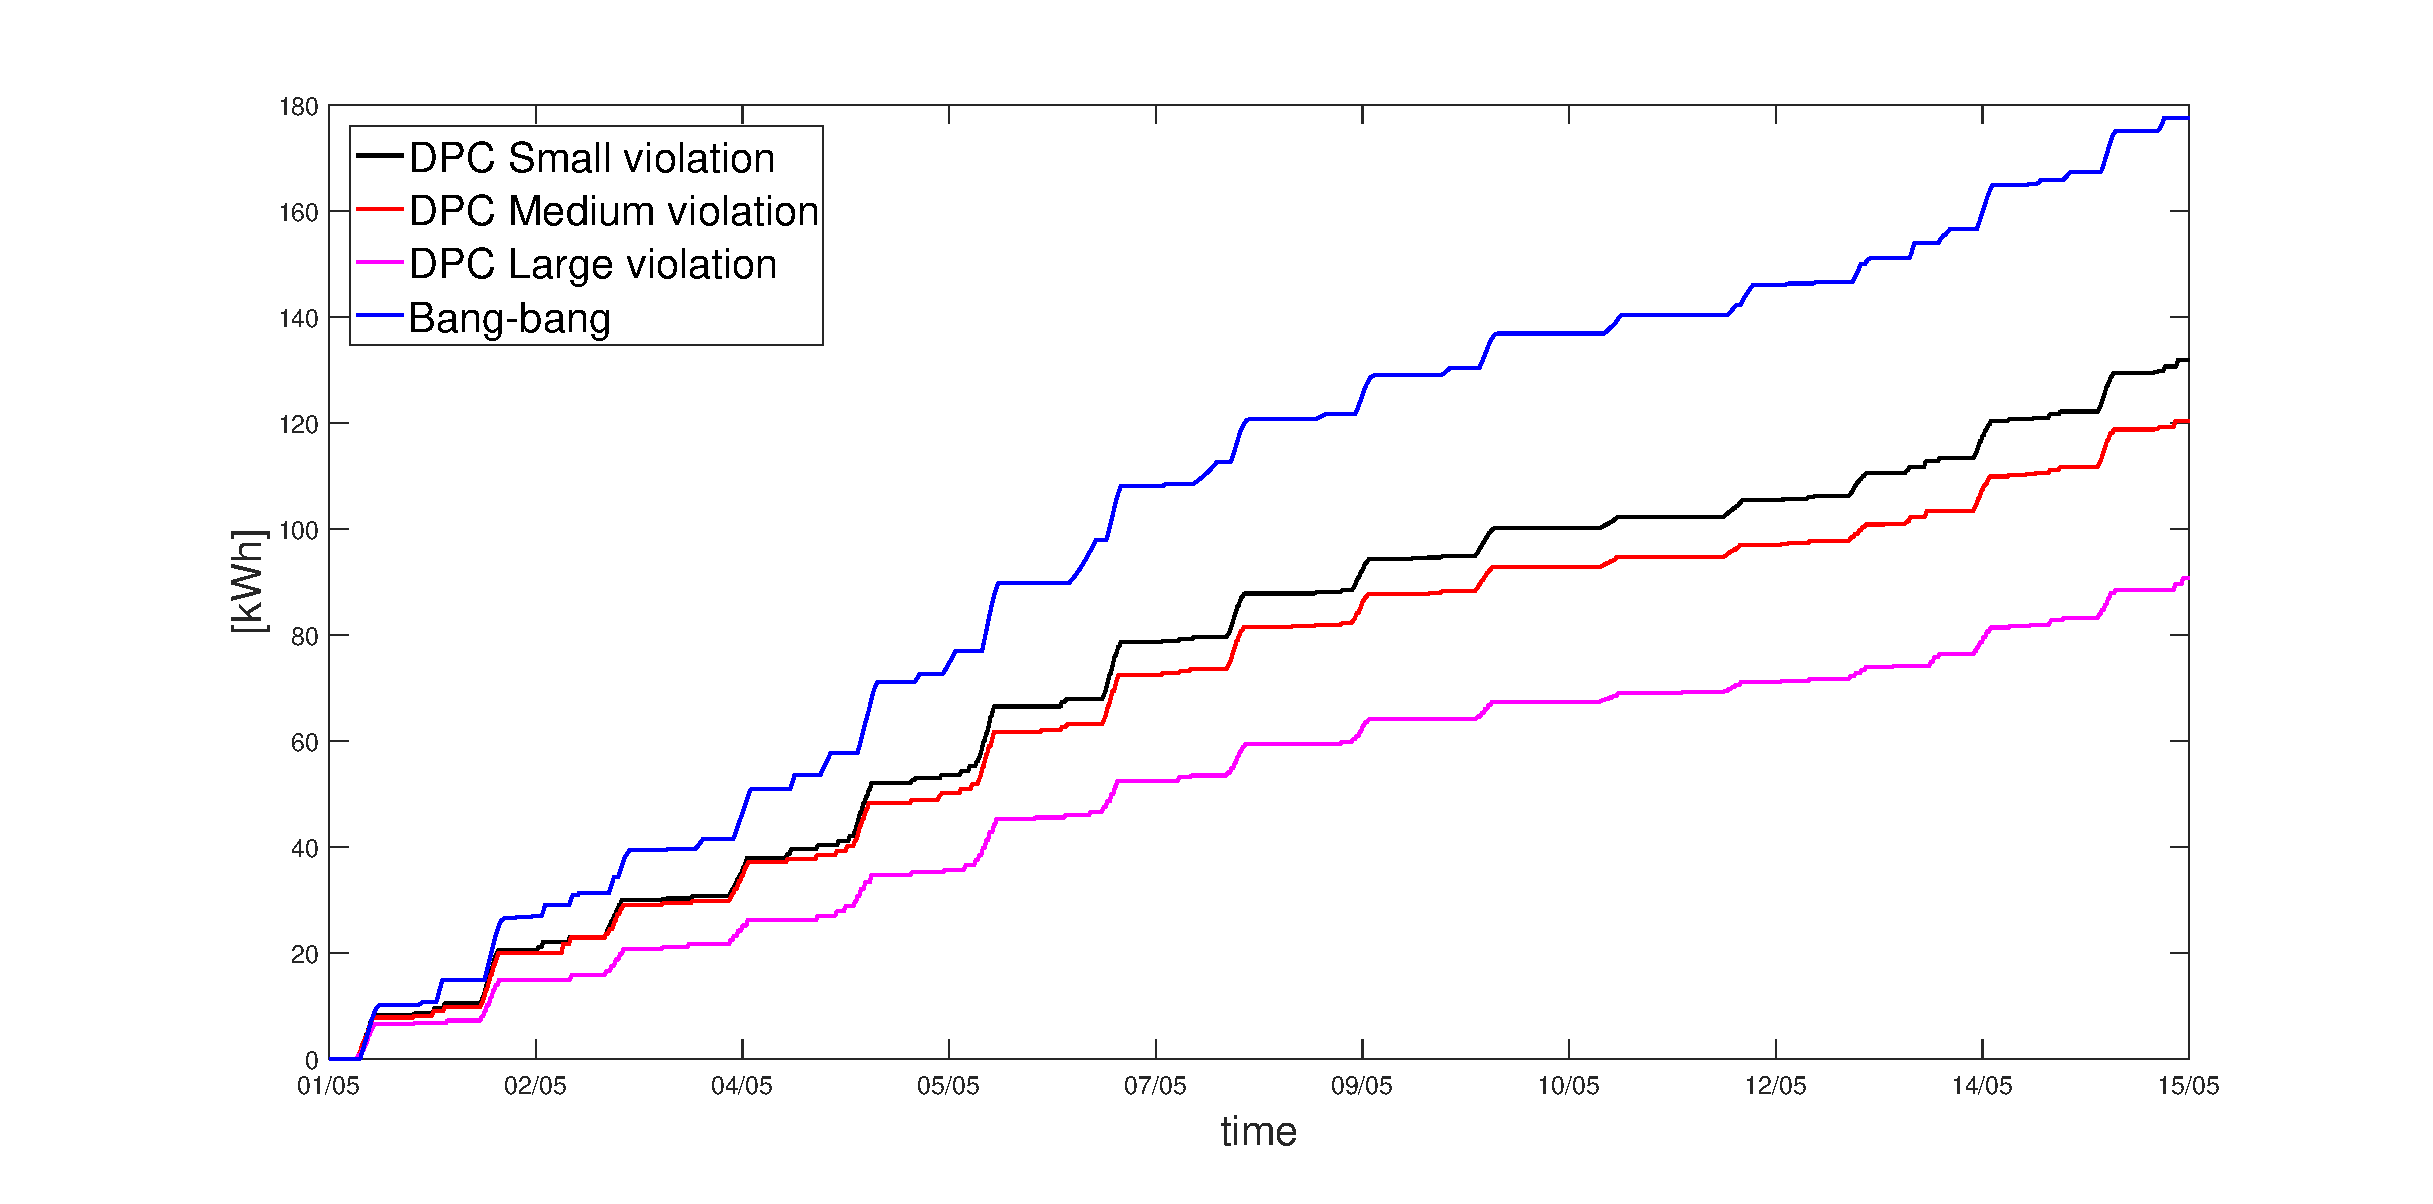
\includegraphics[width=28pc]{figures/Energy_all_EnergyPlus.eps}
	\end{center}
	\caption{Comparison of DPC and bang-bang controller performance over $15$ days of the testing period with different violation configurations, in terms of thermal energy saving using EnergyPlus model. Using bang-bang controller the house energy consumption after $15$ days is of $177kWh$. DPC with small, medium and large violation configurations allows an energy saving of $25.4\%$, $32.3\%$ and $49.2\%$ respectively.}
	\label{F:comparison_all_energy_E+}
\end{figure}

\textcolor[rgb]{0,0,1}{
\subsubsection{Weather forecast subject to uncertainty}\label{SSS:DisturbanceUncertain}
In \cite{Petersen2014AE} the authors investigated, through a large-scale simulation study, the effect of weather forecast uncertainty on the performance of MPC in building systems operations, and compared to the performance of a rule-based strategy.
They considered 48 different scenarios of uncertainties on 72 hours weather forecast.
On such long horizon, results have shown that, with few exceptions, MPC outperforms the rule-based controller in case of energy savings and/or thermal indoor environment, and is in general quite close to the perfect forecast case, despite the uncertainty in weather forecast.}

\textcolor[rgb]{0,0,1}{Horizon length for the DPC algorithm presented in this paper is usually much shorter, as for example $6\ hours$ in Section \ref{S:proof}, $7\ hours$ in Section \ref{S:casestudy}, and $40\ minutes$ in Section \ref{S:realCaseStudy}. This means the weather forecast is more accurate than the 72 hours case presented in \cite{Petersen2014AE}, hence also control performance is even closer to the perfect knowledge forecast case.
Nevertheless, to show the robustness of our approach, in this section we provide simulations considering noisy weather forecast.}

\textcolor[rgb]{0,0,1}{To this aim, we add noises with normal distribution on the disturbance variables in $\X^d$, used to obtain parameters $\hat \Theta$ in the DPC problem \eqref{E:DPCrealcase}, i.e. the disturbance in input in the blue rectangle in Figure \ref{F:overview}, while we use the correct ones to simulate the process, i.e. the disturbance in input in the "Plant" box in the red rectangle in Figure \ref{F:overview}.
In Table \ref{T:NoiseParameters} we summarize the mean and the deviation values of the Gaussian noises that we add to each variable.
We obviously do not add any noise on the "Time of the day" and on the "Day of the week" since those are perfectly known.
We considered zero mean since we suppose there is no constant offset in the forecast, but only an error that can over or underestimate the predictions.
In the table, we also report the range of the values that the variables assumed during the reference period of the historical dataset.
This is to show that the deviation values we chose add a quite bad error on the forecast.
In particular, for example, a deviation of $0.5\degree C$ on the outside air temperature means that the error on the predicted temperature lies within the range of $\pm 1.5\degree C$ with a probability of $99\%$.
We solved DPC problem \ref{P:dpcRealCase} considering the new parameters $\hat \Theta$, obtained using the aforementioned noisy forecast, obtaining the following results, where we show the change in performance on bounds violation and energy consumption due to the forecast inaccuracy.}
\begin{table}[t!]
	\centering	
	\textcolor[rgb]{0,0,1}{\begin{tabular}{lccc}
		\toprule
		Variable               & Range      & Mean & Deviation \\ 
		\midrule
		Outside temperature    & [0,31]     & 0	   & 0.5       \\
		Wind                   & [0,5] 		& 0    & 0.25      \\
		Atmospheric pressure   & [990,1030] & 0    & 50        \\
		Relative Humidity      & [20,91]	& 0    & 5         \\
		Solar Radiation        & [0,1000]   & 0    & 50        \\
		Time of the day        & [0,23]     & 0    & 0         \\
		Day of the week        & [1,7]      & 0    & 0         \\
		\bottomrule
	\end{tabular}}
	\caption{\textcolor[rgb]{0,0,1}{Mean and deviation values of the Gaussian noises added on the weather forecast data, and the range of variation of the variables in the historical dataset.}}
	\captionsetup{justification=centering}
	\label{T:NoiseParameters}
\end{table}

\textcolor[rgb]{0,0,1}{\paragraph{Result 1} In Figure \ref{F:ComparisonTempNoisy} a comparison of the DPC results in terms of temperature control for thermal comfort, between the perfect and the noisy forecast, is shown.
Also here, for the sake of plot's clarity, we show only 4 days and a half of the 15 days simulative period, and we split the plot into 3 sub-figures referring to the small, medium and large violation cases.
We can see that, except for an isolated case in the medium violation case (slightly before the "02/05"), we have a small performance deterioration in terms of bounds violation, although this is more highlighted in the large violation case.
However, the maximum violation, as in the case of perfect forecast, is still lower than $1\,\degree C$.
In particular, we report in Table \ref{T:violationErrorsNoisy} the violation errors in terms of MBE and CV(RMSE) (in $\%$) computed for the whole simulative period, i.e. 15 days.
If we compare them with the ones in Table \ref{T:violationErrors}, we can see that the performance of DPC with noisy forecast are still good with respect to the performance of DPC with perfect forecast, despite the extremely bad prediction error that we considered on the weather forecast.
}
\begin{figure}[t!]
	\begin{center}
		\vspace{1.1cm}
		\subfigure{
			\label{F:SmallNoisy}
			\centering
			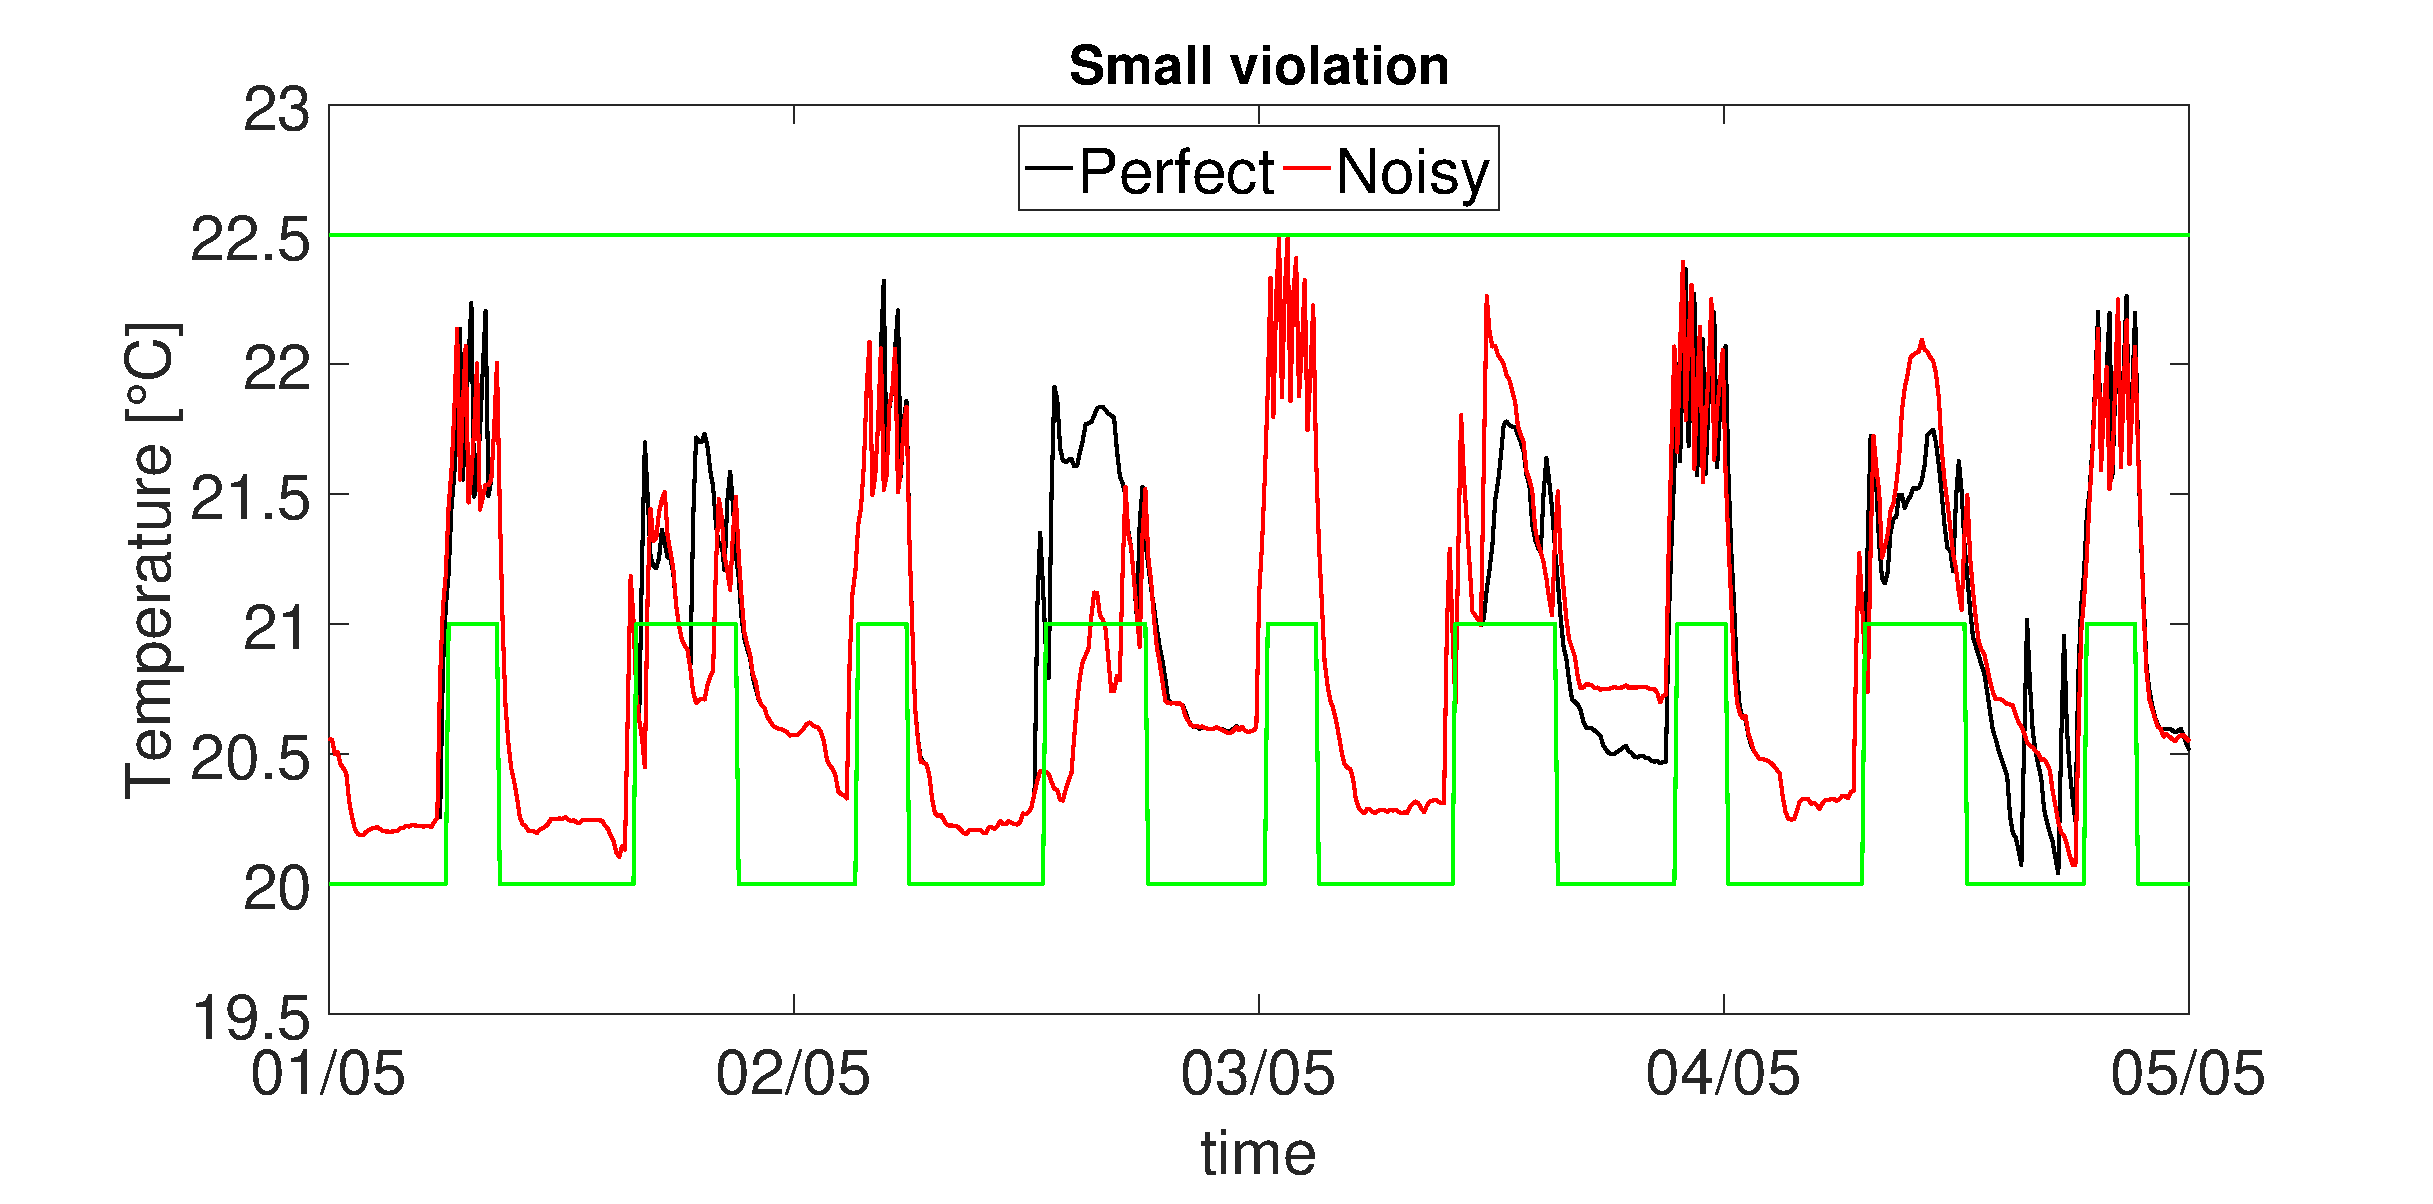
\includegraphics[width=23pc]{figures/Temperatures_small_noisy.eps}
		}	
		\subfigure{
			\label{F:MediumNoisy}
			\centering
			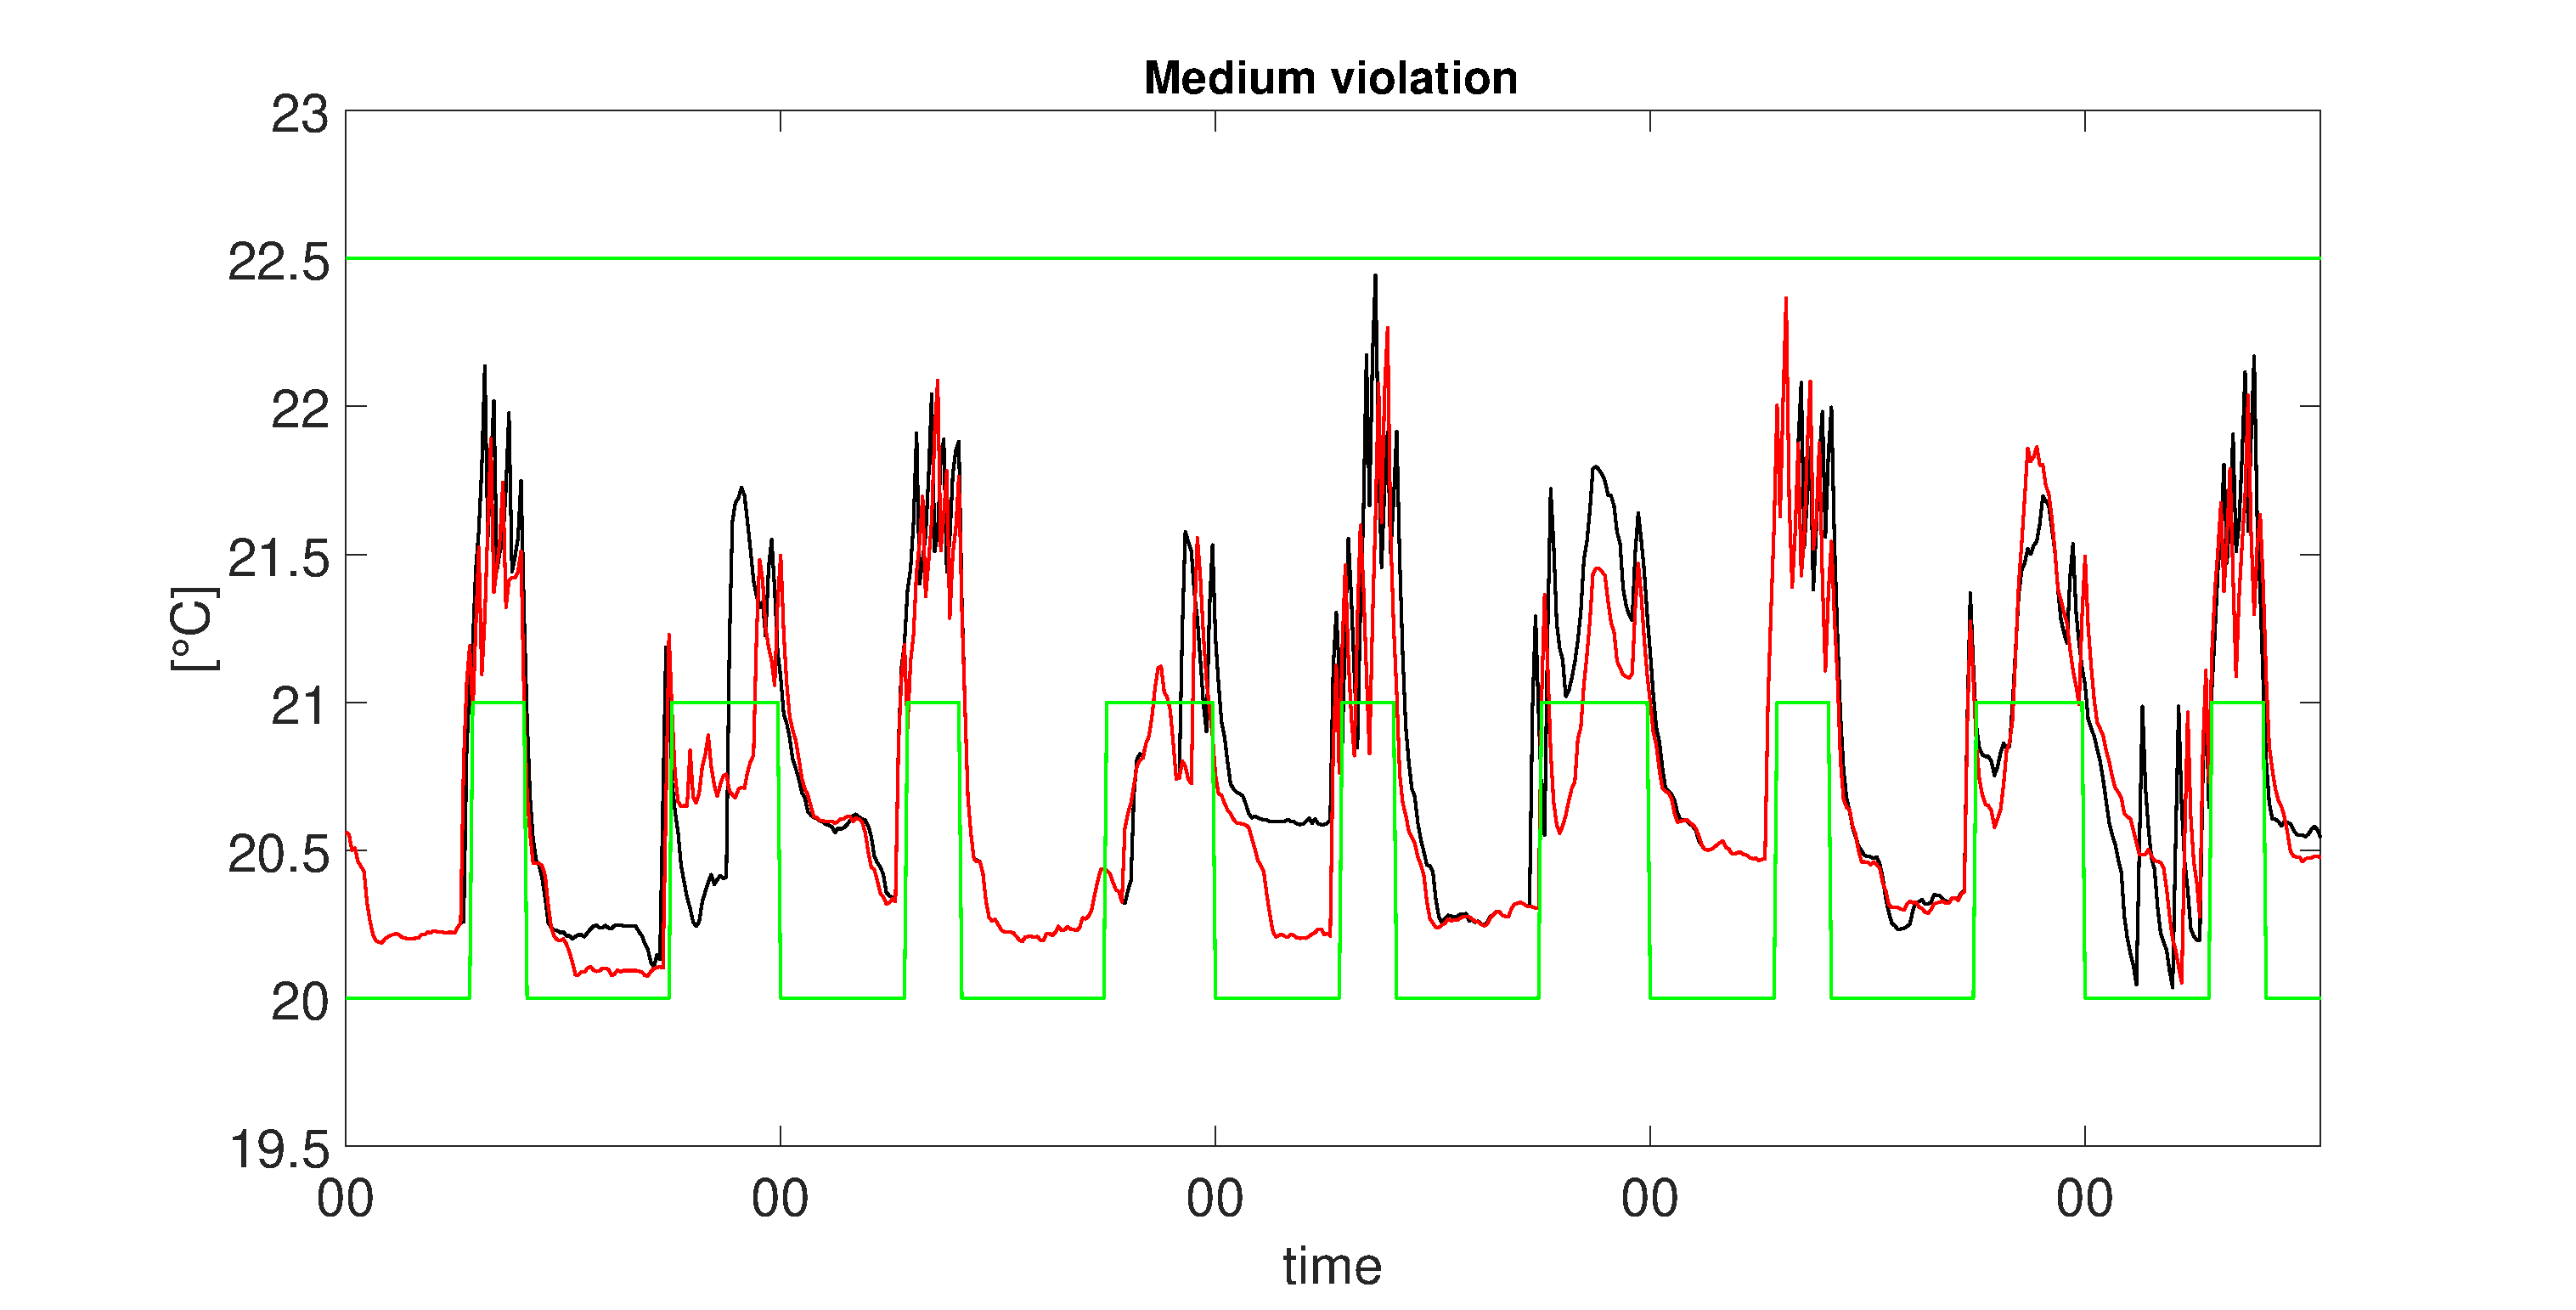
\includegraphics[width=23pc]{figures/Temperatures_medium_noisy.eps}
		}
		\subfigure{
			\label{F:LargeNoisy}
			\centering
			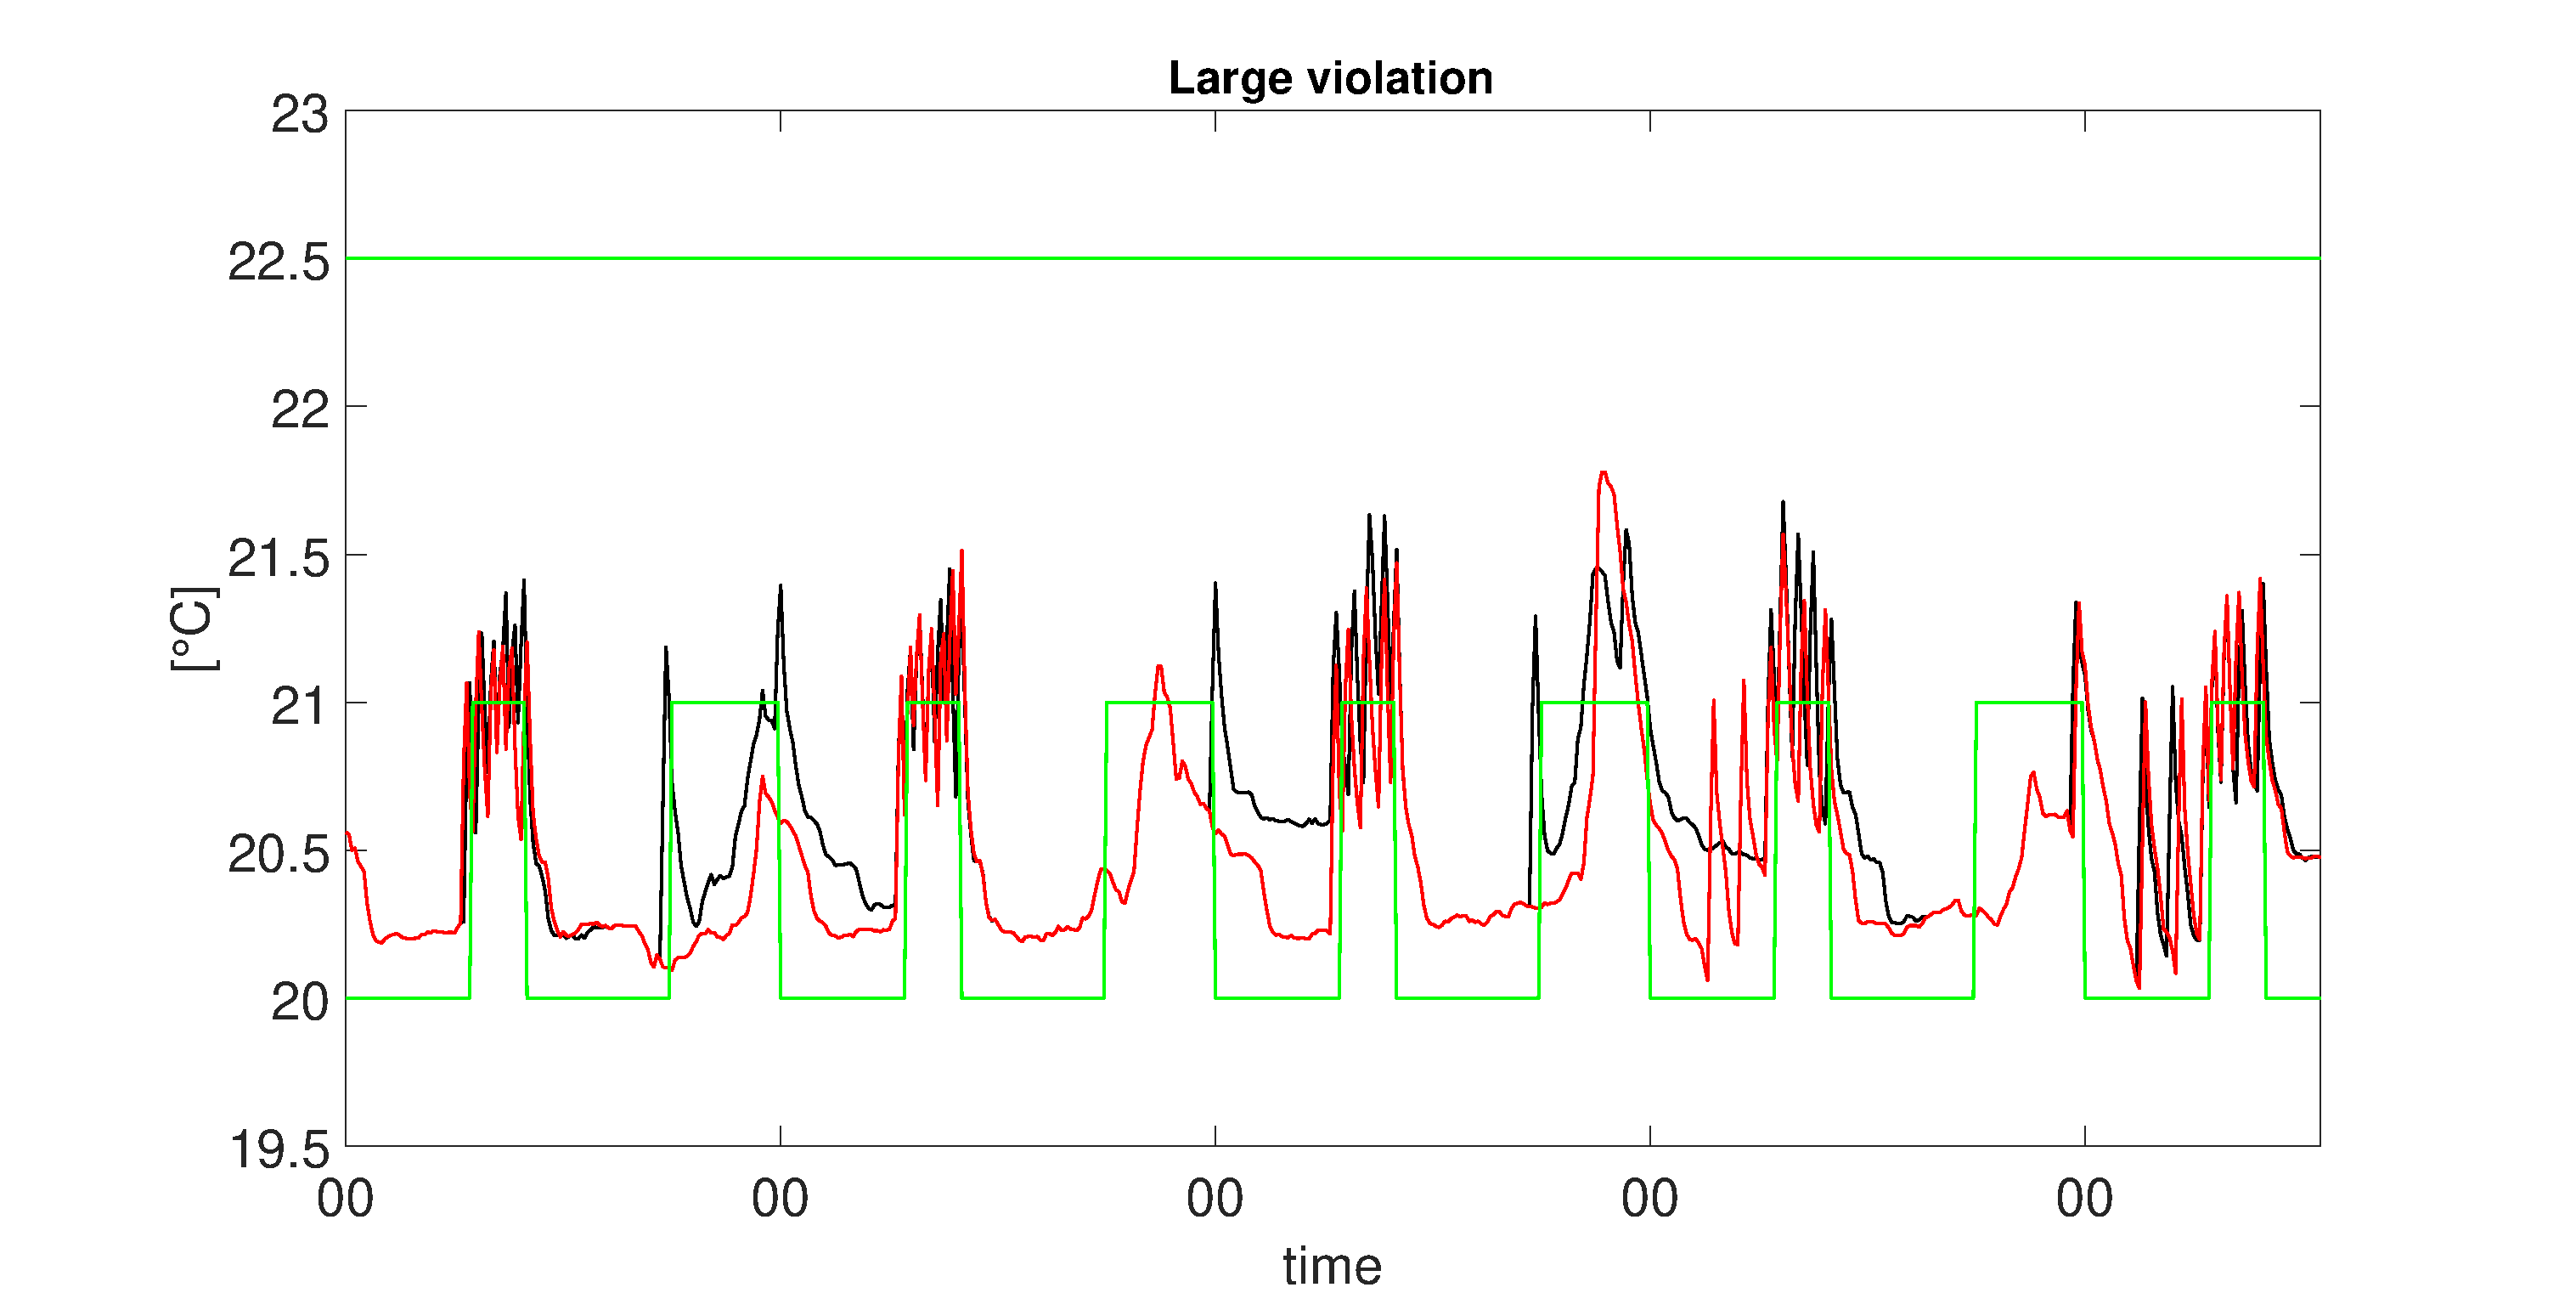
\includegraphics[width=23pc]{figures/Temperatures_large_noisy.eps}
		}	
	\end{center}
	\caption{\textcolor[rgb]{0,0,1}{Comparison of DPC considering perfect and noisy weather forecasts. Small, medium and large violation cases are compared.}}
	\captionsetup{justification=centering}
	\label{F:ComparisonTempNoisy}
\end{figure}

\begin{table}[t!]
	\centering
	%	\scalebox{0.9}{
	\textcolor[rgb]{0,0,1}{\begin{tabular}{lccccc}
		\toprule
		CONTROLLER  & LBV $\mathrm{MBE}$  & LBV $\mathrm{RMSE}$ & UBV $\mathrm{MBE}$ & UBV $\mathrm{RMSE}$ 	\\ 
		\midrule
		$DPC-SV$    & $0.034$             & $0.142$  			      & $0$    				 & $0$     	  	\\
		$DPC-MV$    & $0.178$ 			  & $0.453$       			  & $0$    				 & $0$		  	\\
		$DPC-LV$    & $0.478$  			  & $0.891$     			  & $0$    				 & $0$	      	\\
		\bottomrule
	\end{tabular}}
	%	}
	\caption{\textcolor[rgb]{0,0,1}{Lower Bound Violation (LBV) and Upper Bound Violation (UBV) errors expressed as $\mathrm{MBE}\%$ and $\mathrm{CV(RMSE)}\%$ for DPC Small Violation (DPC-SV), DPC Medium Violation (DPC-MV), DPC large Violation (DPC-LV) and bang-bang controller, considering noisy weather forecast.}}
	\captionsetup{justification=centering}
	\label{T:violationErrorsNoisy}
\end{table}


\textcolor[rgb]{0,0,1}{\paragraph{Result 2} 
In Figure \ref{F:comparison_all_energy_E+_noisy}, we show the difference in terms of energy consumption considering the perfect weather forecast (full line) and the noisy one (dashed line).
We can observe that the case with imperfect forecast is very close to the perfect forecast case.
We recall that we are optimizing a weighted sum of energy and thermal comfort, so depending on the conditions for which the disturbance is over or underestimated, the MPC can require to use more or less energy to supply the prediction errors.
In the small violation case, the energy consumption of the 2 conditions is closer than in the others.
This is because the DPC keeps the temperature within the bounds with an extremely small error in bounds violation.
In particular, the only exception can be seen before May $3^{rd}$ (03/05), where, due to the prediction error, the temperature violates the bounds, so the control uses more energy (than the perfect case) to bring it back above the threshold.
In the other 2 cases, when the temperature violates the bounds, due to the fact that violation constraints are more relaxed, the DPC does not require a too big control effort, hence using less energy.}

\textcolor[rgb]{0,0,1}{These results show the strong robustness of the DPC with respect to errors in the weather forecast.}
\begin{figure}[t!]
	\begin{center}
		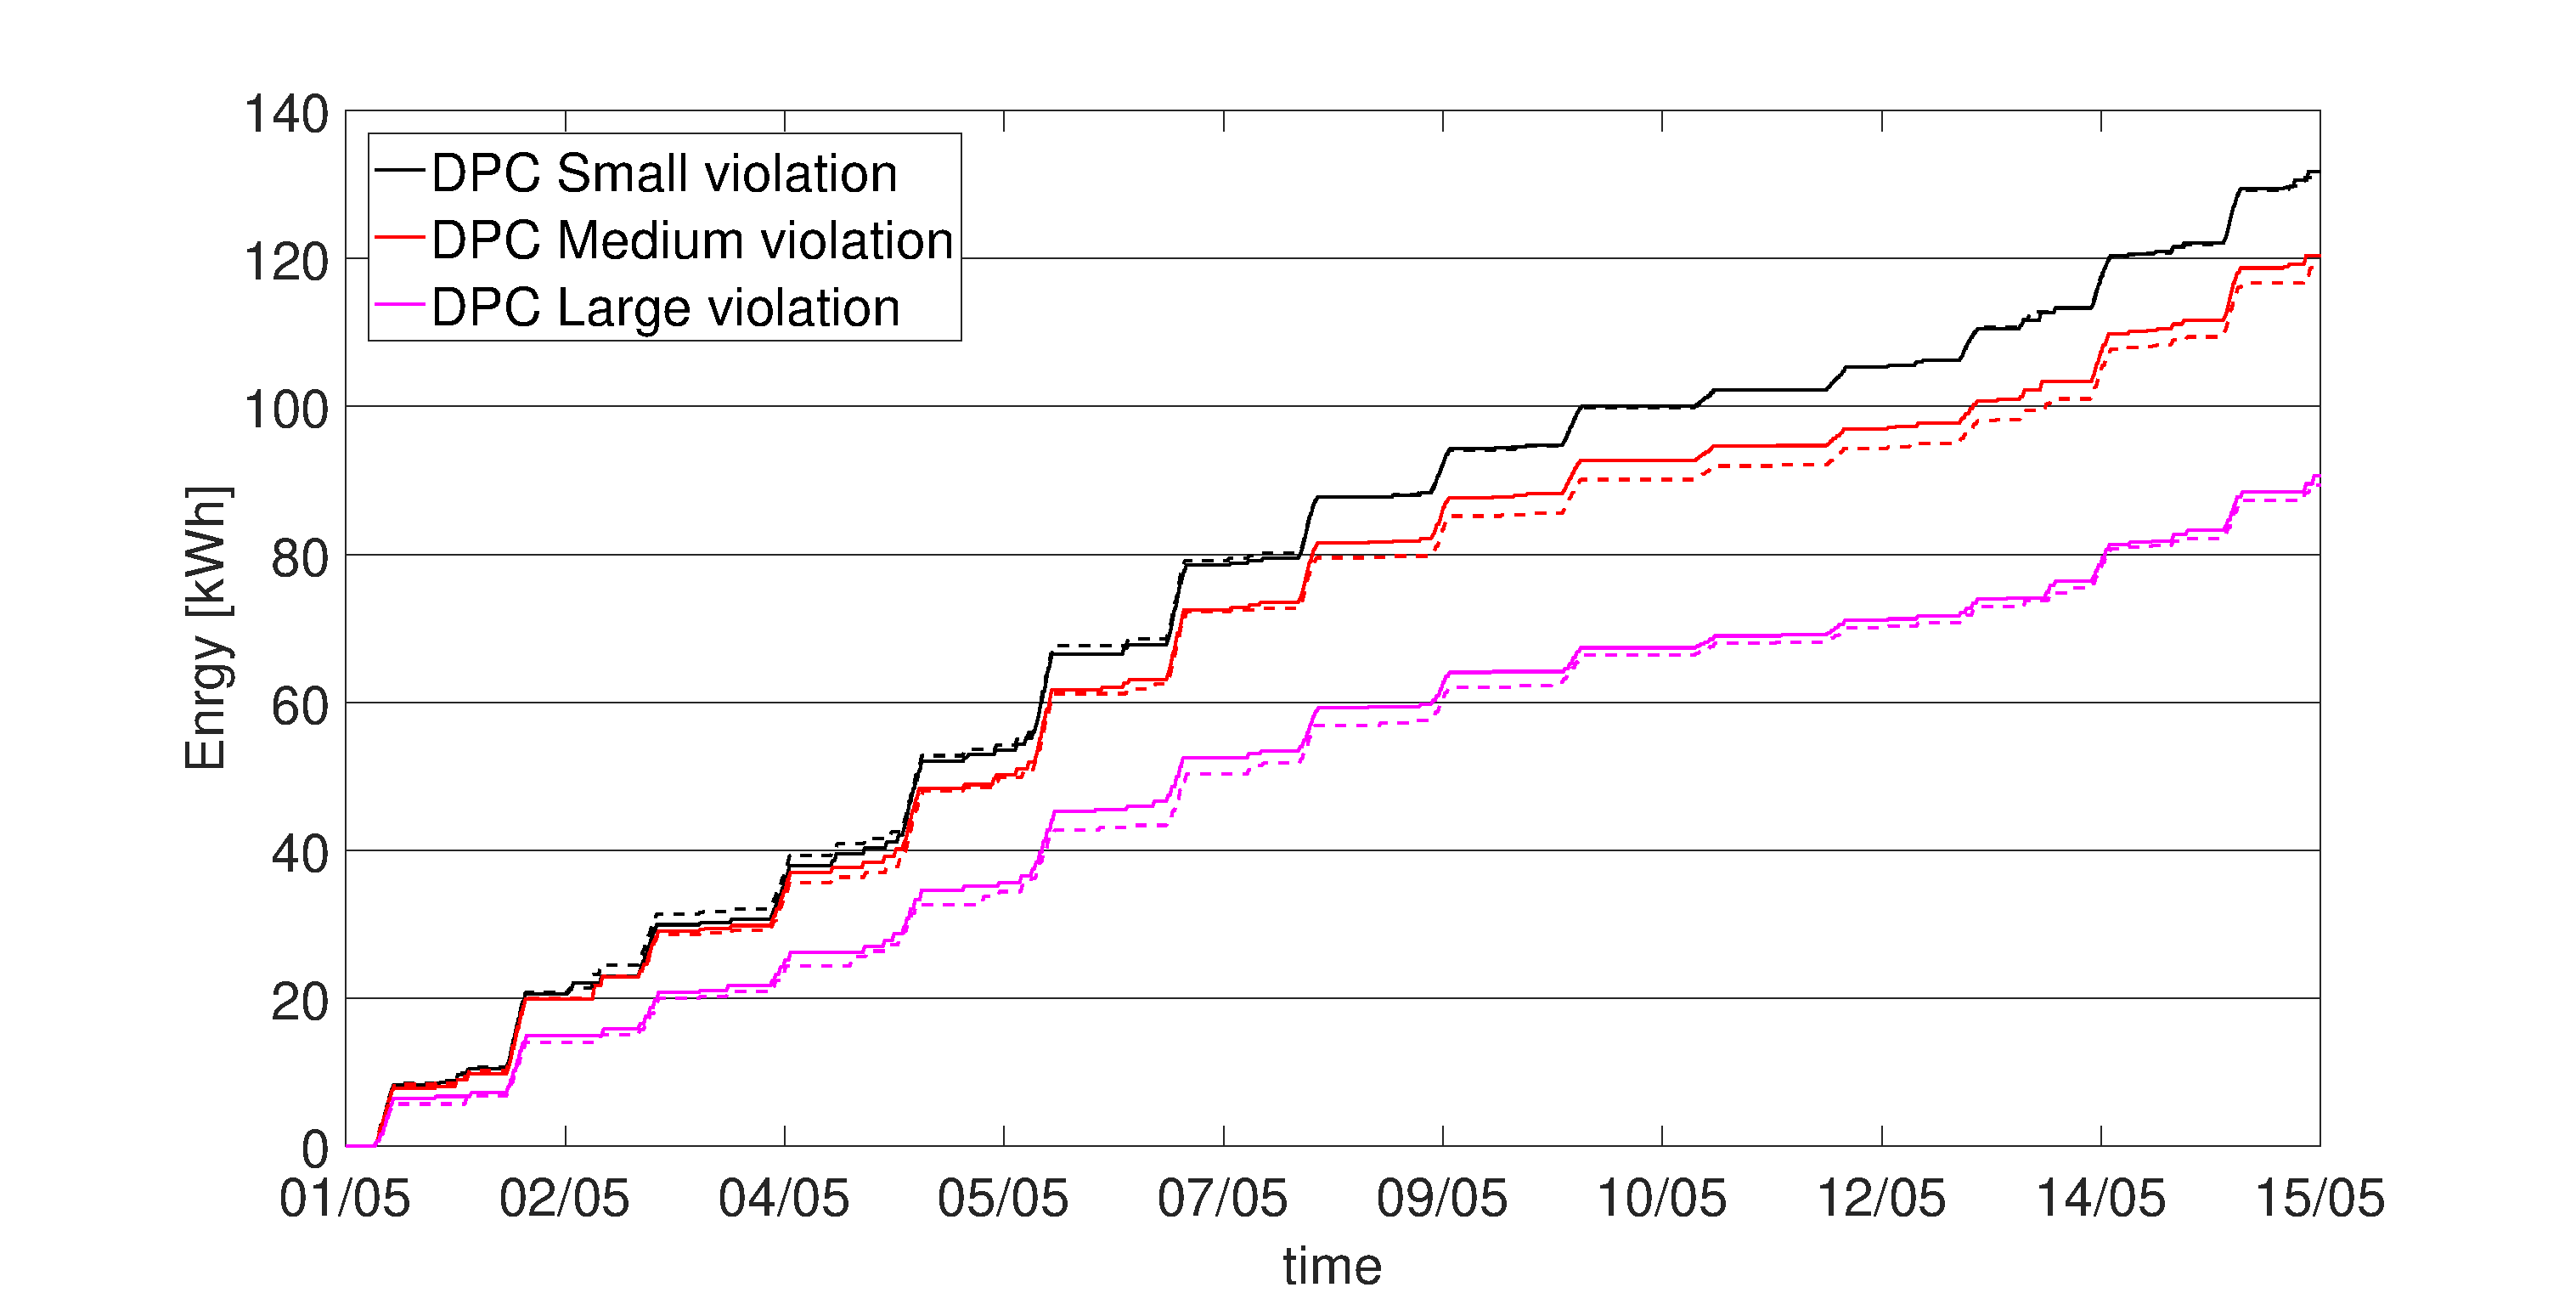
\includegraphics[width=28pc]{figures/Energy_all_EnergyPlus_noisy.eps}
	\end{center}
	\caption{\textcolor[rgb]{0,0,1}{Comparison of DPC in terms of thermal energy saving using EnergyPlus model, considering perfect (full) and imperfect (dashed) weather forecast, over $15$ days of the testing period with different violation configurations. The performance are pretty similar, showing the potential robustness of DPC.}}
	\label{F:comparison_all_energy_E+_noisy}
\end{figure}


%% CONCLUSION
\section{CONCLUSION}
\label{S:conclusion}

To overcome the difficulties associated with the model identification in Model Predictive Control (MPC), we introduce a novel idea for predictive control using data: Data-driven model Predictive Control (DPC). \textcolor[rgb]{0,0,1}{Data-driven control is based on non-physical (black-box) models, therefore they can not be integrated with most of the classical control approaches.} The goal is to create data-driven models that are suitable for receiding horizon control. \textcolor[rgb]{0,0,1}{To this aim, we present two algorithms, based on trees and random forests, to create control-oriented models for DPC. We then apply DPC to three different case studies to demonstrate its strength.}
\begin{enumerate}
\item \emph{\textbf{Comparison with MPC.}} We compare the performance of our DPC to MPC on a multivariable bilinear building model. We establish that DPC with random forests shows a remarkable similarity to MPC in the optimal control strategies explaining $70\%$ variance. On the other hand, DPC with regression trees suffers from practical limitations due to model overfitting.
\item \emph{\textbf{Demand Response application.}} We further apply DPC with random forests to a large scale 6 story EnergyPlus model with 22 zones for which the traditional model-based control is largely unsuitable due to complex dynamics and the cost of model identification. We show that DPC, relying only on the sensor data, can provide significant energy savings while maintaining thermal comfort. Our results demonstrate that even for such complex system, DPC tracks a reference signal with a mean error of $3\%$.
\item \textcolor[rgb]{0,0,1}{\emph{\textbf{Optimal heating system scheduling of a real house.}} We finally apply DPC using experimental data from a real house and compare it with the classical bang-bang controller widely used for temperature control. We show that DPC provides energy savings while guaranteeing thermal comfort for the occupants. With respect to a bang-bang controller, we obtain energy savings that go from $25.4\%$, when we force the temperature to be strictly in a comfort range, to $49.2\%$, if we allow small violations in the thermal comfort level. Furthermore, we demonstrate the robustness of DPC considering uncertainties in the weather forecast.}
\end{enumerate}

DPC has applications which go beyond buildings and energy systems, to industrial process control, and controlling large critical infrastructures like water networks, district heating \& cooling. DPC is immensely valuable in situations where first principles based modeling cost is extremely high.

\subsection{Practical Challenges and Future Work}
\label{SS:challenges}
\begin{enumerate}
\item \emph{\textbf{Data Availability:}} The main practical challenge for DPC lies in the availability of data for training, and we require answers to questions like \emph{how much data (functional testing) is required, and how should the sampling be done?} Therefore, the procedure for optimal experiment design, and model improvement with estimation of variance in predictions is one of the main focus of our ongoing work.
\item \emph{\textbf{Stability:}} While the buildings are inherently stable, many other applications require stability guarantees. In our ongoing work, we are working towards proving asymptotic stability to origin with DPC-RT and DPC-En by using concept of switched LTI systems. This will make DPC useful for systems with faster dynamics.
\end{enumerate}

%ACKNOWLEDGMENTS
\section*{ACKNOWLEDGMENT}
This work was supported partially by the Italian Government under Cipe resolution n.135 (Dec. 21, 2012), project \emph{INnovating City Planning through Information and Communication Technologies} (INCIPICT), and by TerraSwarm, one of six centers of STARnet, a Semiconductor Research Corporation program sponsored by MARCO and DARPA.

The authors would like to thank Xiaojing Zhang, a PostDoctoral Researcher at the University of California, Berkeley, for providing the bilinear building model, Iole Nardi, a PostDoctoral Researcher at the University of L'Aquila, for the help in obtaining the real data from the house, and Manfred Morari, for his feedback on DPC.

\newpage
%% BIBLIOGRAPHY
\section*{References}
\bibliographystyle{elsarticle-num}
\bibliography{fsRefs,achinRefs}

\end{document}